% This is FinalProjectReport.tex, using the LLNCS macro package for
% Springer Computer Science proceedings.
% Version 2.21 of 2022/01/12
%
\documentclass[runningheads]{llncs}
%
\usepackage[T1]{fontenc}
% T1 fonts will be used to generate the final print and online PDFs,
% so please use T1 fonts in your manuscript whenever possible.
% Other font encondings may result in incorrect characters.
%
\usepackage{graphicx}
% Used for displaying a sample figure. If possible, figure files should
% be included in EPS format.
%
\usepackage{booktabs}
\usepackage{amsmath}
\usepackage{subcaption}
\usepackage{placeins} % provides \FloatBarrier (used manually in the appendix)
\usepackage{float}     % provides the [H] specifier to pin a figure exactly in place
\usepackage{eso-pic}   % absolute placement of the cover-page logos
%
% If you use the hyperref package, please uncomment the following two lines
% to display URLs in blue roman font according to Springer's eBook style:
\usepackage{color}
\usepackage{hyperref}
\renewcommand\UrlFont{\color{blue}\rmfamily}
\urlstyle{rm}
%
\graphicspath{{../../results/figures/}{../../results/gradcam/}{./}}
%
% Allow a little extra inter-word stretch to avoid overfull lines caused by
% long hyphenated compounds and \texttt{} tokens, and give hyphenation hints.
\emergencystretch=3em
\raggedbottom
% Relax the float-placement parameters so figures/tables sit closer to the
% text that references them (more float area per page, less forced text).
\renewcommand{\topfraction}{0.92}
\renewcommand{\bottomfraction}{0.85}
\renewcommand{\textfraction}{0.08}
\renewcommand{\floatpagefraction}{0.75}
\setcounter{topnumber}{3}
\setcounter{bottomnumber}{2}
\setcounter{totalnumber}{5}
% Silence purely cosmetic "underfull hbox" reports (loose inter-word spacing
% that is invisible in the PDF); genuine overfull boxes are still reported.
\hbadness=10000
\hfuzz=0.5pt
\hyphenation{probabil-ity-averaging depend-ency-pinned trans-fer-learning
re-sam-pling aeti-ology DenseNet ResNet ImageNet}
%
\begin{document}
%
\title{Deep Learning for Pneumonia Classification from
Pediatric Chest X-Rays: From a Binary Baseline to a
Bacterial--Viral Three-Class Extension}
%
\titlerunning{Deep Learning for Pediatric Pneumonia Classification}
%
\author{Carolina Reis\inst{1} \and
Jakub B\l{}aszczyk\inst{1,2}}
%
\authorrunning{C. Reis and J. B\l{}aszczyk}
%
\institute{University of Aveiro, Aveiro, Portugal\\
\email{\{luanacarolina,jakub.blaszczyk\}@ua.pt} \and
Lodz University of Technology, \L{}\'od\'z, Poland}
%
\maketitle              % typeset the header of the contribution
%
% Cover-page logos: UA top-left, DETI top-right (first page only).
\AddToShipoutPictureBG*{%
  \AtPageUpperLeft{\raisebox{-1.6cm}{\hspace{1.6cm}%
    
\includegraphics[height=0.9cm]{logo-ua.png}}}%
  \AtPageUpperLeft{\hspace{\paperwidth}\raisebox{-1.6cm}{%
    \makebox[0pt][r]{
\includegraphics[height=0.9cm]{logo-deti.png}\hspace{1.6cm}}}}%
}
%
\begin{abstract}
Pneumonia is a leading cause of pediatric mortality worldwide, and chest
X-ray (CXR) interpretation remains a bottleneck in resource-limited
settings. We study deep-learning models for pneumonia classification on
the public Kermany pediatric CXR dataset. As a baseline we address the
standard binary task (NORMAL vs.\ PNEUMONIA), comparing a custom
convolutional neural network (CNN) against ImageNet-pretrained ResNet18
and DenseNet121 transfer-learning models. Following feedback to increase
the clinical relevance of the task, we extend the problem to a
three-class formulation that separates \emph{bacterial} from
\emph{viral} pneumonia---a distinction that drives different treatment
decisions---using labels derived automatically from the dataset
filenames. We further investigate a probability-averaging ensemble, model
calibration (Expected Calibration Error and reliability diagrams),
decision-threshold optimisation for two clinical scenarios, and Grad-CAM
visual explanations that verify the models attend to clinically plausible
lung regions. On the binary task the ensemble reaches an accuracy of
$0.856$, an F1 of $0.896$, and an AUROC of $0.963$ with $99.7\%$ recall
on pneumonia (only $1$ of $390$ cases missed). On the harder three-class
task, evaluated with a leakage-free patient-aware split, the ensemble
achieves an accuracy of $0.822$ and a macro-F1 of $0.808$, with per-class
F1 scores of $0.78$ (NORMAL), $0.92$ (BACTERIA), and $0.72$ (VIRUS),
confirming that viral pneumonia is the most difficult class to recognise. All experiments are reproducible across three seeds and
are released as an open, documented code repository.

\keywords{Pneumonia classification \and Chest X-ray \and Transfer
learning \and Convolutional neural networks \and Grad-CAM \and Model
calibration.}
\end{abstract}
%
%
%
\section{Introduction}

Pneumonia is an acute respiratory infection of the lungs and one of the
leading causes of death in children under five years of age worldwide.
Chest X-ray (CXR) imaging is the most widely used and accessible modality
for diagnosing pneumonia, but its interpretation requires trained
radiologists, who are scarce in many low-resource settings. Computer-aided
diagnosis systems based on deep learning have therefore attracted strong
interest as a way to support, triage, and accelerate radiological
workflows.

In this work we develop and evaluate deep-learning models for pneumonia
classification from pediatric CXR images, using the public
Kermany ``Chest X-Ray Images (Pneumonia)'' dataset~\cite{ref_kermany}.
The project is organised around two tasks. The first is the standard
\emph{binary} task of distinguishing NORMAL from PNEUMONIA, which we use
as a baseline to compare a custom CNN against two transfer-learning
backbones. The second, and our main contribution, is a \emph{three-class}
extension that further separates pneumonia into its \emph{bacterial} and
\emph{viral} subtypes. This distinction is clinically meaningful: bacterial
pneumonia is typically treated with antibiotics, whereas viral pneumonia is
not, so a model that can hint at the likely aetiology is potentially more
useful in practice than one that only flags the presence of disease.

Our contributions are the following:
\begin{enumerate}
  \item A clean, reproducible comparison of a custom CNN, ResNet18, and
  DenseNet121 on binary pediatric pneumonia classification, reported as
  mean\,$\pm$\,standard deviation across three random seeds.
  \item A three-class (NORMAL / BACTERIA / VIRUS) extension whose labels are
  derived automatically from the dataset filenames, requiring no manual
  annotation, together with a per-class analysis of where the models
  succeed and fail.
  \item A study of additional, clinically motivated components: a
  probability-averaging ensemble, a calibration analysis (Expected
  Calibration Error and reliability diagrams), decision-threshold
  optimisation for two clinical scenarios, and Grad-CAM visual
  explanations.
  \item A documented, dependency-pinned code repository with
  command-line entry points that reproduce every result and figure in
  this report.
\end{enumerate}

This repository is intended for educational experimentation only and is
not a clinical decision tool.

\section{Related Work}

The release of large public CXR datasets greatly accelerated research on
pneumonia detection. Wang et al.~\cite{ref_chestxray14} introduced
ChestX-ray14, and Rajpurkar et al.~\cite{ref_chexnet} proposed CheXNet, a
121-layer DenseNet that matched radiologist performance on pneumonia
detection, establishing DenseNet as a strong backbone for CXR analysis.
Kermany et al.~\cite{ref_kermany} released the pediatric CXR dataset used
in this work and demonstrated the effectiveness of transfer learning from
ImageNet-pretrained networks for medical image classification, a strategy
that remains a standard and competitive baseline.

Transfer learning is particularly attractive in the medical domain because
labelled data is limited: deep features learned on ImageNet~\cite{ref_imagenet,ref_alexnet}
transfer well to CXRs, and only the classifier head (and optionally the
deeper layers) needs to be retrained~\cite{ref_kermany,ref_chexnet}. This
approach has been applied repeatedly to pneumonia detection on the Kermany
dataset with strong results~\cite{ref_rahman}. To make such models
trustworthy, two complementary tools are widely used. Grad-CAM~\cite{ref_gradcam}
produces class-discriminative heatmaps that reveal which image regions a CNN
relies on, helping to detect spurious correlations. Calibration analysis,
summarised by the Expected Calibration Error and reliability
diagrams~\cite{ref_calibration,ref_naeini}, quantifies whether predicted
probabilities reflect true correctness likelihood---an important property
when a model's output is used to set a decision threshold in a screening or
assisted-diagnosis pipeline. Finally, ensembling independently trained
models is a simple and reliable way to reduce variance and improve
robustness~\cite{ref_ensemble}, and ensembles of CNNs have been shown to
boost pneumonia-detection performance specifically~\cite{ref_kundu}.

Most prior work on the Kermany dataset addresses only the binary task. The
bacterial-versus-viral distinction is encoded in the filenames but is
rarely exploited. Our three-class extension targets exactly this gap and
analyses it under the same reproducible protocol as the binary baseline.

\section{Dataset}

We use the Kermany pediatric ``Chest X-Ray Images
(Pneumonia)'' dataset~\cite{ref_kermany,ref_kaggle}, which contains
anterior--posterior CXRs of pediatric patients (ages 1--5) collected at the
Guangzhou Women and Children's Medical Center. The dataset ships with a
fixed train/validation/test split and two top-level classes, NORMAL and
PNEUMONIA. We use the provided split as-is.

For the three-class task we exploit the fact that every pneumonia image
encodes its aetiology in the filename
(e.g.\ \texttt{person100\_bacteria\_4.jpeg} vs.\
\texttt{person154\_virus\_2.jpeg}). A small parser maps each file to one of
NORMAL, BACTERIA, or VIRUS, so the three-class labels are obtained
automatically and require no manual annotation. Table~\ref{tab:dataset}
summarises the resulting class counts and Fig.~\ref{fig:dist} visualises
the binary split.

\begin{table}[!ht]
\caption{Image counts for the binary and three-class formulations. The
provided validation split contains only 16 images, so for the three-class
task a small balanced validation set (8 images per class) is re-sampled
deterministically from the training data when classes are missing.}
\label{tab:dataset}
\centering
\begin{tabular}{lrrrr}
\toprule
Split & NORMAL & BACTERIA & VIRUS & Total \\
\midrule
Train & 1{,}341 & 2{,}530 & 1{,}345 & 5{,}216 \\
Test  & 234     & 242     & 148     & 624 \\
\bottomrule
\end{tabular}
\end{table}

Two characteristics of the dataset shape our methodology. First, the
training set is \emph{class-imbalanced}: PNEUMONIA images outnumber NORMAL
images roughly $2.9\!:\!1$, and within pneumonia, bacterial cases dominate
viral cases. Second, the official validation split is tiny (16 images),
which makes model selection noisy; for the three-class task we therefore
re-sample a small balanced validation set from the training data with a
fixed seed whenever a class is missing. All reported metrics are computed
on the untouched official test set of 624 images.

\begin{figure}[H]
\centering
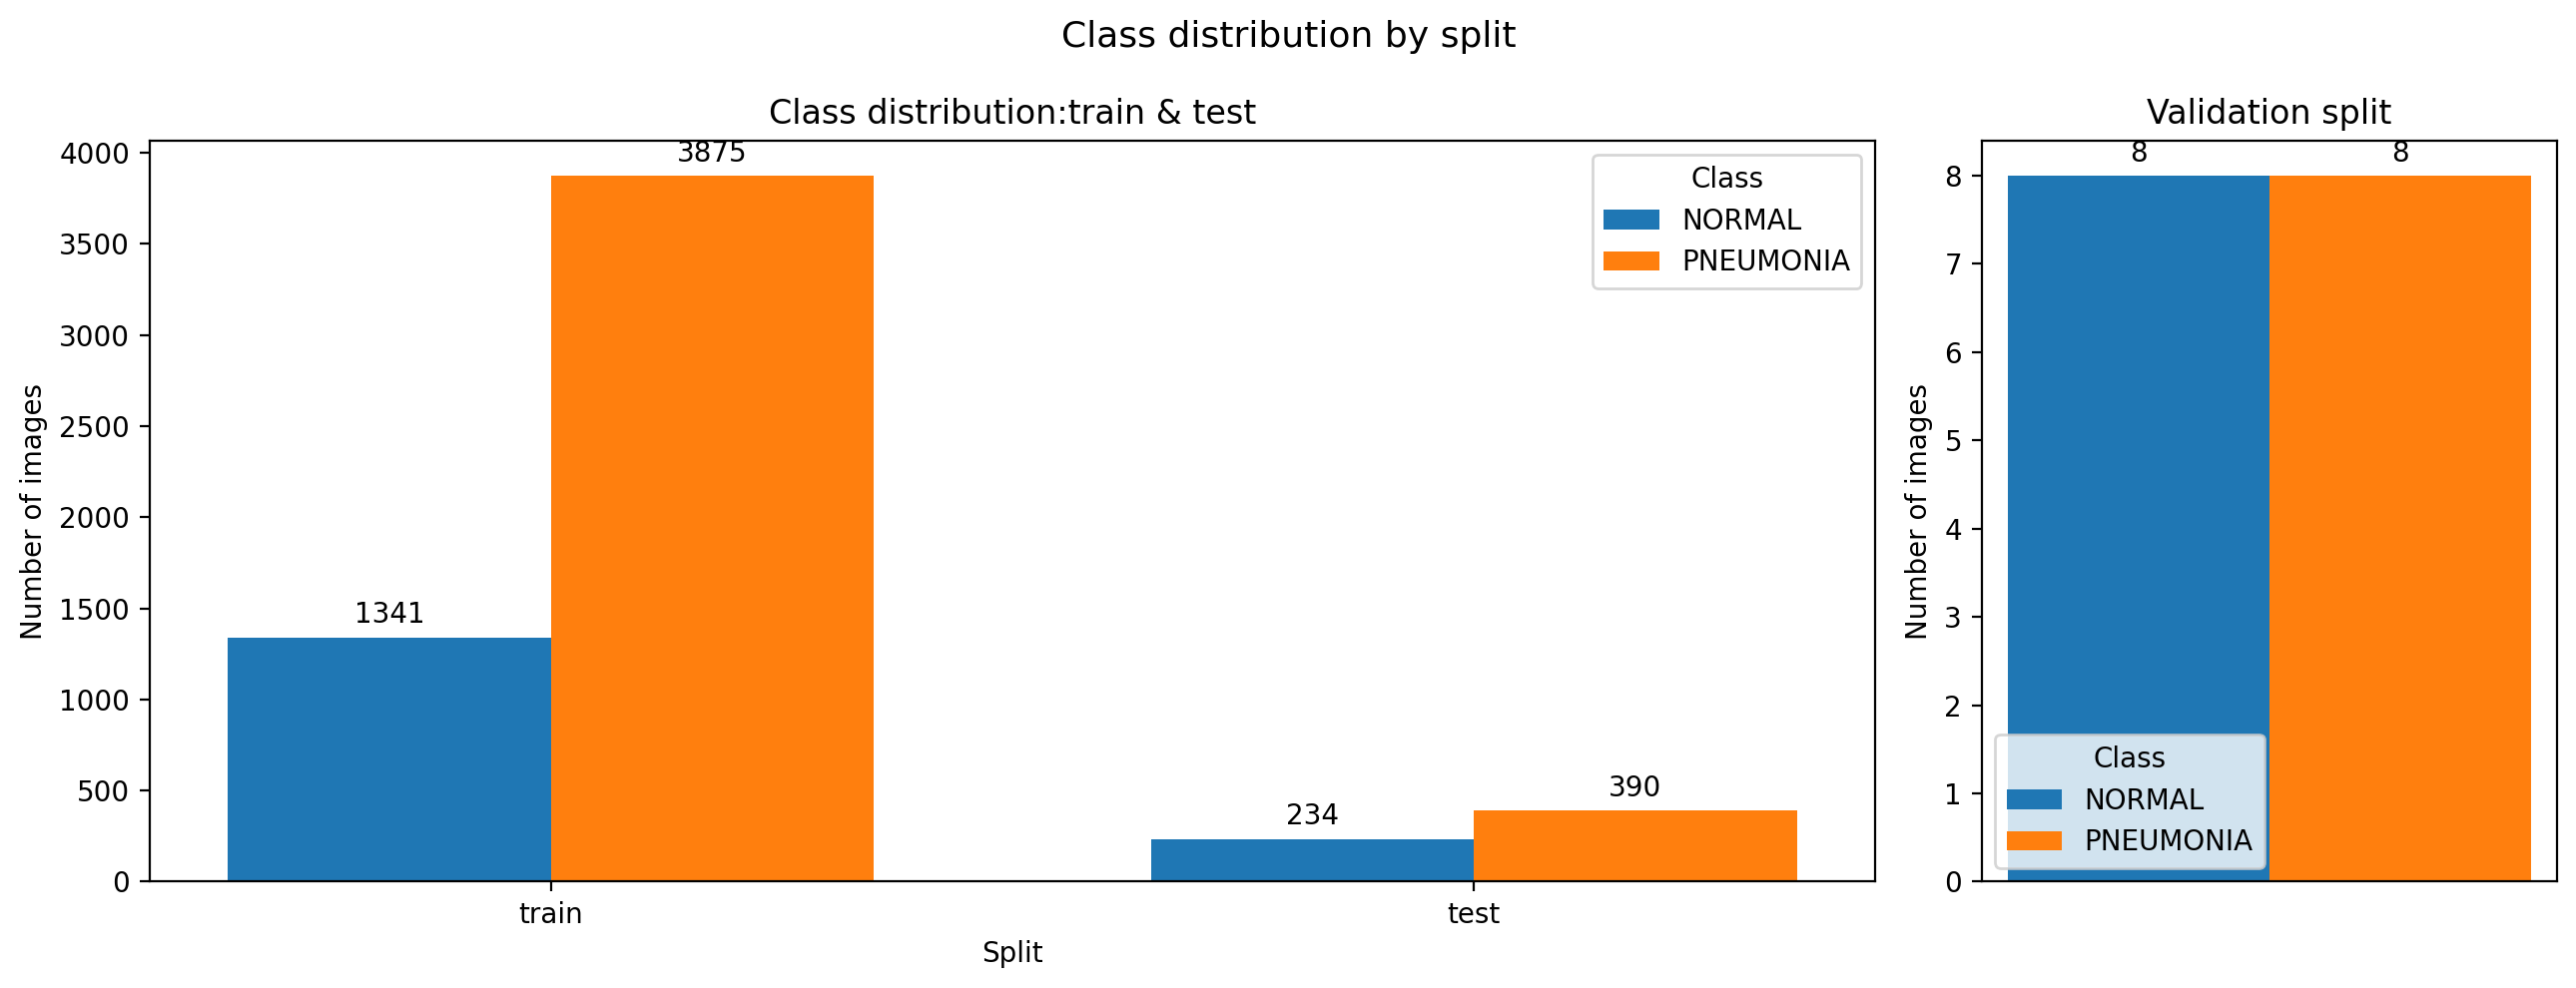
\includegraphics[width=\textwidth]{class_distribution.png}
\caption{Binary class distribution by split. \emph{Left:} the training and
test sets are dominated by PNEUMONIA ($\approx2.9\!:\!1$ in training).
\emph{Right:} the official validation split contains only 16 images,
motivating the re-sampling strategy used for the three-class task.}
\label{fig:dist}
\end{figure}

\section{Methodology}

\subsection{Preprocessing and Augmentation}

All images are resized to $224\times224$ pixels. Because the pretrained
backbones expect three-channel RGB input, the grayscale X-rays are
converted to three channels, and ImageNet normalisation
(mean $[0.485, 0.456, 0.406]$, std $[0.229, 0.224, 0.225]$) is applied.
During training we use light data augmentation appropriate for
radiographs---random horizontal flips and small rotations
($\pm10^{\circ}$)---which preserves diagnostic content while improving
generalisation. Validation and test images are not augmented.

\subsection{Models}

We compare three architectures.

\textbf{Custom CNN (baseline).} A compact three-block convolutional network.
Each block is a $3\times3$ convolution followed by batch normalisation, a
ReLU activation, and $2\times2$ max-pooling, with the channel width growing
$32\!\to\!64\!\to\!128$. A global average-pooling layer, dropout
($p=0.3$), and a single linear layer produce the output. This model is
trained from scratch and serves as a lower-bound reference.

\textbf{ResNet18}~\cite{ref_resnet} and \textbf{DenseNet121}~\cite{ref_densenet}.
Two standard ImageNet-pretrained backbones (see also the accessible
overviews in~\cite{ref_vizuara_resnet,ref_vizuara_densenet}). We replace the
final classification layer with a new linear head sized for the task (one
output for binary, three for the three-class task) and apply transfer learning.

The two backbones differ in how they reuse features
(Fig.~\ref{fig:architectures}). ResNet uses \emph{residual} (skip)
connections that add a block's input to its output ($x + F(x)$), easing
gradient flow in deep networks; DenseNet instead \emph{concatenates} each
layer's output with all preceding feature maps, maximising feature reuse with
fewer parameters.

\begin{figure}[H]
\centering
\begin{subfigure}{0.49\textwidth}
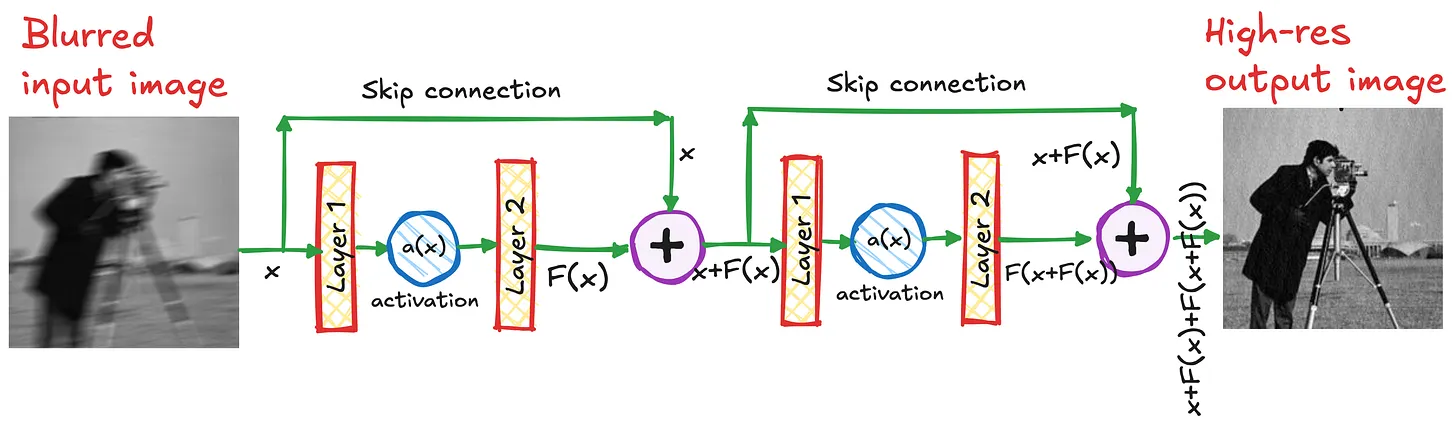
\includegraphics[width=\textwidth]{resnet-explanation.png}
\caption{ResNet: residual (skip) connections.}
\end{subfigure}\hfill
\begin{subfigure}{0.49\textwidth}
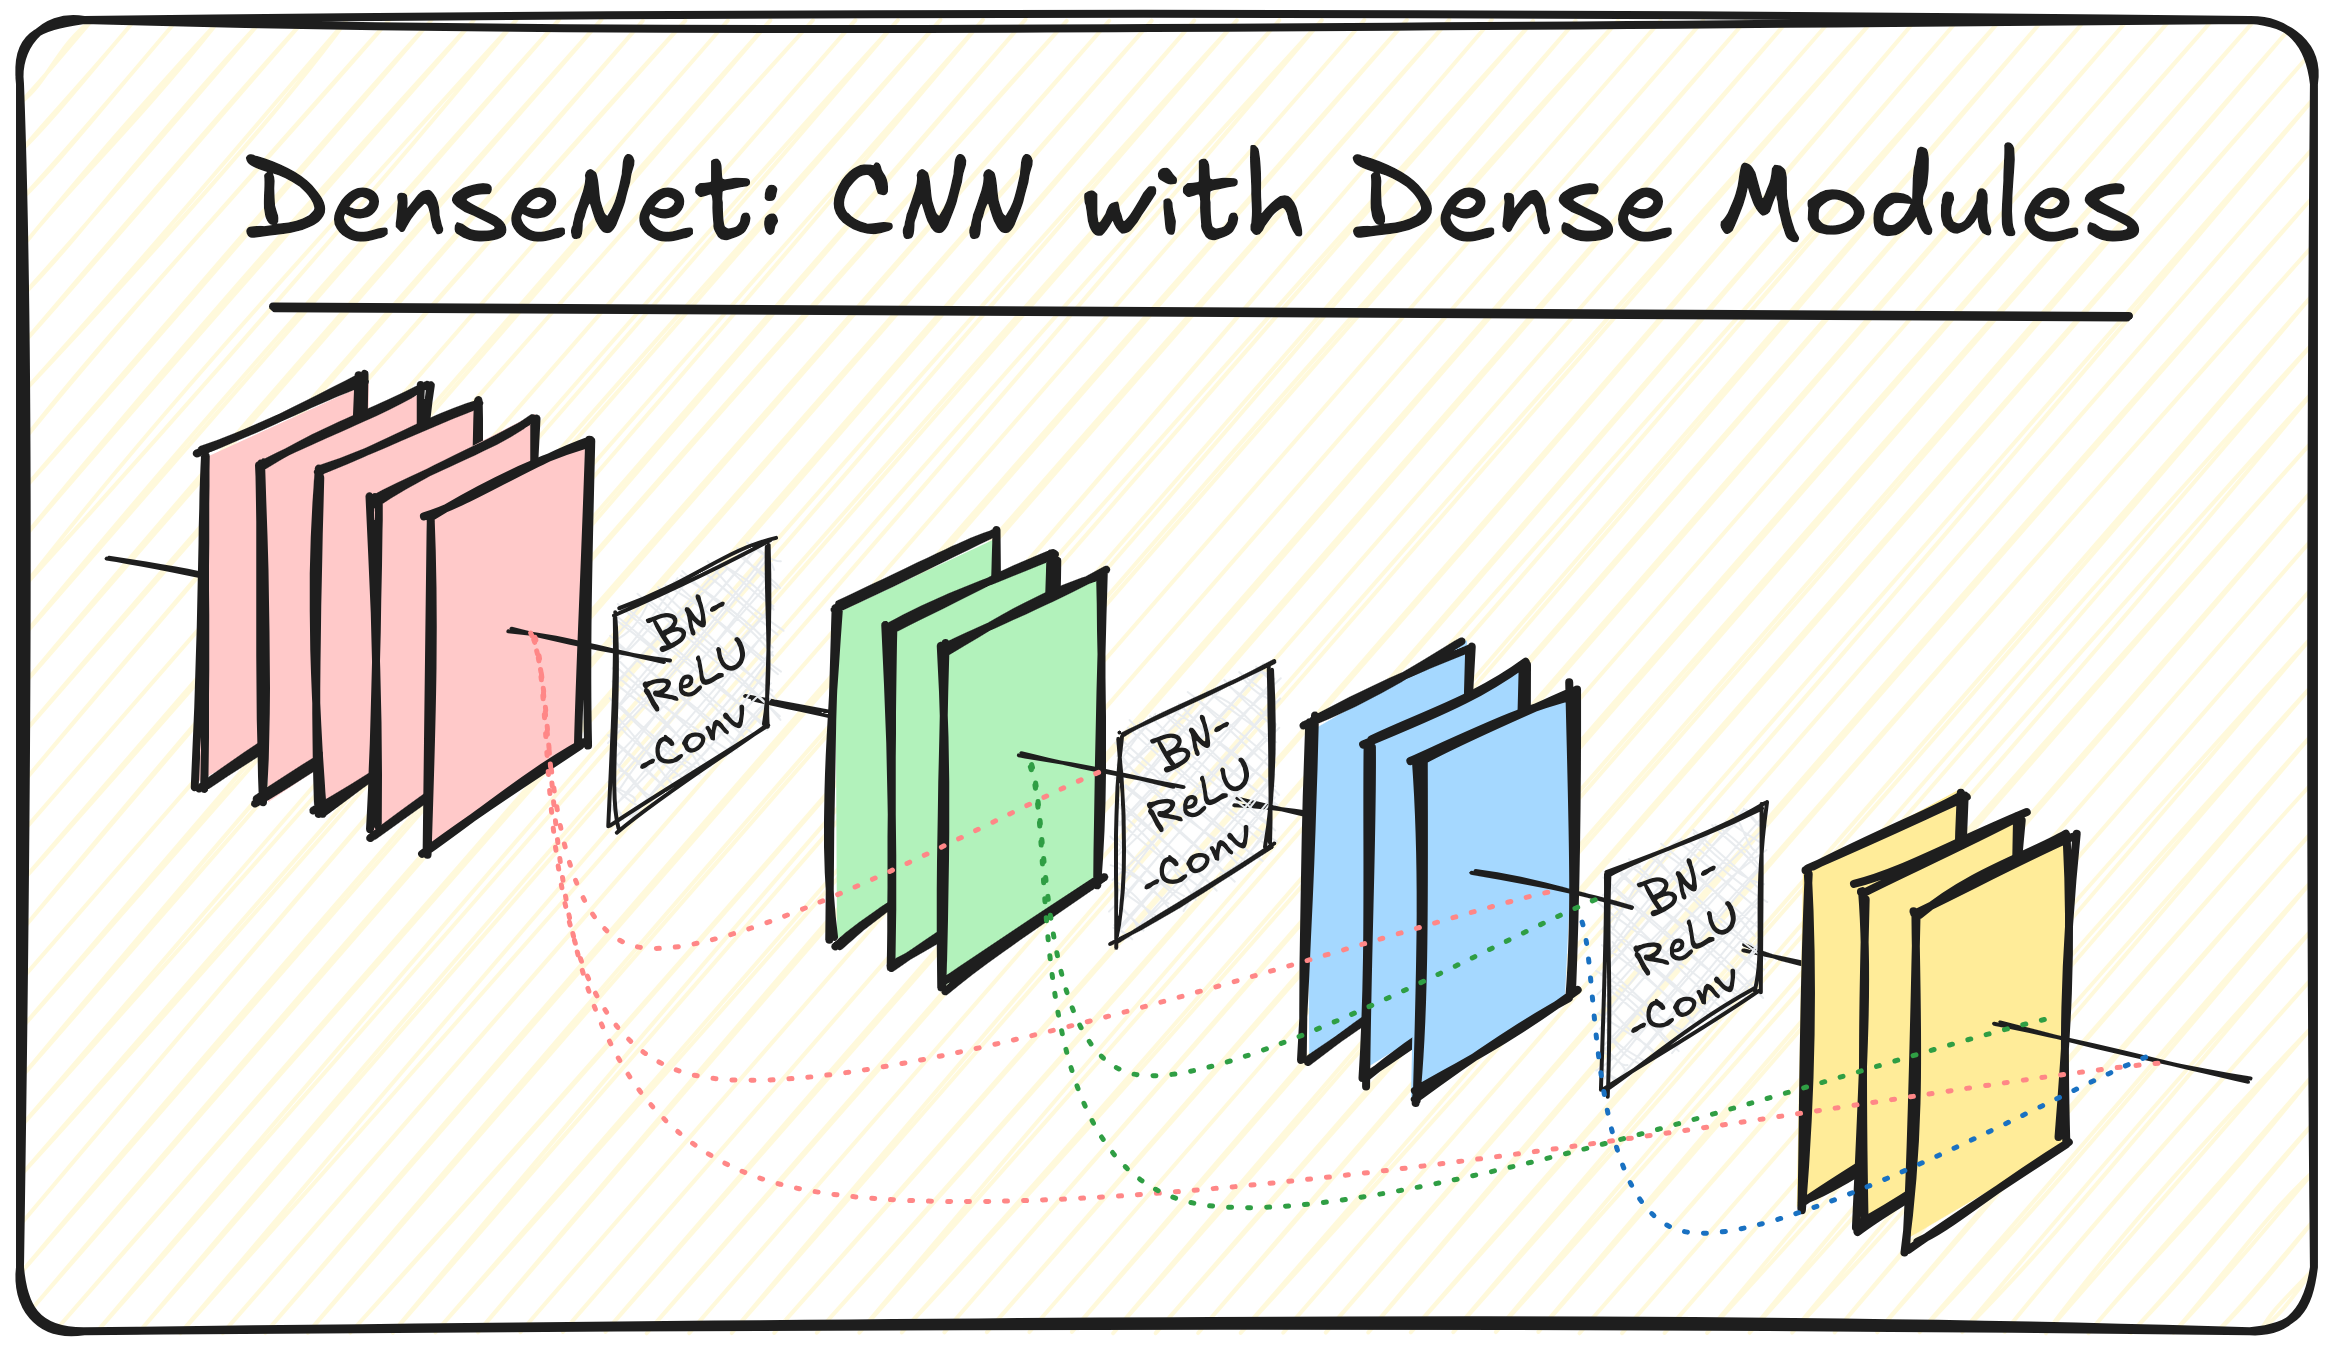
\includegraphics[width=\textwidth]{densenet-explanation.png}
\caption{DenseNet: dense (concatenating) blocks.}
\end{subfigure}
\caption{Conceptual illustration of the two transfer-learning backbones.
(a) ResNet adds a block's input to its output via skip connections (the image
restoration example is illustrative only). (b) DenseNet concatenates each
layer's output with all earlier feature maps. Figures adapted from the Vizuara
explainers~\cite{ref_vizuara_resnet,ref_vizuara_densenet}.}
\label{fig:architectures}
\end{figure}

\subsection{Training Protocol}

The custom CNN is trained from scratch for up to 20 epochs. The
transfer-learning models follow a two-phase schedule. In
\emph{phase 1} the backbone is frozen and only the new head is trained for
5 epochs, which adapts the classifier to the new label space without
destroying the pretrained features. In \emph{phase 2} the entire network
is unfrozen and fine-tuned for up to 30 additional epochs.

All models are optimised with Adam (learning rate $10^{-4}$) and a batch
size of 32. The binary task uses binary cross-entropy with logits; the
three-class task uses categorical cross-entropy. We use a
\texttt{ReduceLROnPlateau} scheduler (factor $0.5$, patience 3) on the
validation loss and early stopping (patience 5). The checkpoint with the
lowest validation loss is retained. To assess robustness, every model is
trained with three random seeds ($0$, $1$, $2$), and results are reported
as mean\,$\pm$\,standard deviation. All models are implemented in
PyTorch~\cite{ref_pytorch}, and metrics are computed with
scikit-learn~\cite{ref_scikit}.

\subsection{Ensemble}

We additionally build a simple ensemble that averages the predicted
probabilities of all six transfer-learning checkpoints (ResNet18 and
DenseNet121, each with three seeds). For the binary task this averages the
sigmoid outputs; for the three-class task it averages the softmax vectors.
The averaged probabilities are then thresholded (binary) or
\texttt{argmax}-ed (three-class) to obtain the final prediction.

\subsection{Calibration and Threshold Optimisation}

Beyond accuracy, we assess whether the predicted probabilities are
trustworthy. We compute the Expected Calibration Error
(ECE)~\cite{ref_calibration} with ten equal-width confidence bins and plot
reliability diagrams (mean accuracy vs.\ mean confidence per bin). For the
binary task we also derive task-specific decision thresholds for two
clinical scenarios: a \emph{screening} scenario, in which we pick the
highest threshold that still guarantees at least $99\%$ recall on pneumonia
(prioritising sensitivity, since missing a sick child is costly), and an
\emph{assisted-diagnosis} scenario, in which we pick the threshold that
maximises F1 (balancing precision and recall).

\subsection{Visual Explanations}

We use Grad-CAM~\cite{ref_gradcam} to produce class-discriminative
heatmaps from the last convolutional layer of each transfer-learning
model. These overlays let us qualitatively verify that correct predictions
are driven by lung-field opacities rather than by irrelevant image
artefacts, and they help to interpret failure cases.

\subsection{Evaluation Metrics}

For the binary task we report accuracy, precision, recall (sensitivity),
specificity, F1, and AUROC, together with the inference time per image.
For the three-class task we report accuracy, macro-averaged precision,
recall, and F1, per-class F1, and one-vs-rest macro AUROC. We emphasise
recall on the disease classes because, in a clinical context, false
negatives are more costly than false positives.

\section{Results}

\subsection{Training Dynamics}

Figure~\ref{fig:curves} shows the binary DenseNet121 training curves for
all three seeds. The two-phase schedule is clearly visible: training loss
falls rapidly and smoothly, while validation loss is noisier and plateaus
early, after which early stopping halts training (between epochs 11 and 23
depending on the seed). The validation F1 quickly saturates near $1.0$ on
the tiny 16-image validation split, which confirms that this split is too
small for reliable model selection and motivates reporting all final
numbers on the full 624-image test set instead. The custom CNN, by
contrast, exhibited markedly less stable validation behaviour across seeds,
foreshadowing the high variance reported below.

\begin{figure}[t]
\centering
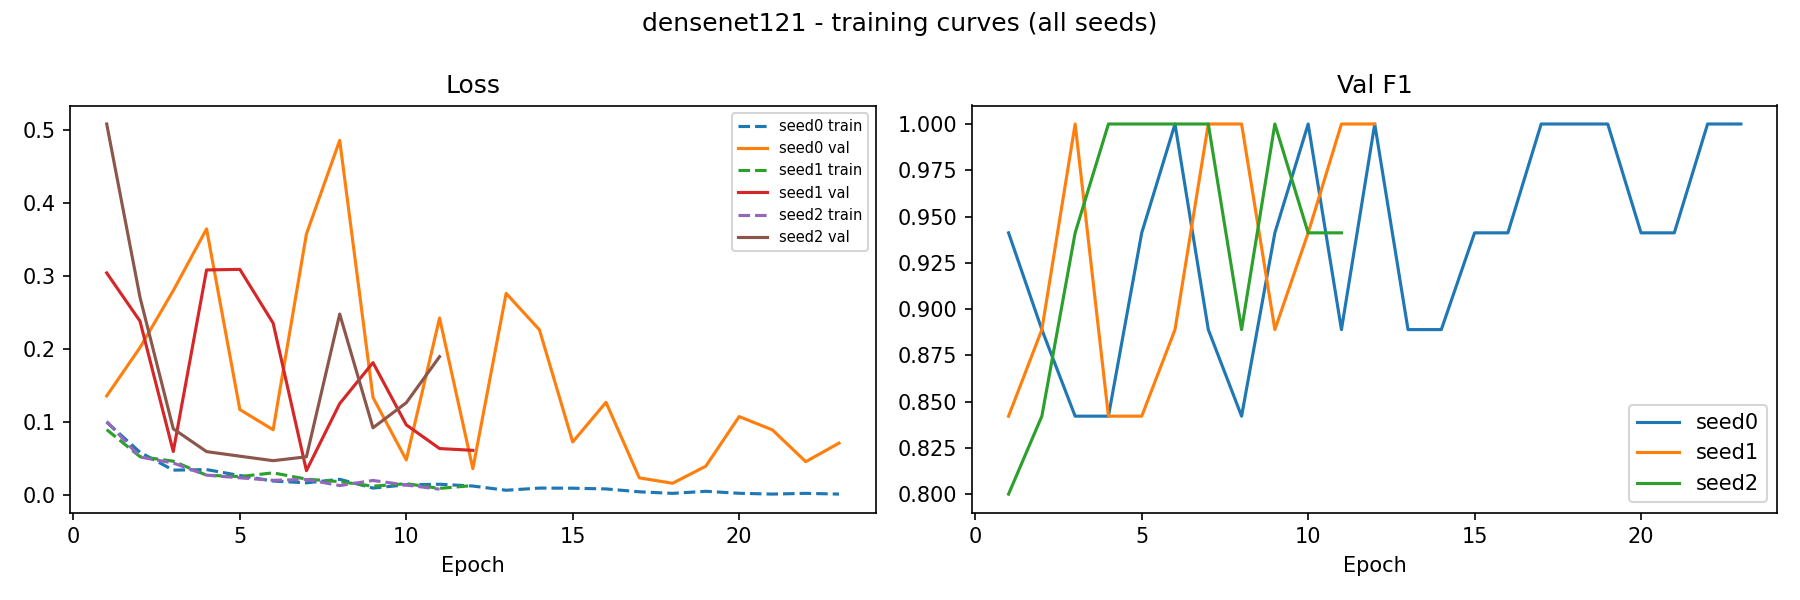
\includegraphics[width=\textwidth]{densenet121_training_curves.png}
\caption{Binary DenseNet121 training curves across the three seeds.
\emph{Left:} train (dashed) and validation (solid) loss; the train loss
converges smoothly while the validation loss is noisy on the small
validation set. \emph{Right:} validation F1 saturates near $1.0$, showing
the validation split is too small to discriminate between checkpoints.}
\label{fig:curves}
\end{figure}

\subsection{Binary Classification}

Table~\ref{tab:binary} reports the binary results across three seeds, and
Fig.~\ref{fig:metricbin} visualises the comparison. Both transfer-learning
models clearly outperform the custom CNN on every aggregate metric.
DenseNet121 is the strongest single model (accuracy $0.841$, F1 $0.887$,
AUROC $0.966$), narrowly ahead of ResNet18. The custom CNN reaches a
competitive F1 but is far less stable---its specificity varies enormously
across seeds ($0.494\pm0.359$)---showing that a from-scratch model on this
imbalanced data is highly sensitive to initialisation.

\begin{table}[!ht]
\caption{Binary classification (NORMAL vs.\ PNEUMONIA) on the test set,
mean\,$\pm$\,std over seeds $\{0,1,2\}$. The ensemble averages the six
transfer-learning checkpoints. Best value per column in \textbf{bold}.}
\label{tab:binary}
\centering
\setlength{\tabcolsep}{4pt}
\begin{tabular}{lcccccc}
\toprule
Model & Acc. & Prec. & Recall & Spec. & F1 & AUROC \\
\midrule
Custom CNN  & 0.756 & 0.768 & 0.914 & 0.494 & 0.828 & 0.886 \\
ResNet18    & 0.830 & 0.791 & 0.991 & 0.561 & 0.879 & 0.949 \\
DenseNet121 & 0.841 & 0.799 & \textbf{0.997} & \textbf{0.581} & 0.887 & \textbf{0.966} \\
\textbf{Ensemble} & \textbf{0.856} & \textbf{0.814} & \textbf{0.997} & 0.620 & \textbf{0.896} & 0.963 \\
\bottomrule
\end{tabular}
\end{table}

\begin{figure}[t]
\centering
\begin{subfigure}{0.62\textwidth}
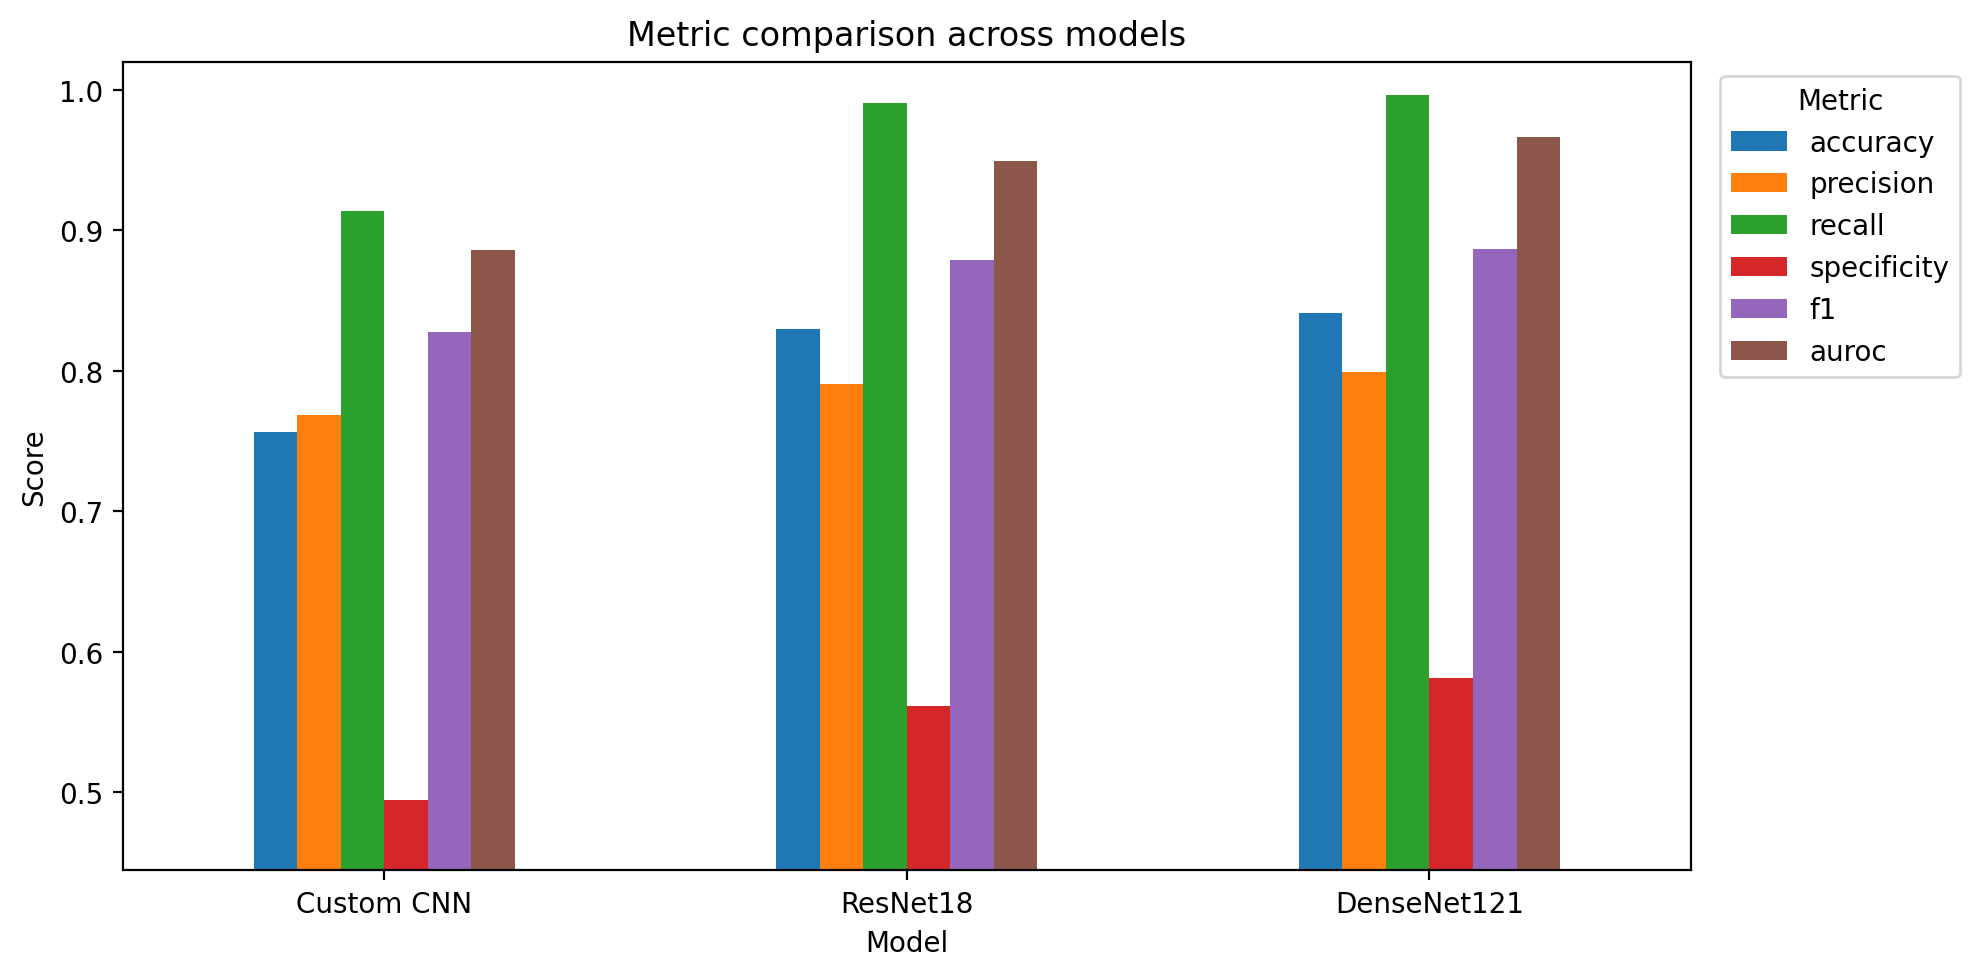
\includegraphics[width=\textwidth]{metric_comparison_binary.png}
\caption{Per-metric comparison}
\label{fig:metricbin}
\end{subfigure}\hfill
\begin{subfigure}{0.36\textwidth}
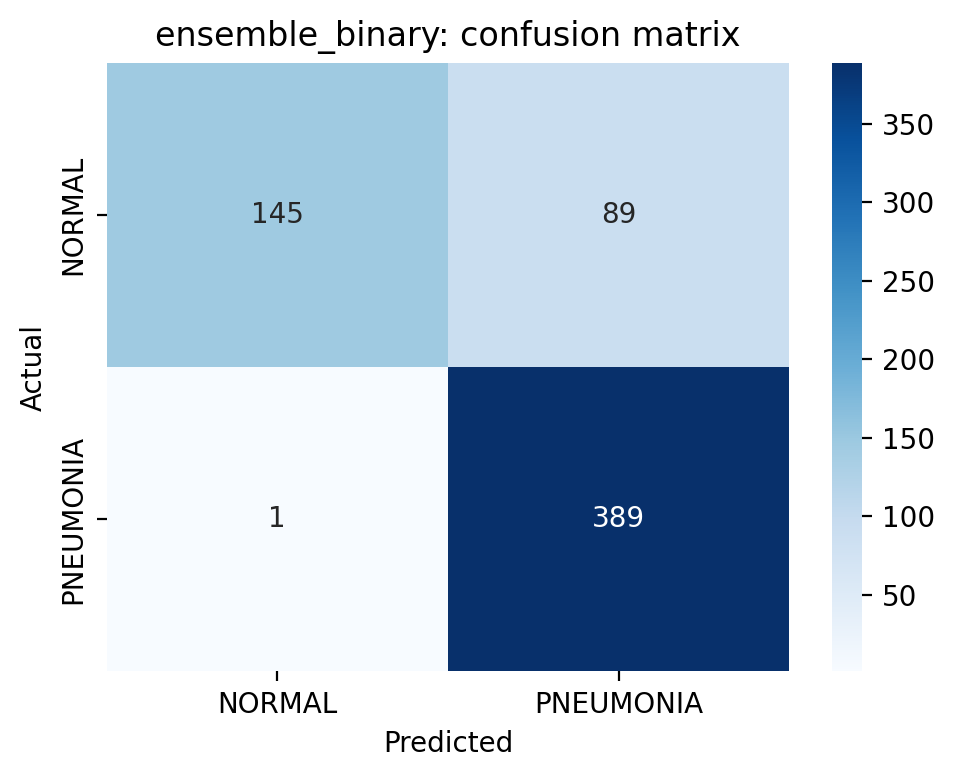
\includegraphics[width=\textwidth]{ensemble_binary_confusion_matrix.png}
\caption{Ensemble confusion matrix}
\label{fig:cmbin}
\end{subfigure}
\caption{Binary results. (a) All models share the same profile: very high
recall but comparatively low specificity (red bars). (b) The ensemble
misses only $1$ of $390$ pneumonia cases (FN), at the cost of $89$ false
positives on NORMAL.}
\label{fig:binary}
\end{figure}

The ensemble gives the best overall trade-off (accuracy $0.856$, F1 $0.896$,
recall $0.997$), missing only $1$ of the $390$ pneumonia cases
(Fig.~\ref{fig:cmbin}: TN$=145$, FP$=89$, FN$=1$, TP$=389$). The recurring
weakness is specificity: the models eagerly predict pneumonia and mislabel a
fair share of normal images. This is the expected---and for a screening tool
arguably desirable---bias, since a missed pneumonia is more dangerous than a
false alarm, but it leaves room for improvement on the NORMAL class.

\subsection{Three-Class Classification}

Table~\ref{tab:threeclass} reports the three-class results and
Fig.~\ref{fig:metric3class} visualises them. As expected, separating
bacterial from viral pneumonia is substantially harder than the binary
task. To obtain trustworthy estimates we use a \emph{patient-aware}
stratified validation split: because the Kermany dataset contains several
images per patient, an image-level split leaks the same patient across
train and validation and inflates the reported scores. Holding out whole
patients instead, together with inverse-frequency class weights and
checkpoint selection by macro-F1, yields a more conservative but honest
DenseNet121 macro-F1 of $0.784$ (vs.\ ResNet18 $0.751$). The ensemble of
both backbones gives the best result, reaching an accuracy of $0.822$, a
macro-F1 of $0.808$, and a one-vs-rest AUROC of $0.960$.

We also evaluated a \emph{hierarchical} two-stage variant inspired by
Kermany et al.~\cite{ref_kermany}, in which the binary NORMAL-vs-PNEUMONIA
model is followed by a dedicated bacteria-vs-virus classifier trained only
on pneumonia images. This did not outperform the flat three-way softmax
(macro-F1 $0.774$ vs.\ $0.784$; AUROC $0.944$ for both), confirming that the
viral/bacterial boundary -- not the pipeline structure -- is the intrinsic
bottleneck.

\begin{table}[!ht]
\caption{Three-class classification (NORMAL / BACTERIA / VIRUS) on the
test set, mean\,$\pm$\,std over seeds $\{0,1,2\}$ (single models) or
deterministic for the ensemble. Macro-averaged metrics. Best in
\textbf{bold}.}
\label{tab:threeclass}
\centering
\setlength{\tabcolsep}{4pt}
\resizebox{\textwidth}{!}{%
\begin{tabular}{lccccc}
\toprule
Model & Acc. & Prec.$_\text{M}$ & Recall$_\text{M}$ & F1$_\text{M}$ & AUROC \\
\midrule
ResNet18    & $0.769\pm0.089$ & $0.805\pm0.037$ & $0.777\pm0.077$ & $0.751\pm0.099$ & $0.944\pm0.019$ \\
DenseNet121 & $0.799\pm0.029$ & $0.808\pm0.024$ & $0.796\pm0.033$ & $0.784\pm0.033$ & $0.944\pm0.012$ \\
DenseNet121 (hierarchical) & $0.790\pm0.019$ & $0.808\pm0.010$ & $0.794\pm0.016$ & $0.774\pm0.021$ & $0.944\pm0.002$ \\
\textbf{Ensemble} & \textbf{0.822} & \textbf{0.831} & \textbf{0.824} & \textbf{0.808} & \textbf{0.960} \\
\bottomrule
\end{tabular}}
\end{table}

\begin{figure}[t]
\centering
\begin{subfigure}{0.52\textwidth}
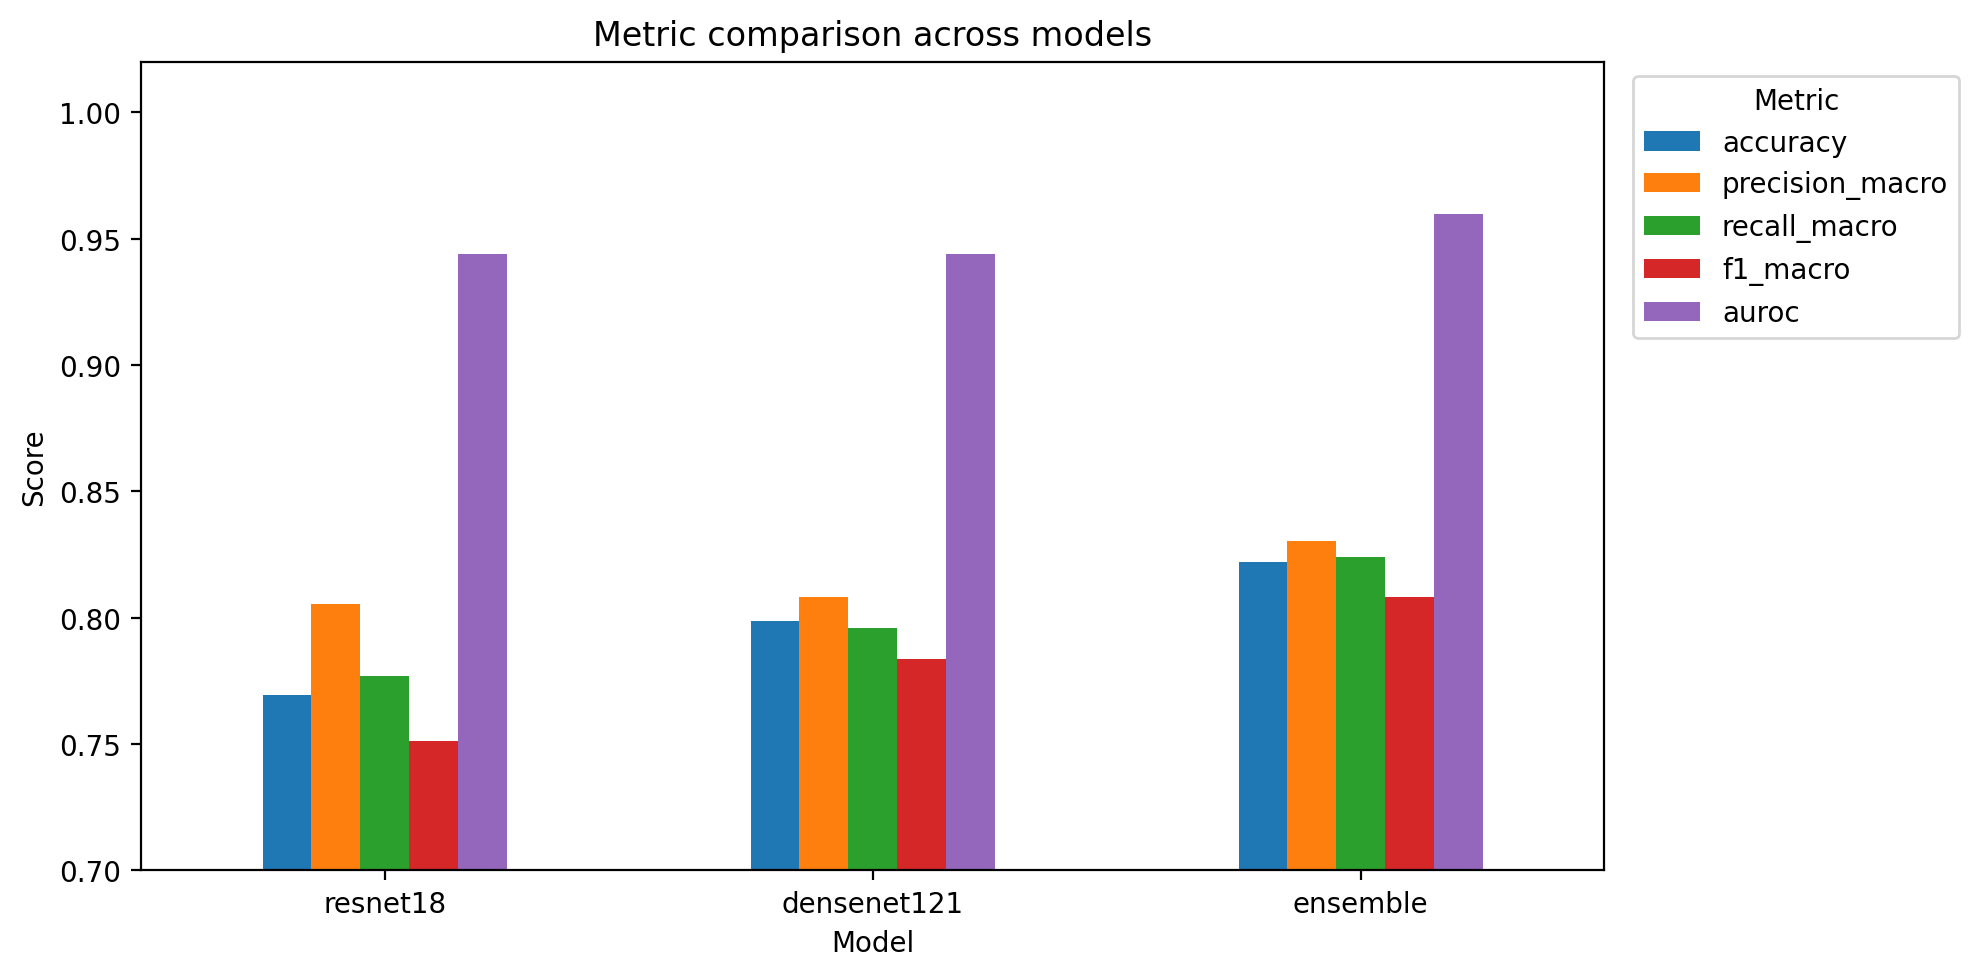
\includegraphics[width=\textwidth]{metric_comparison_3class.png}
\caption{Per-metric comparison}
\label{fig:metric3class}
\end{subfigure}\hfill
\begin{subfigure}{0.46\textwidth}
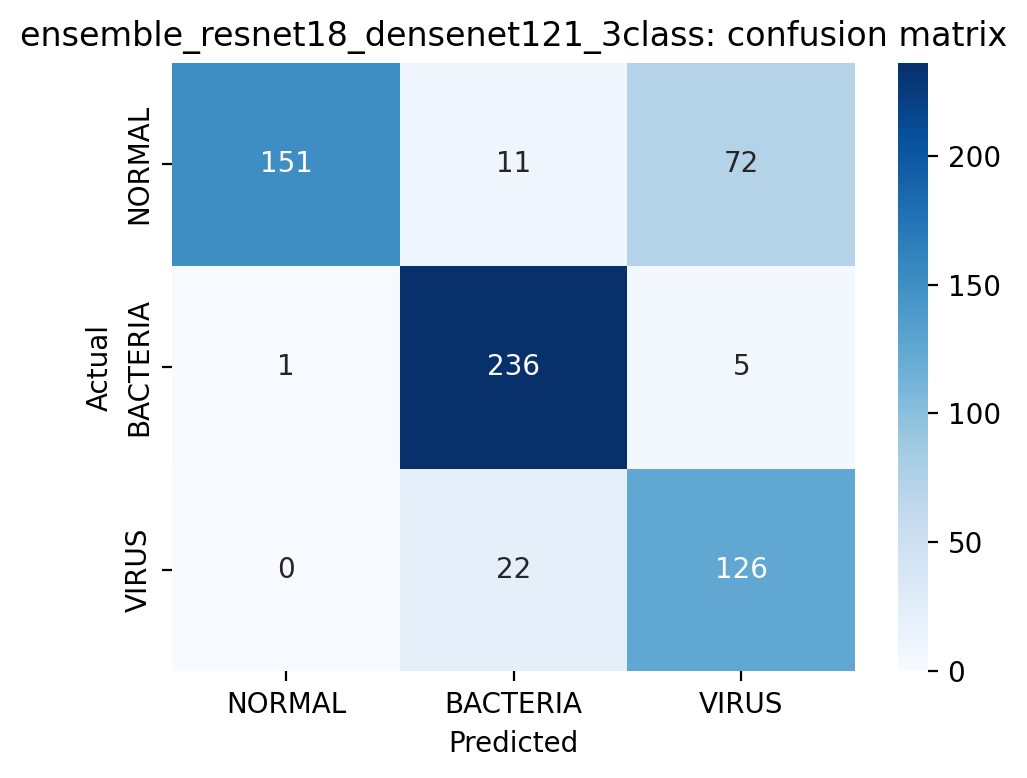
\includegraphics[width=\textwidth]{ensemble_resnet18_densenet121_3class_confusion_matrix.png}
\caption{Ensemble confusion matrix}
\label{fig:cm3class}
\end{subfigure}
\caption{Three-class results. (a) DenseNet121 and the ensemble dominate
ResNet18 on every macro-averaged metric. (b) The dominant error is $72$
NORMAL images predicted as VIRUS; BACTERIA is recognised almost perfectly.}
\label{fig:threeclass}
\end{figure}

\subsection{Error Analysis}

The per-class breakdown of the ensemble is the most informative result.
Table~\ref{tab:perclass} reports per-class precision, recall, and F1, and
Fig.~\ref{fig:cm3class} shows the confusion matrix.

\begin{table}[!ht]
\caption{Per-class metrics of the three-class ensemble on the test set.}
\label{tab:perclass}
\centering
\setlength{\tabcolsep}{8pt}
\begin{tabular}{lcccc}
\toprule
Class & Precision & Recall & F1 & Support \\
\midrule
NORMAL   & 0.993 & 0.645 & 0.782 & 234 \\
BACTERIA & 0.877 & 0.975 & 0.924 & 242 \\
VIRUS    & 0.621 & 0.851 & 0.718 & 148 \\
\bottomrule
\end{tabular}
\end{table}

First, \textbf{bacterial pneumonia is recognised very reliably}
(F1 $0.924$, recall $0.975$): it is the majority class and the most
visually distinctive, producing dense, lobar consolidation. Second,
\textbf{viral pneumonia is the hardest class} (F1 $0.718$): its diffuse,
interstitial pattern is easily confused with both normal lungs and early
bacterial infiltrates, which is reflected in its low precision ($0.621$).
Third, and most striking, \textbf{the dominant error mode is the
NORMAL$\rightarrow$VIRUS confusion}: $72$ of the $234$ NORMAL images are
predicted as VIRUS, which is why NORMAL recall ($0.645$) is the lowest of the
three classes despite NORMAL precision being the highest ($0.993$). The model
almost never calls a sick lung normal (only $1$ BACTERIA and $0$ VIRUS images
are misread as NORMAL), but it sometimes reads a faint normal lung as viral
pneumonia---a conservative, screening-friendly direction of error that mirrors
the clinical difficulty of distinguishing subtle viral infiltrates from normal
vascular markings.

\subsection{Inference Cost}

All models are lightweight at inference: per-image time ranges from
$\approx12.6$\,ms (ResNet18) to $\approx15.1$\,ms (DenseNet121), i.e.\
$60$--$80$ images/s on a single GPU. The custom CNN is no faster than the
transfer-learning models, so its lower accuracy buys no speed advantage---a
further reason to prefer the pretrained backbones.

\subsection{Calibration and Decision Thresholds}\label{sec:calib}

Table~\ref{tab:calibration} reports the calibration analysis. The
from-scratch custom CNN is, perhaps surprisingly, the best-calibrated binary
model (ECE $0.108$), whereas the transfer-learning models are overconfident
(ECE $0.153$--$0.160$), pushing probabilities towards the extremes. The
three-class models are less calibrated still (ECE $0.245$--$0.276$),
reflecting the harder task. The reliability diagrams
(Fig.~\ref{fig:reliability}, Appendix) confirm that the transfer-learning
models concentrate predictions in the high-confidence bins, far from the
diagonal.

\begin{table}[!ht]
\caption{Expected Calibration Error (ECE, 10 bins, lower is better) and
optimised binary decision thresholds. ``Screening'' is the highest
threshold maintaining $\geq99\%$ recall; ``F1'' maximises F1. Thresholds
are only defined for the binary task.}
\label{tab:calibration}
\centering
\setlength{\tabcolsep}{6pt}
\begin{tabular}{lccc}
\toprule
Model & ECE & Thr.\ (screening) & Thr.\ (F1) \\
\midrule
Custom CNN              & $0.108\pm0.051$ & 0.245 & 0.596 \\
ResNet18                & $0.160\pm0.016$ & 0.593 & 0.981 \\
DenseNet121             & $0.153\pm0.015$ & 0.860 & 0.995 \\
Ensemble (binary)       & $0.156$         & 0.751 & 0.986 \\
ResNet18 (3-class)      & $0.266\pm0.086$ & --    & --    \\
DenseNet121 (3-class)   & $0.245\pm0.027$ & --    & --    \\
Ensemble (3-class)      & $0.276$         & --    & --    \\
\bottomrule
\end{tabular}
\end{table}

The threshold analysis quantifies an operational point. Because the
transfer-learning models are confident, the default $0.5$ threshold is not
optimal: maximising F1 requires very high thresholds (e.g.\ $0.995$ for
DenseNet121), whereas a screening deployment demanding $\geq99\%$ recall can
afford a much lower one. Exposing both operating points makes the same
trained model usable in a high-sensitivity triage mode and a balanced
assisted-diagnosis mode, without retraining.

\subsection{Grad-CAM Visual Explanations}

Figure~\ref{fig:gradcam} collects DenseNet121 Grad-CAM overlays for both
tasks. On the binary task (top row), true positives and true negatives are
anatomically sensible---activation concentrates on the consolidated lung
field for pneumonia and is diffuse/peripheral for normal lungs---whereas the
false positive and false negative reveal where the model is led astray. The
three-class row (bottom) extends this: correct bacterial and normal
predictions focus on the relevant regions, while the
NORMAL$\rightarrow$VIRUS failure shows diffuse activation over otherwise
normal lungs, visually corroborating the dominant error mode identified in
Table~\ref{tab:perclass}.

\begin{figure}[H]
\centering
\begin{subfigure}{0.21\textwidth}
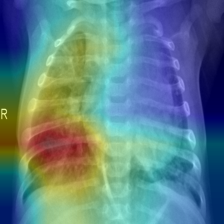
\includegraphics[width=\textwidth]{densenet121_true_positive_pneumonia_person100_bacteria_4.png}
\caption{TP (pneumonia)}
\end{subfigure}\hfill
\begin{subfigure}{0.21\textwidth}
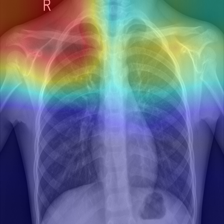
\includegraphics[width=\textwidth]{densenet121_true_negative_normal_IM-0001-0001.png}
\caption{TN (normal)}
\end{subfigure}\hfill
\begin{subfigure}{0.21\textwidth}
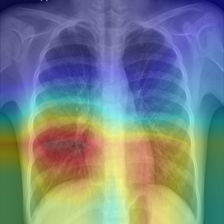
\includegraphics[width=\textwidth]{densenet121_false_positive_normal_IM-0019-0001.png}
\caption{FP (binary)}
\end{subfigure}\hfill
\begin{subfigure}{0.21\textwidth}
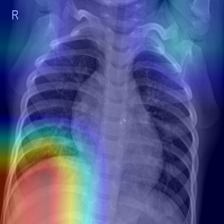
\includegraphics[width=\textwidth]{densenet121_false_negative_pneumonia_person154_bacteria_7.png}
\caption{FN (binary)}
\end{subfigure}

\vspace{0.3em}
\begin{subfigure}{0.21\textwidth}
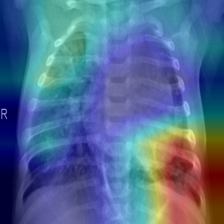
\includegraphics[width=\textwidth]{densenet121_3class_correct_BACTERIA_person100_bacteria_4.png}
\caption{Correct: BACTERIA}
\end{subfigure}\hfill
\begin{subfigure}{0.21\textwidth}
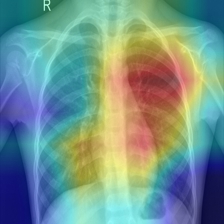
\includegraphics[width=\textwidth]{densenet121_3class_correct_NORMAL_IM-0001-0001.png}
\caption{Correct: NORMAL}
\end{subfigure}\hfill
\begin{subfigure}{0.21\textwidth}
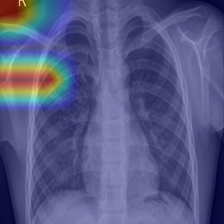
\includegraphics[width=\textwidth]{densenet121_3class_wrong_NORMAL_as_VIRUS_IM-0015-0001.png}
\caption{Error: NORMAL$\rightarrow$VIRUS}
\end{subfigure}\hfill
\begin{subfigure}{0.21\textwidth}
\phantom{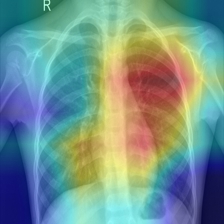
\includegraphics[width=\textwidth]{densenet121_3class_correct_NORMAL_IM-0001-0001.png}}
\end{subfigure}
\caption{DenseNet121 Grad-CAM overlays. \emph{Top:} the four binary outcome
types; correct predictions (TP, TN) attend to plausible lung regions, the FP
and FN illustrate the failure modes behind the imperfect specificity.
\emph{Bottom:} three-class examples; correct BACTERIA/NORMAL predictions
focus on the relevant regions, while the NORMAL$\rightarrow$VIRUS case shows
diffuse activation over an otherwise normal lung---the dominant error mode.
No clean correctly-classified VIRUS example exists, consistent with viral
pneumonia being the hardest class.}
\label{fig:gradcam}
\end{figure}

\section{Discussion}

Three findings stand out. First, transfer learning is decisively better
than training from scratch: ResNet18 and DenseNet121 outperform the custom
CNN on every metric and are far more stable across seeds, so ImageNet
features are a strong and cheap prior given limited medical data. Second, the
three-class extension is both feasible and informative. Accuracy drops
relative to the binary task (as expected), but the model still separates
bacterial from viral pneumonia well above chance, and the per-class analysis
localises the difficulty precisely at the NORMAL/VIRUS boundary, mirroring
the known clinical difficulty of distinguishing viral infiltrates from normal
variation. Third, the auxiliary analyses---ensembling, calibration, and
threshold optimisation---turn a raw classifier into something closer to a
deployable component, reducing variance, exposing over-confidence, and giving
explicit operating points for screening versus assisted diagnosis.

\paragraph{Limitations.}
Several caveats apply. (i) The data comes from a single centre and a narrow
pediatric age range, so generalisation to other populations or acquisition
protocols is unproven. (ii) The validation split is tiny, making model
selection noisy; re-sampling mitigated but did not remove this. (iii) The
bacterial/viral labels inherit the dataset's original (possibly imperfect)
labelling. (iv) Class imbalance was not corrected beyond augmentation, which
partly explains the low specificity. (v) All metrics are on a single test
set; external validation is needed before any real-world claim. The system
is for educational use only and is not a diagnostic device.

\section{Conclusion and Future Work}

We presented a reproducible study of deep-learning models for pediatric
pneumonia classification, progressing from a binary baseline to a
clinically motivated three-class extension that distinguishes bacterial
from viral pneumonia. Transfer-learning backbones, and especially a simple
ensemble of ResNet18 and DenseNet121, gave the best results: an F1 of
$0.896$ and $99.7\%$ pneumonia recall on the binary task, and a macro-F1 of
$0.808$ on the three-class task (evaluated with a leakage-free patient-aware
split). A hierarchical two-stage variant did not improve on the flat
softmax, indicating that the viral/bacterial distinction is an intrinsic
limit rather than a modelling artefact. Calibration, threshold optimisation,
and Grad-CAM analyses added interpretability and operational flexibility.

Future work includes addressing class imbalance with weighted or focal
loss~\cite{ref_focal}, temperature scaling~\cite{ref_calibration} for
calibration, stronger backbones and test-time augmentation, and---most
importantly---external validation on independent CXR datasets. All code,
configurations, and scripts needed to reproduce every number and figure are
released in the accompanying repository, and the trained model weights are
published on the Hugging Face Hub at
\url{https://huggingface.co/luanacarolina/pneumonia-chest-xray-classifier}.

\newpage

%
% ---- Bibliography ----
%
\begin{thebibliography}{20}

% --- References carried over from the project proposal report ---

\bibitem{ref_resnet}
He, K., Zhang, X., Ren, S., Sun, J.: Deep residual learning for image
recognition. In: Proceedings of the IEEE Conference on Computer Vision and
Pattern Recognition (CVPR), pp. 770--778. IEEE, Las Vegas, NV, USA (2016).
\url{https://openaccess.thecvf.com/content_cvpr_2016/html/He_Deep_Residual_Learning_CVPR_2016_paper.html}

\bibitem{ref_densenet}
Huang, G., Liu, Z., van der Maaten, L., Weinberger, K.Q.: Densely connected
convolutional networks. In: Proceedings of the IEEE Conference on Computer
Vision and Pattern Recognition (CVPR), pp. 4700--4708. IEEE, Honolulu, HI,
USA (2017).
\url{https://openaccess.thecvf.com/content_cvpr_2017/html/Huang_Densely_Connected_Convolutional_CVPR_2017_paper.html}

\bibitem{ref_kermany}
Kermany, D.S., Goldbaum, M., Cai, W., Valentim, C.C.S., Liang, H., Baxter,
S.L., McKeown, A., Yang, G., Wu, X., Yan, F., Dong, J., Prasadha, M., Pei,
J., Ting, M., Zhu, J., Li, C., Hewett, S., Dong, J., Sun, I., Wang, J.,
Clark, K.J., Brown, S.M., Ostmo, A., Wilson, C.S., Zhang, K.: Identifying
medical diagnoses and treatable diseases by image-based deep learning.
Cell \textbf{172}(5), 1122--1131 (2018). \doi{10.1016/j.cell.2018.02.010}

\bibitem{ref_kaggle}
Mooney, P.: Chest X-Ray Images (Pneumonia). Kaggle (2018). Original data from
Kermany et al. (2018).
\url{https://www.kaggle.com/datasets/paultimothymooney/chest-xray-pneumonia},
last accessed 2026-03-29

\bibitem{ref_chexnet}
Rajpurkar, P., Irvin, J., Zhu, K., Yang, B., Mehta, H., Duan, T., Ding, D.,
Bagul, A., Langlotz, C.P., Shpanskaya, K., Lungren, M.P., Ng, A.Y.: CheXNet:
Radiologist-level pneumonia detection on chest X-rays with deep learning.
arXiv preprint arXiv:1711.05225 (2017).
\url{https://arxiv.org/abs/1711.05225}

\bibitem{ref_gradcam}
Selvaraju, R.R., Cogswell, M., Das, A., Vedantam, R., Parikh, D., Batra, D.:
Grad-CAM: Visual explanations from deep networks via gradient-based
localization. In: Proceedings of the IEEE International Conference on
Computer Vision (ICCV), pp. 618--626. IEEE, Venice, Italy (2017).
\url{https://openaccess.thecvf.com/content_iccv_2017/html/Selvaraju_Grad-CAM_Visual_Explanations_ICCV_2017_paper.html}

% --- Additional references for the three-class extension and analyses ---

\bibitem{ref_chestxray14}
Wang, X., Peng, Y., Lu, L., Lu, Z., Bagheri, M., Summers, R.M.:
ChestX-ray8: Hospital-scale chest X-ray database and benchmarks on
weakly-supervised classification and localization of common thorax
diseases. In: IEEE CVPR, pp. 2097--2106 (2017).
\doi{10.1109/CVPR.2017.369}

\bibitem{ref_calibration}
Guo, C., Pleiss, G., Sun, Y., Weinberger, K.Q.: On calibration of modern
neural networks. In: Proceedings of the 34th International Conference on
Machine Learning (ICML), vol.~70, pp. 1321--1330 (2017)

\bibitem{ref_naeini}
Naeini, M.P., Cooper, G.F., Hauskrecht, M.: Obtaining well calibrated
probabilities using Bayesian binning. In: Proceedings of the 29th AAAI
Conference on Artificial Intelligence, pp. 2901--2907 (2015)

\bibitem{ref_focal}
Lin, T.-Y., Goyal, P., Girshick, R., He, K., Doll\'ar, P.: Focal loss for
dense object detection. In: IEEE ICCV, pp. 2980--2988 (2017).
\doi{10.1109/ICCV.2017.324}

\bibitem{ref_ensemble}
Dietterich, T.G.: Ensemble methods in machine learning. In: Multiple
Classifier Systems (MCS), LNCS, vol.~1857, pp. 1--15. Springer, Heidelberg
(2000). \doi{10.1007/3-540-45014-9_1}

\bibitem{ref_kundu}
Kundu, R., Das, R., Geem, Z.W., Han, G.-T., Sarkar, R.: Pneumonia detection
in chest X-ray images using an ensemble of deep learning models. PLOS ONE
\textbf{16}(9), e0256630 (2021). \doi{10.1371/journal.pone.0256630}

\bibitem{ref_rahman}
Rahman, T., Chowdhury, M.E.H., Khandakar, A., Islam, K.R., Islam, K.F.,
Mahbub, Z.B., Kadir, M.A., Kashem, S.: Transfer learning with deep
convolutional neural network (CNN) for pneumonia detection using chest
X-ray. Applied Sciences \textbf{10}(9), 3233 (2020).
\doi{10.3390/app10093233}

\bibitem{ref_imagenet}
Deng, J., Dong, W., Socher, R., Li, L.-J., Li, K., Fei-Fei, L.: ImageNet: A
large-scale hierarchical image database. In: IEEE CVPR, pp. 248--255
(2009). \doi{10.1109/CVPR.2009.5206848}

\bibitem{ref_alexnet}
Krizhevsky, A., Sutskever, I., Hinton, G.E.: ImageNet classification with
deep convolutional neural networks. In: Advances in Neural Information
Processing Systems (NeurIPS), vol.~25, pp. 1097--1105 (2012).
\doi{10.1145/3065386}

\bibitem{ref_pytorch}
Paszke, A., Gross, S., Massa, F., et al.: PyTorch: An imperative style,
high-performance deep learning library. In: NeurIPS, pp. 8024--8035 (2019)

\bibitem{ref_scikit}
Pedregosa, F., et al.: Scikit-learn: Machine learning in Python. Journal of
Machine Learning Research \textbf{12}, 2825--2830 (2011)

\bibitem{ref_vizuara_resnet}
Vizuara: ResNet --- The architecture that changed machine learning forever.
Vizuara Newsletter (2024).
\url{https://www.vizuaranewsletter.com/p/resnet-the-architecture-that-changed}

\bibitem{ref_vizuara_densenet}
Vizuara: DenseNet and EfficientNet are 1/20th the size of VGG16. Vizuara
Newsletter (2024).
\url{https://www.vizuaranewsletter.com/p/densenet-and-efficientnet-are-120th}
\end{thebibliography}

%
% ---- Appendix ----
%
\newpage
\section{Appendix: Per-Seed Training and Evaluation}

This appendix provides the full per-seed material that supports the
aggregated results in the main text. It is supplementary and does not count
towards the page limit.

\subsection{Reliability Diagrams}

Figure~\ref{fig:reliability} shows the reliability diagrams referenced in the
calibration analysis (Section~\ref{sec:calib}). The dashed diagonal is perfect
calibration; points above it indicate under-confidence and below it
over-confidence. The transfer-learning models concentrate their predictions
in the high-confidence bins, far from the diagonal, confirming the
over-confidence reported by the ECE values in Table~\ref{tab:calibration}.

\begin{figure}[h]
\centering
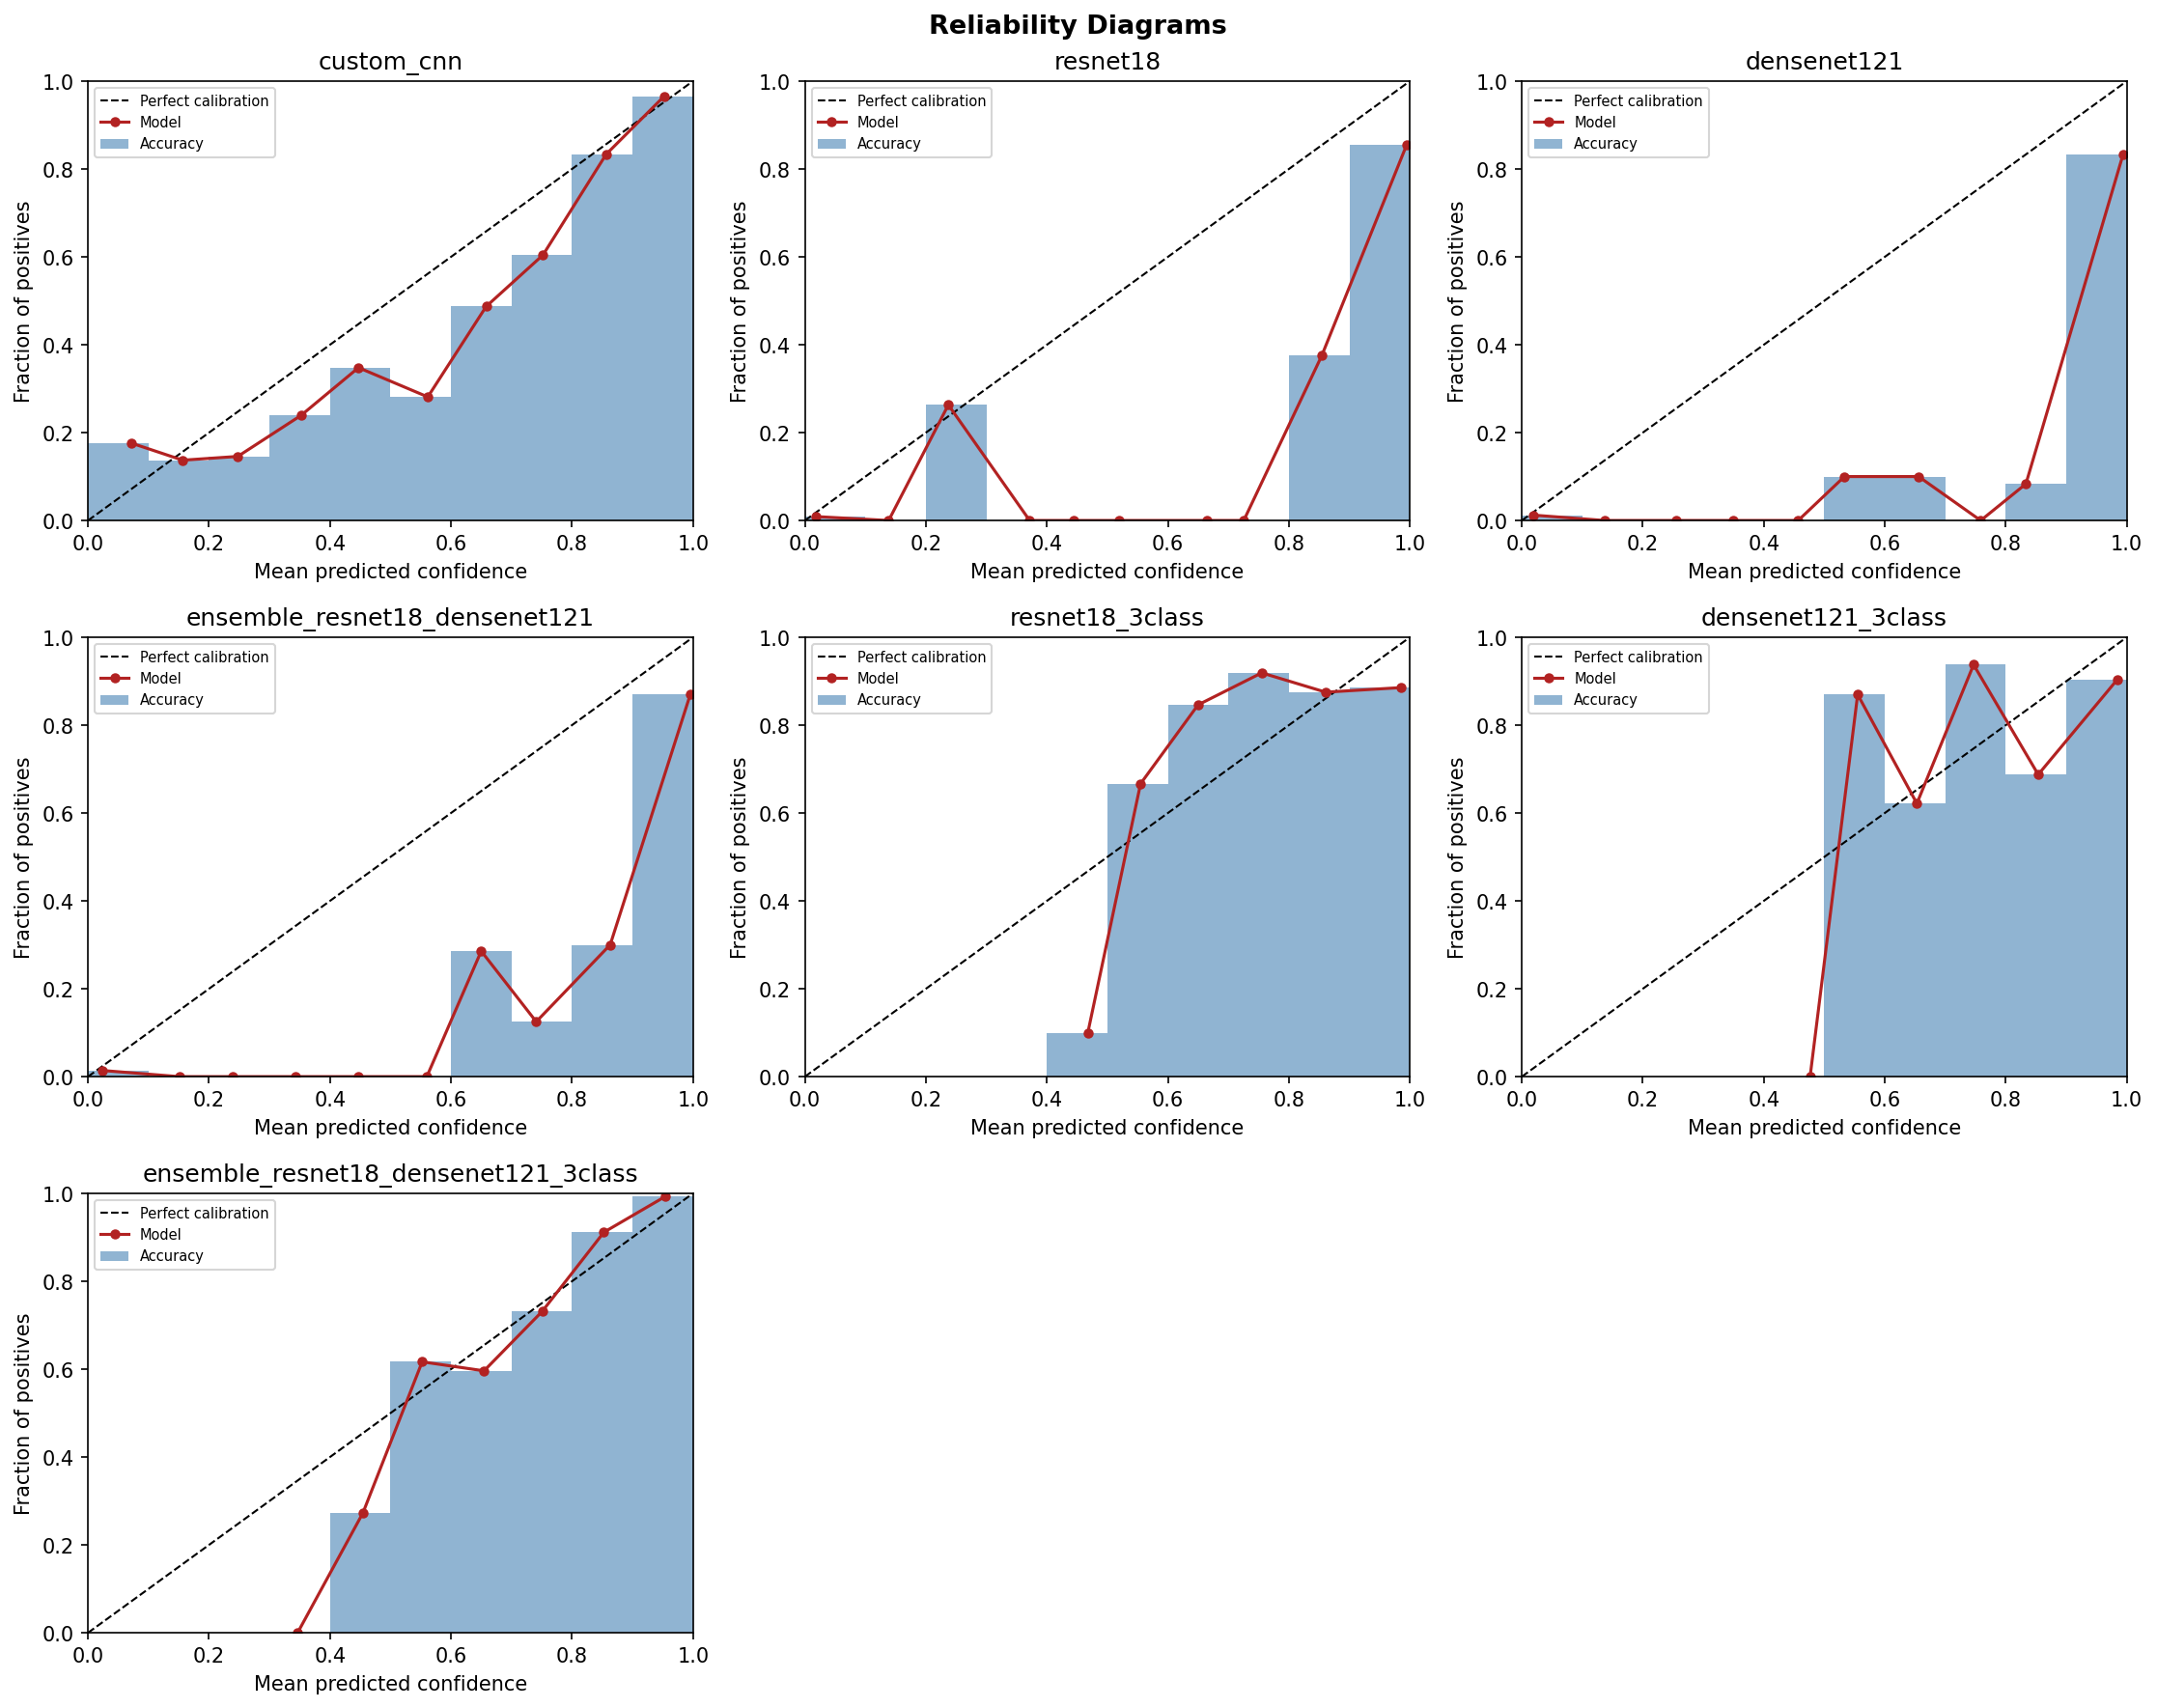
\includegraphics[width=0.9\textwidth]{reliability_diagrams.png}
\caption{Reliability diagrams for all models (binary and three-class).}
\label{fig:reliability}
\end{figure}

\FloatBarrier
\subsection{Three-Class Training Curves (per seed)}

Figure~\ref{fig:app_curves} shows the fine-tuning loss and validation-F1
curves for both backbones across the three seeds. DenseNet121 converges to
a lower and more stable validation loss than ResNet18, consistent with its
higher final accuracy.

\begin{figure}[h]
\centering
\begin{subfigure}{0.48\textwidth}
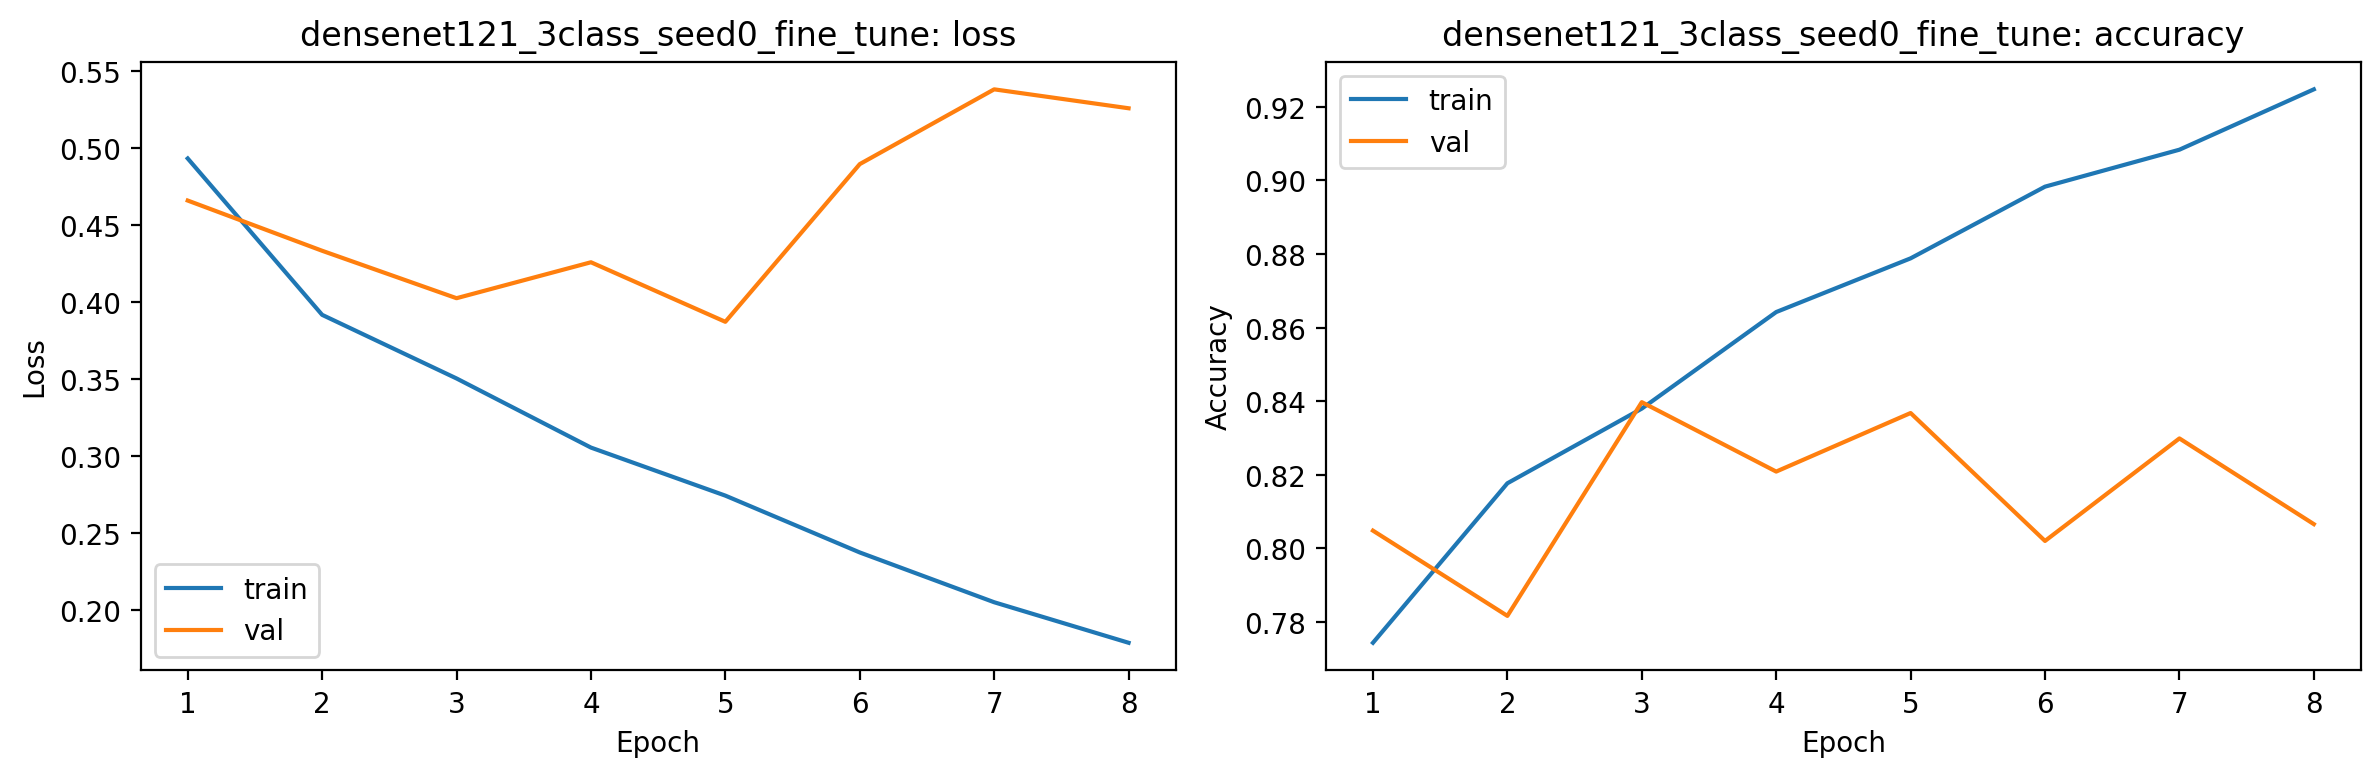
\includegraphics[width=\textwidth]{densenet121_3class_seed0_fine_tune_training_curves.png}
\caption{DenseNet121, seed 0}
\end{subfigure}\hfill
\begin{subfigure}{0.48\textwidth}
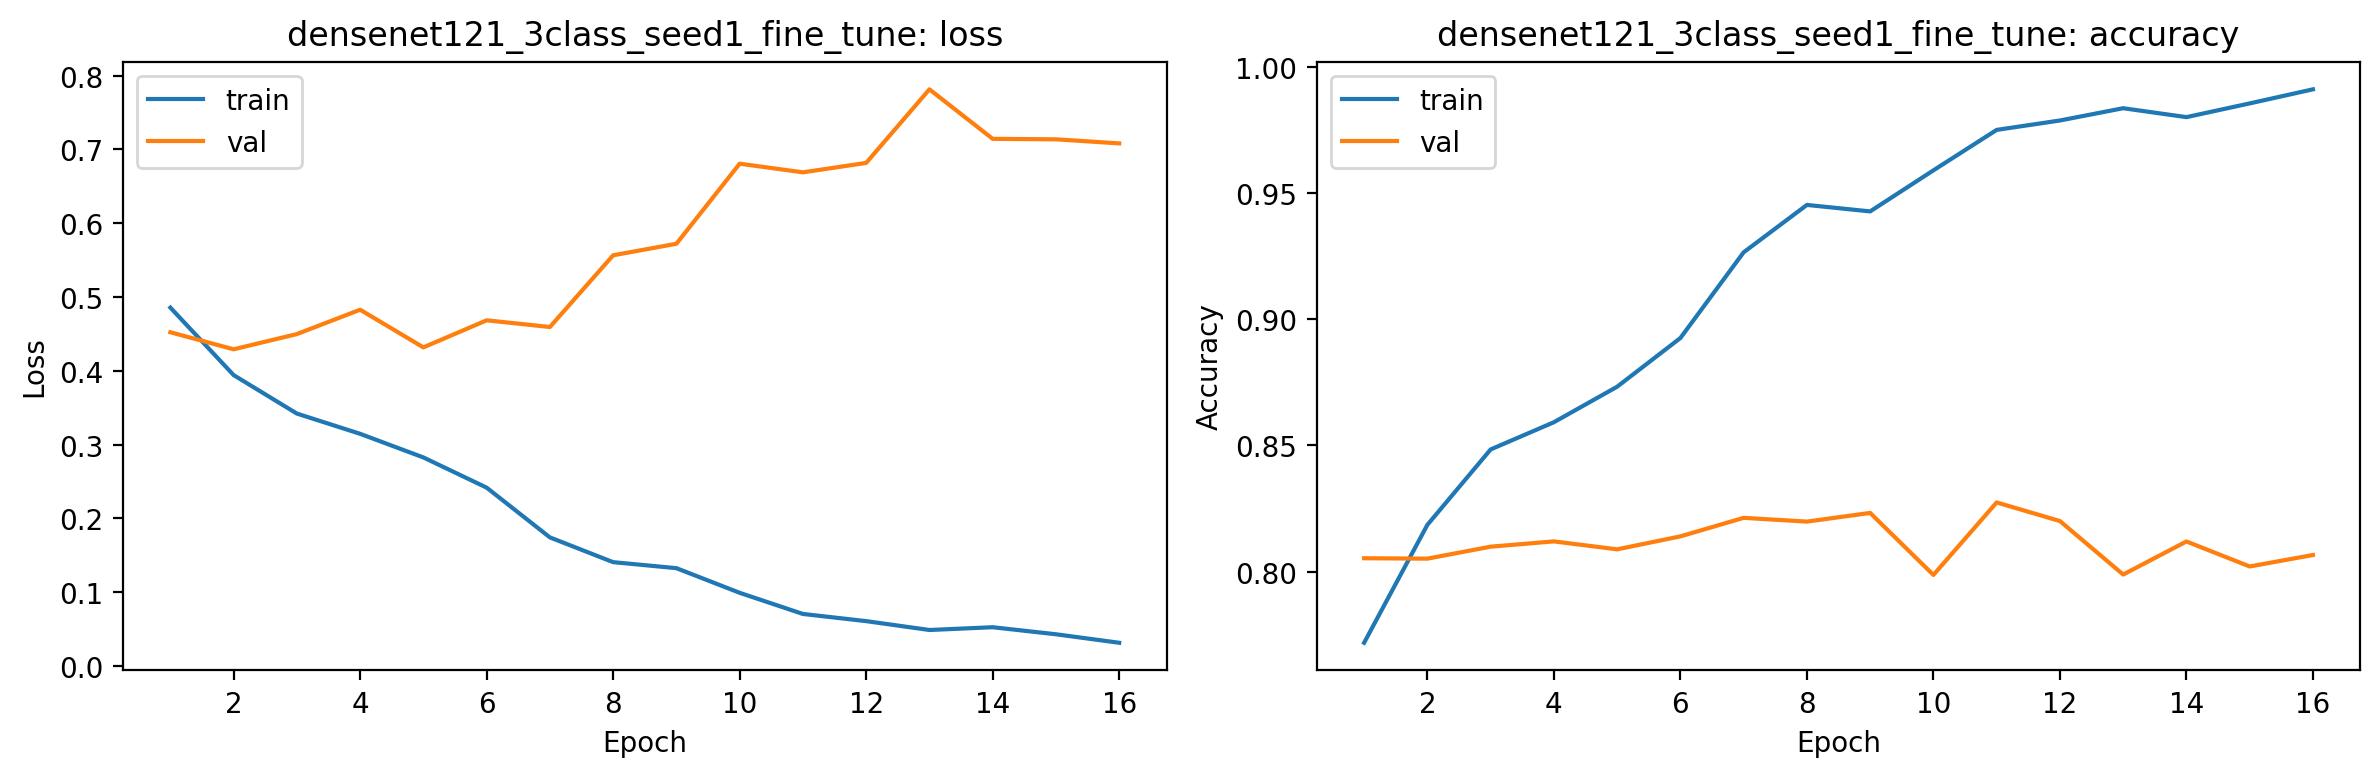
\includegraphics[width=\textwidth]{densenet121_3class_seed1_fine_tune_training_curves.png}
\caption{DenseNet121, seed 1}
\end{subfigure}\\[0.6em]
\begin{subfigure}{0.48\textwidth}
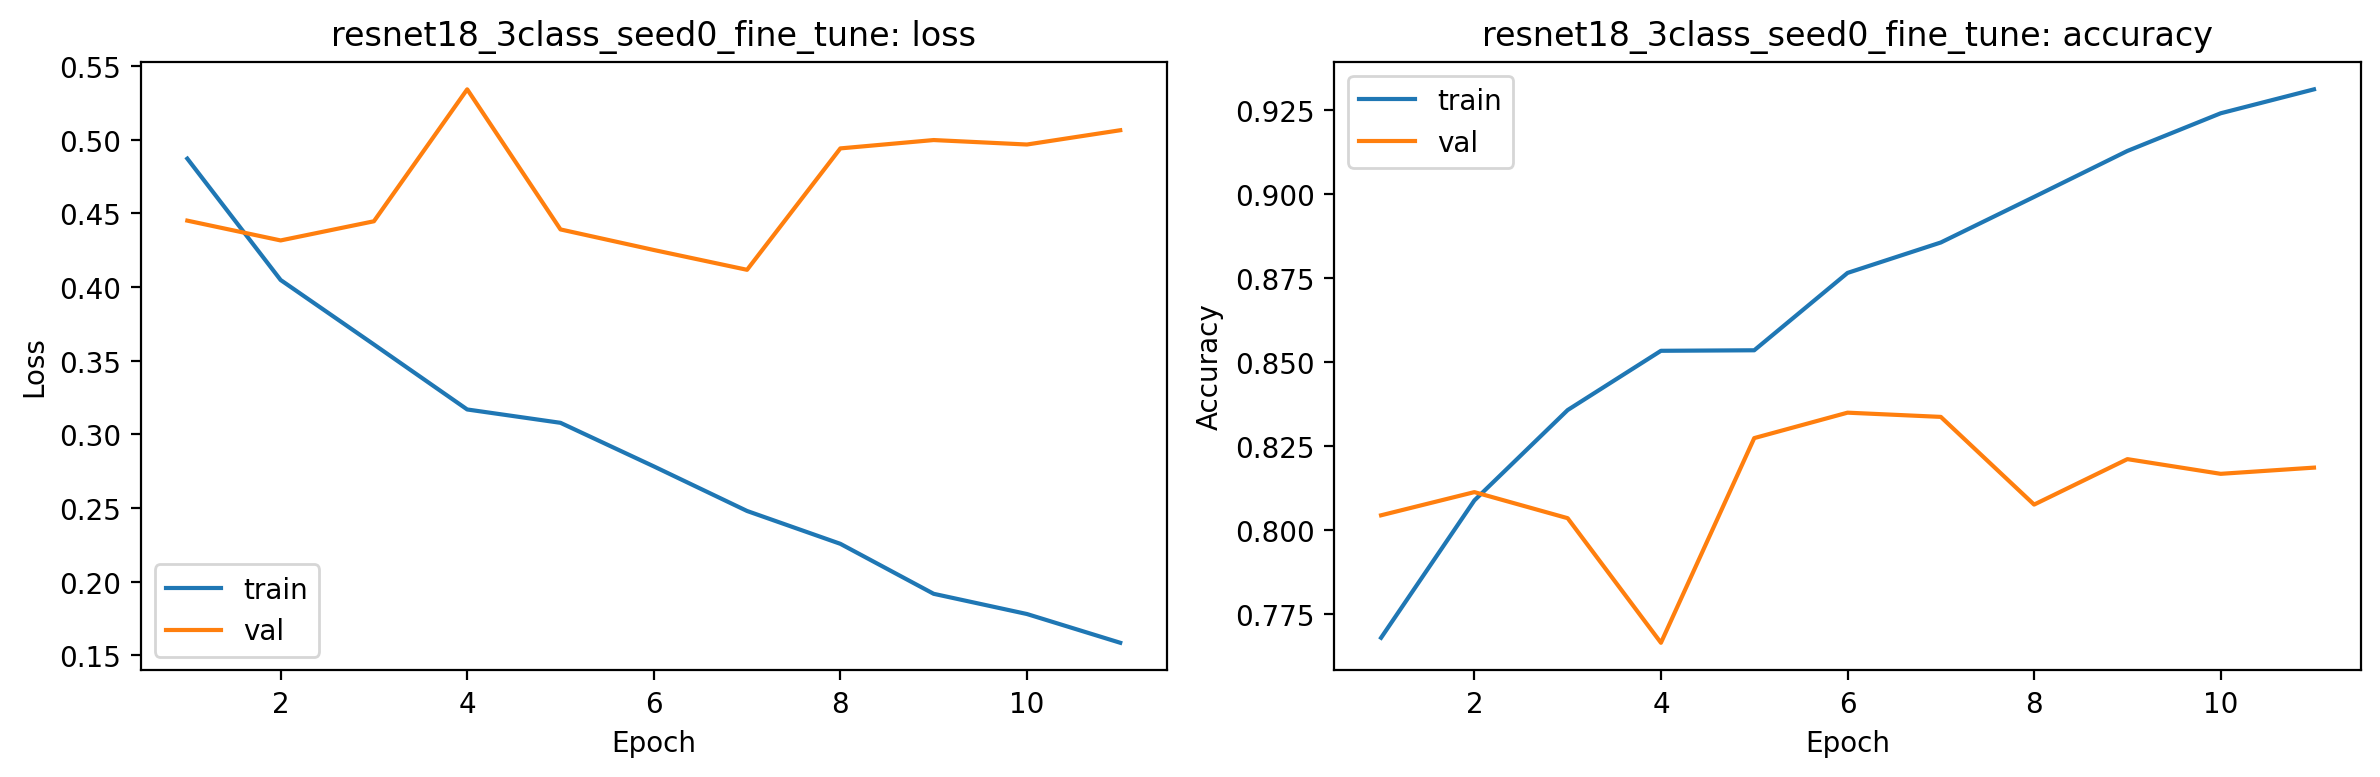
\includegraphics[width=\textwidth]{resnet18_3class_seed0_fine_tune_training_curves.png}
\caption{ResNet18, seed 0}
\end{subfigure}\hfill
\begin{subfigure}{0.48\textwidth}
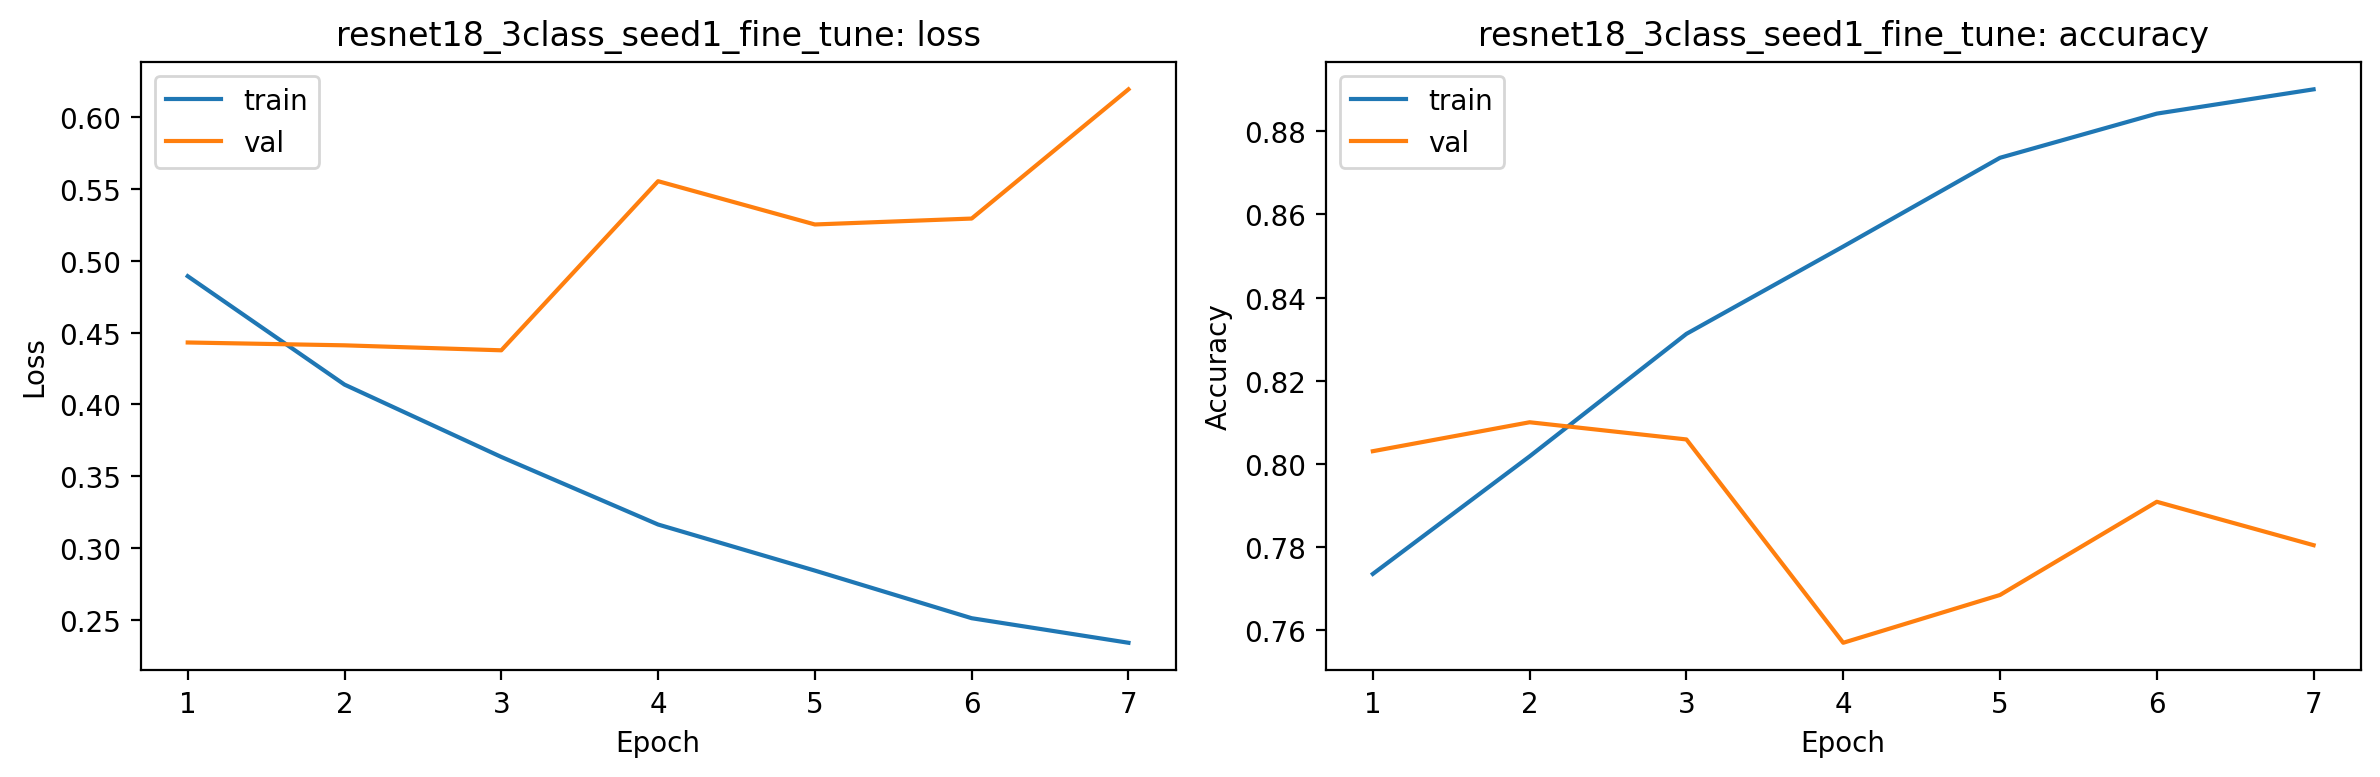
\includegraphics[width=\textwidth]{resnet18_3class_seed1_fine_tune_training_curves.png}
\caption{ResNet18, seed 1}
\end{subfigure}
\caption{Three-class fine-tuning curves (representative seeds) for both
backbones.}
\label{fig:app_curves}
\end{figure}

\FloatBarrier
\subsection{Three-Class Confusion Matrices (per seed)}

Figure~\ref{fig:app_cm} shows the per-seed confusion matrices for
DenseNet121. The NORMAL$\rightarrow$VIRUS confusion is consistent across
seeds, confirming it is a systematic property of the task rather than an
artefact of a single run.

\begin{figure}[h]
\centering
\begin{subfigure}{0.32\textwidth}
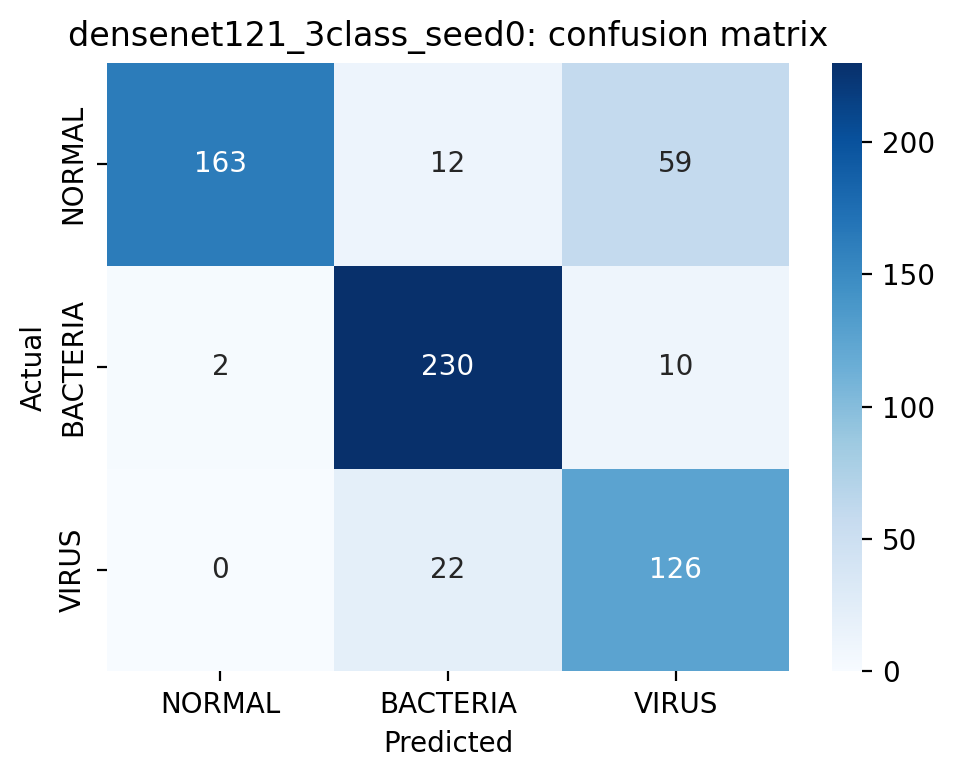
\includegraphics[width=\textwidth]{densenet121_3class_seed0_confusion_matrix.png}
\caption{seed 0}
\end{subfigure}\hfill
\begin{subfigure}{0.32\textwidth}
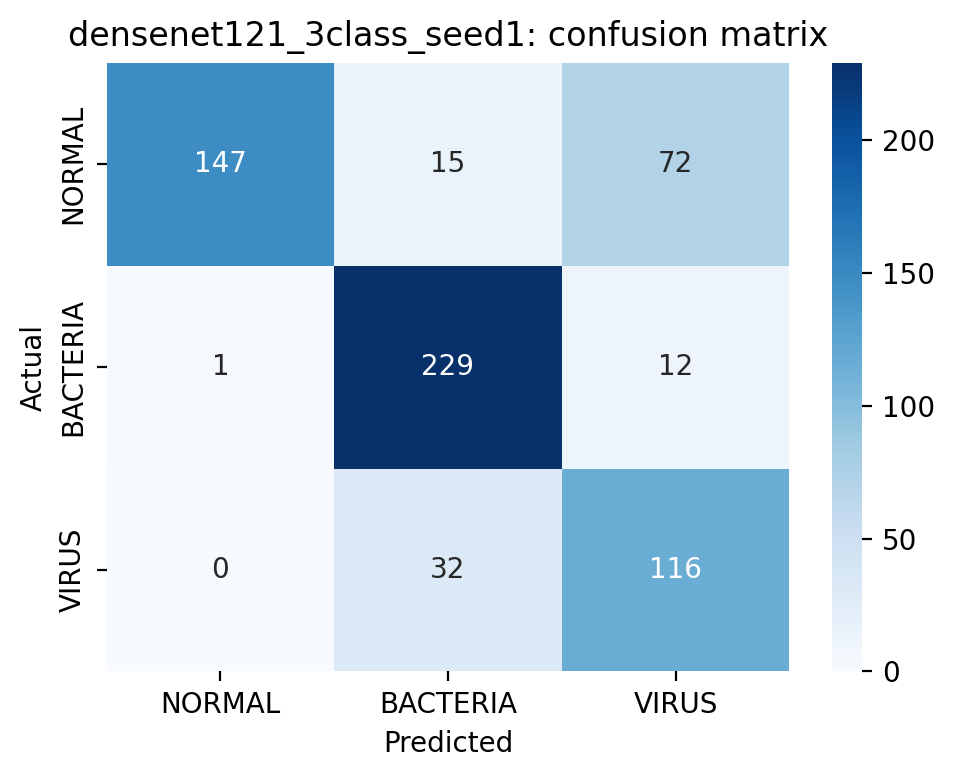
\includegraphics[width=\textwidth]{densenet121_3class_seed1_confusion_matrix.png}
\caption{seed 1}
\end{subfigure}\hfill
\begin{subfigure}{0.32\textwidth}
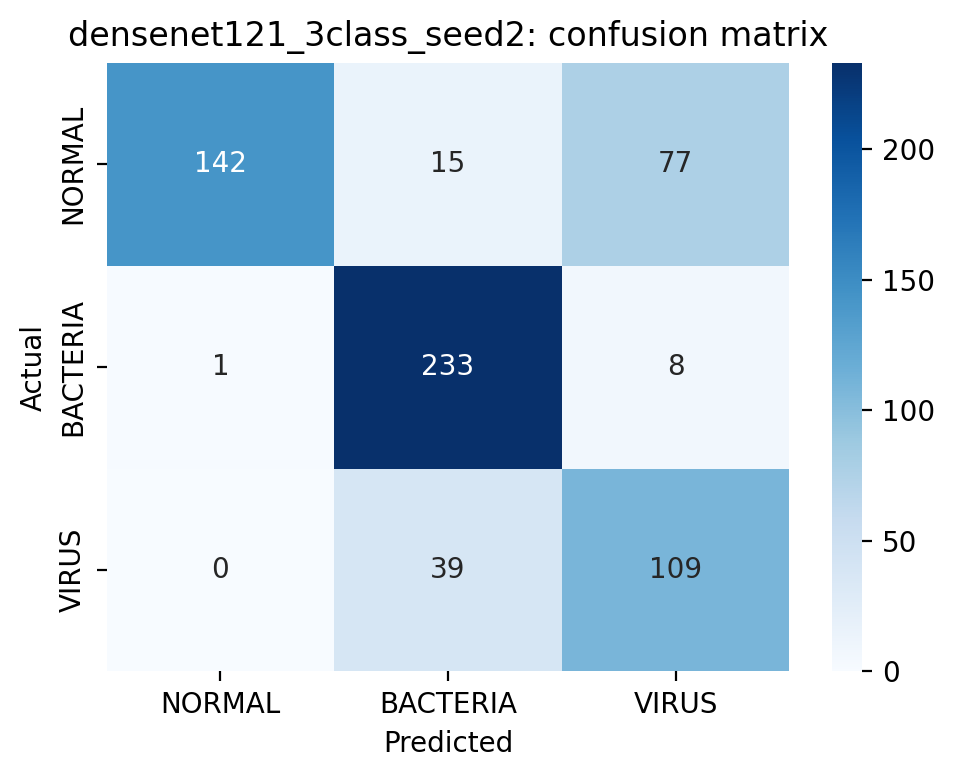
\includegraphics[width=\textwidth]{densenet121_3class_seed2_confusion_matrix.png}
\caption{seed 2}
\end{subfigure}
\caption{Per-seed three-class confusion matrices for DenseNet121.}
\label{fig:app_cm}
\end{figure}

\FloatBarrier
\subsection{Additional Grad-CAM Examples}

Figure~\ref{fig:app_gradcam} provides further three-class Grad-CAM examples,
including additional failure modes (BACTERIA misread as VIRUS, and NORMAL
misread as BACTERIA).

\begin{figure}[H]
\centering
\begin{subfigure}{0.24\textwidth}
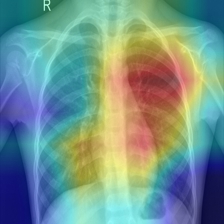
\includegraphics[width=\textwidth]{densenet121_3class_correct_NORMAL_IM-0001-0001.png}
\caption{Correct: NORMAL}
\end{subfigure}\hfill
\begin{subfigure}{0.24\textwidth}
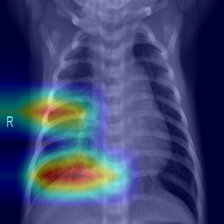
\includegraphics[width=\textwidth]{densenet121_3class_wrong_BACTERIA_as_VIRUS_person117_bacteria_5.png}
\caption{Error: BACTERIA as VIRUS}
\end{subfigure}\hfill
\begin{subfigure}{0.24\textwidth}
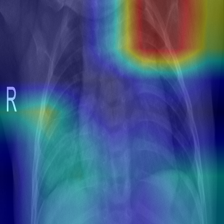
\includegraphics[width=\textwidth]{densenet121_3class_wrong_NORMAL_as_BACTERIA_IM-0022-0001.png}
\caption{Error: NORMAL as BACTERIA}
\end{subfigure}
\caption{Additional three-class Grad-CAM overlays (DenseNet121).}
\label{fig:app_gradcam}
\end{figure}

\subsection{Complete Figure Set}

For completeness, this subsection collects every remaining figure produced by the pipeline that is not shown in the main text or above: all per-seed confusion matrices and training curves for both tasks, the per-seed Grad-CAM overlays for ResNet18, and a few task-level summary figures. They are included for reproducibility and add no new claims.

\begin{figure}[H]
\centering
\begin{subfigure}{0.22\textwidth}
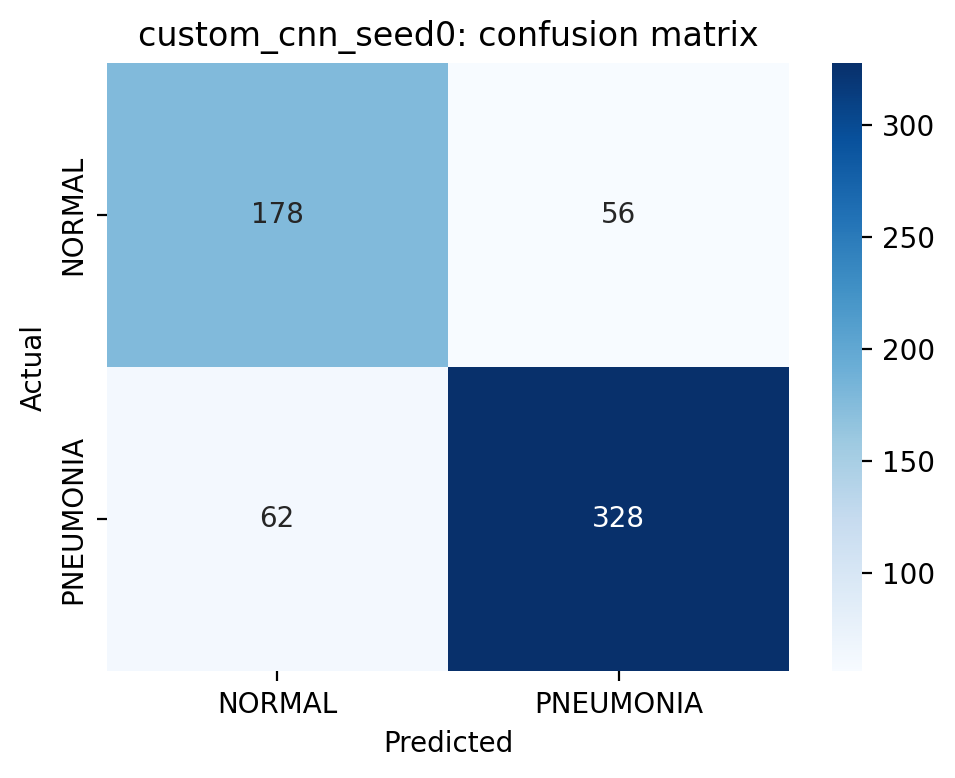
\includegraphics[width=\textwidth]{custom_cnn_seed0_confusion_matrix.png}
\caption{custom cnn seed0}
\end{subfigure}\hfill
\begin{subfigure}{0.22\textwidth}
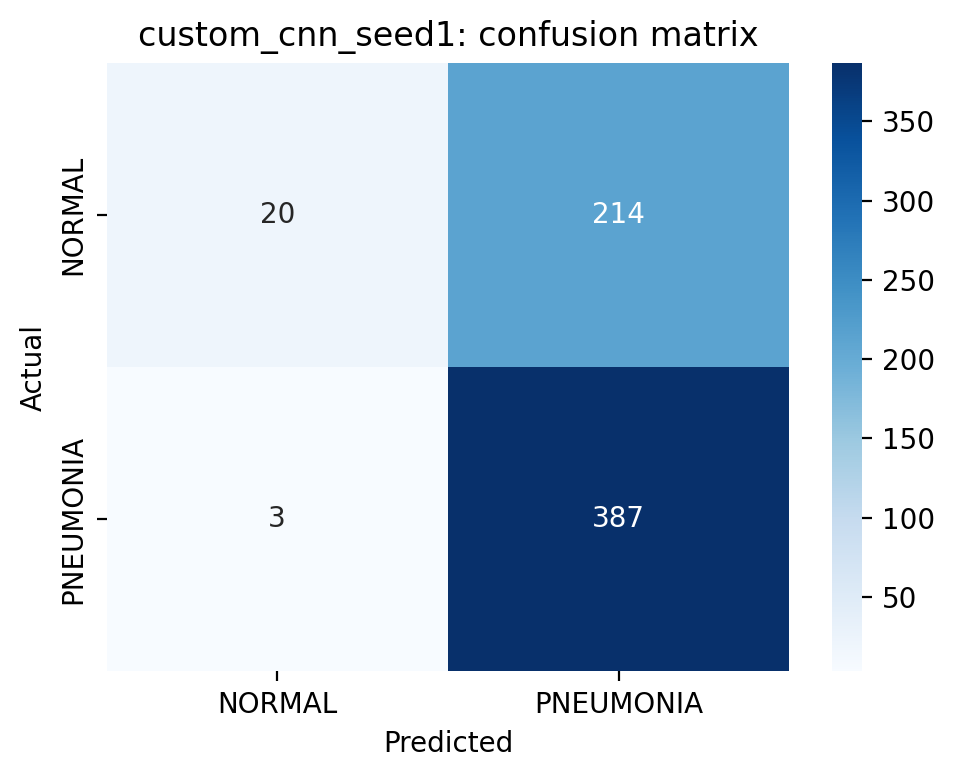
\includegraphics[width=\textwidth]{custom_cnn_seed1_confusion_matrix.png}
\caption{custom cnn seed1}
\end{subfigure}\hfill
\begin{subfigure}{0.22\textwidth}
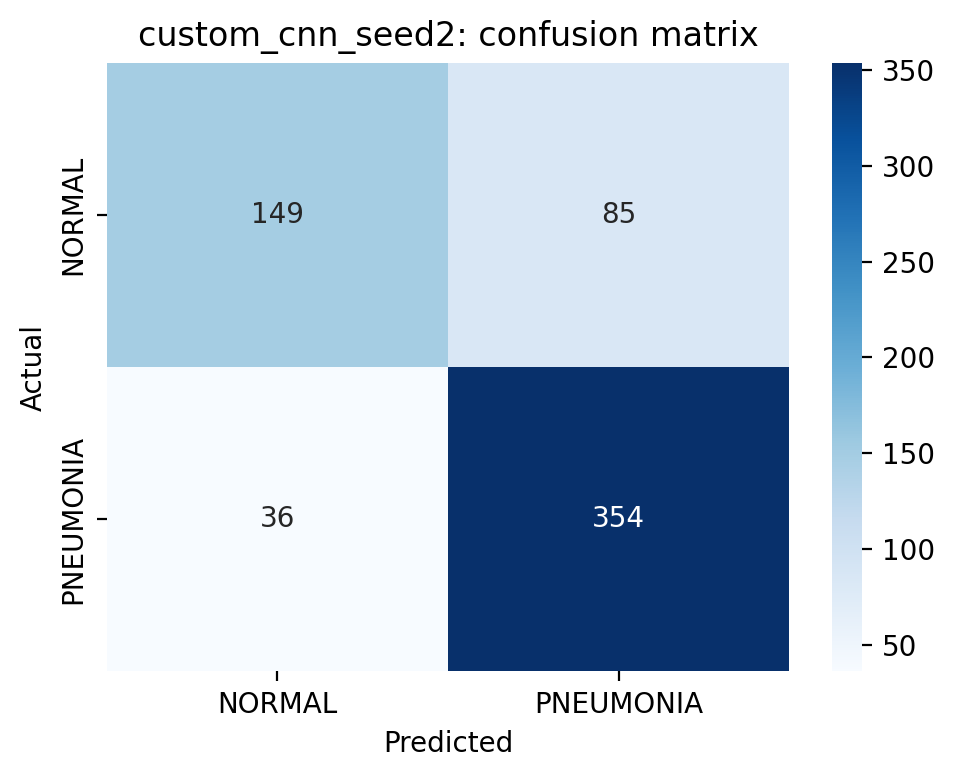
\includegraphics[width=\textwidth]{custom_cnn_seed2_confusion_matrix.png}
\caption{custom cnn seed2}
\end{subfigure}\\[0.3em]
\begin{subfigure}{0.22\textwidth}
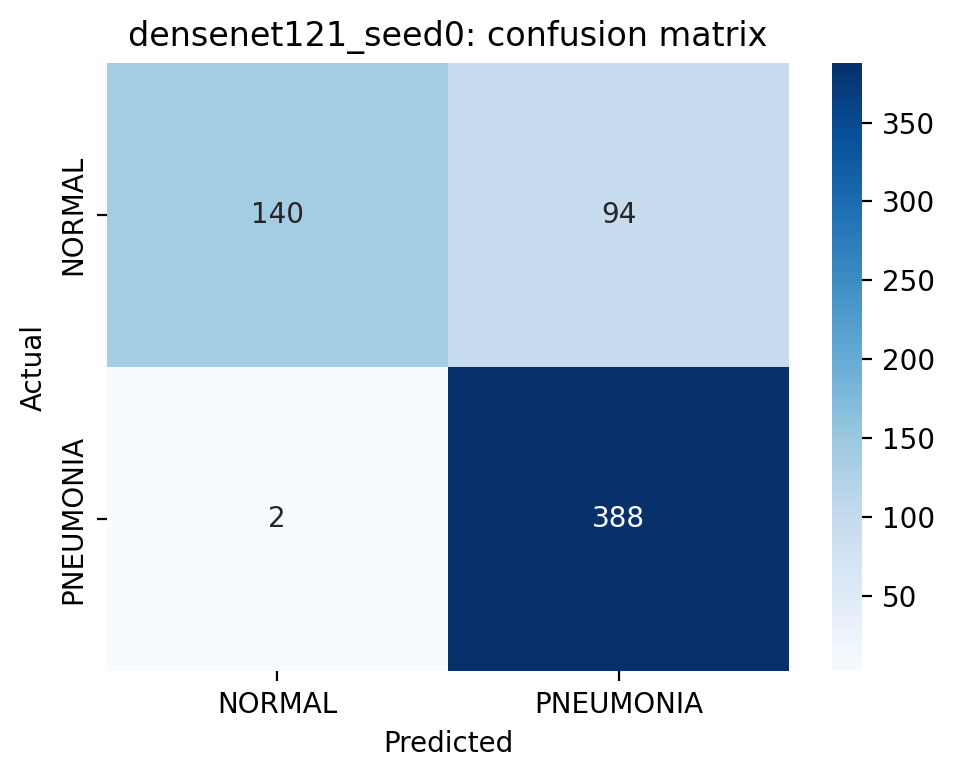
\includegraphics[width=\textwidth]{densenet121_seed0_confusion_matrix.png}
\caption{densenet121 seed0}
\end{subfigure}\hfill
\begin{subfigure}{0.22\textwidth}
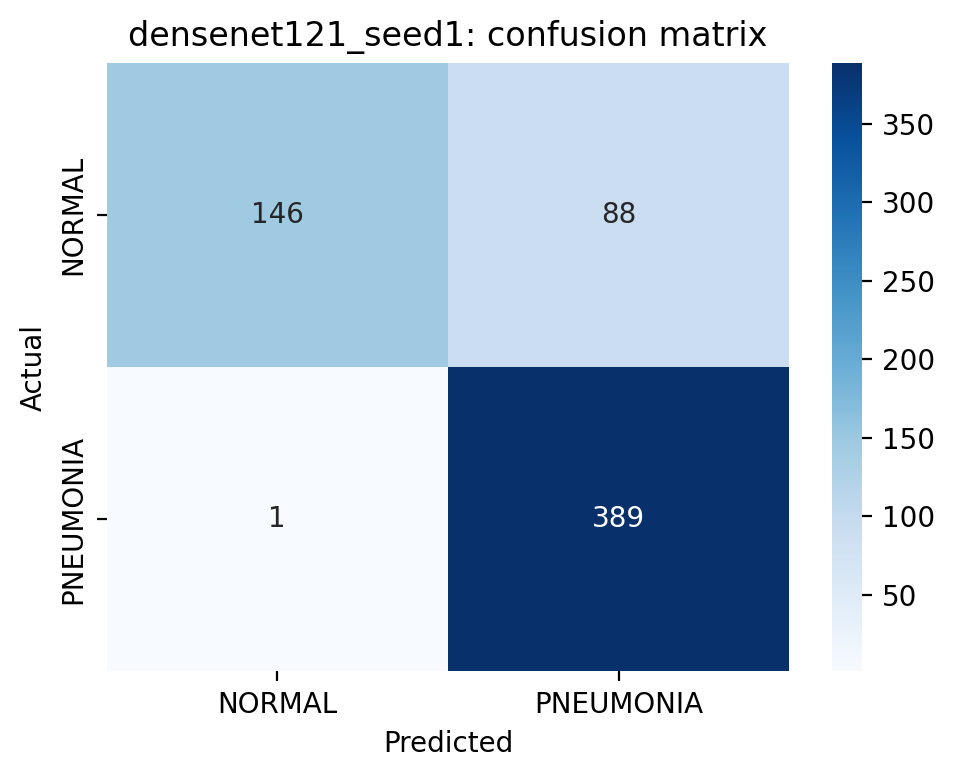
\includegraphics[width=\textwidth]{densenet121_seed1_confusion_matrix.png}
\caption{densenet121 seed1}
\end{subfigure}\hfill
\begin{subfigure}{0.22\textwidth}
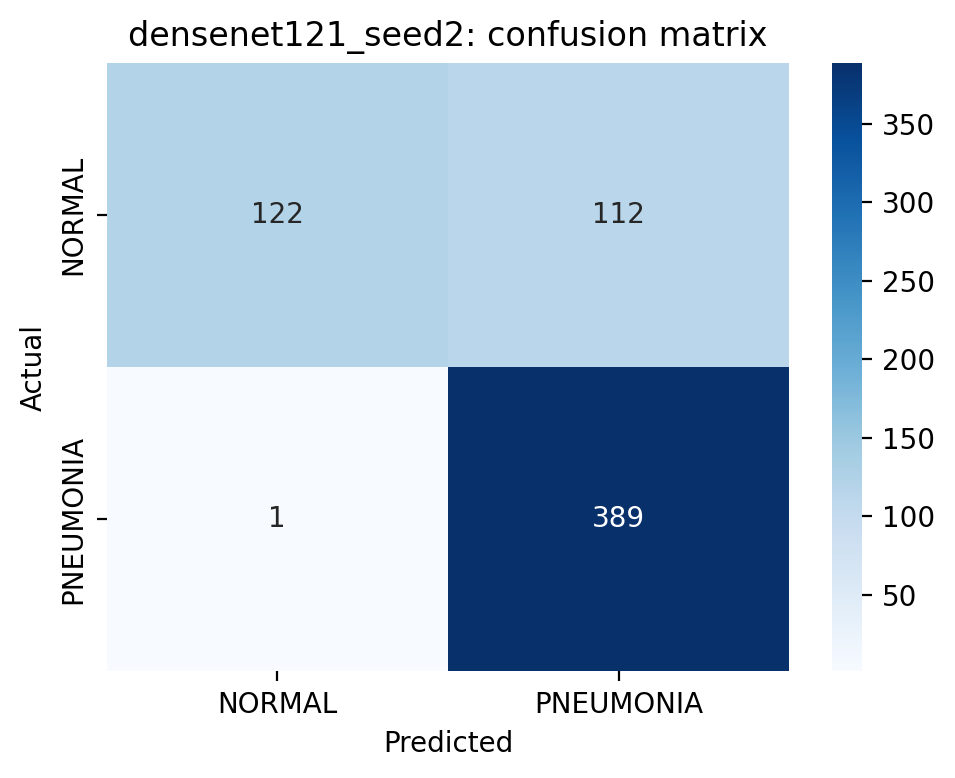
\includegraphics[width=\textwidth]{densenet121_seed2_confusion_matrix.png}
\caption{densenet121 seed2}
\end{subfigure}\\[0.3em]
\begin{subfigure}{0.22\textwidth}
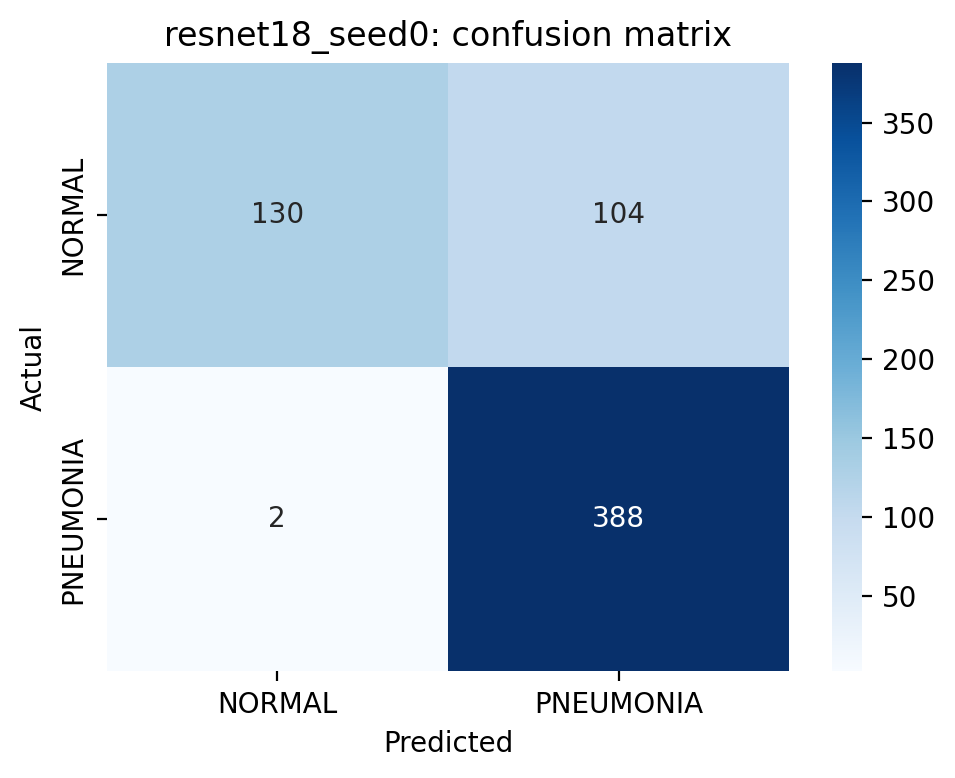
\includegraphics[width=\textwidth]{resnet18_seed0_confusion_matrix.png}
\caption{resnet18 seed0}
\end{subfigure}\hfill
\begin{subfigure}{0.22\textwidth}
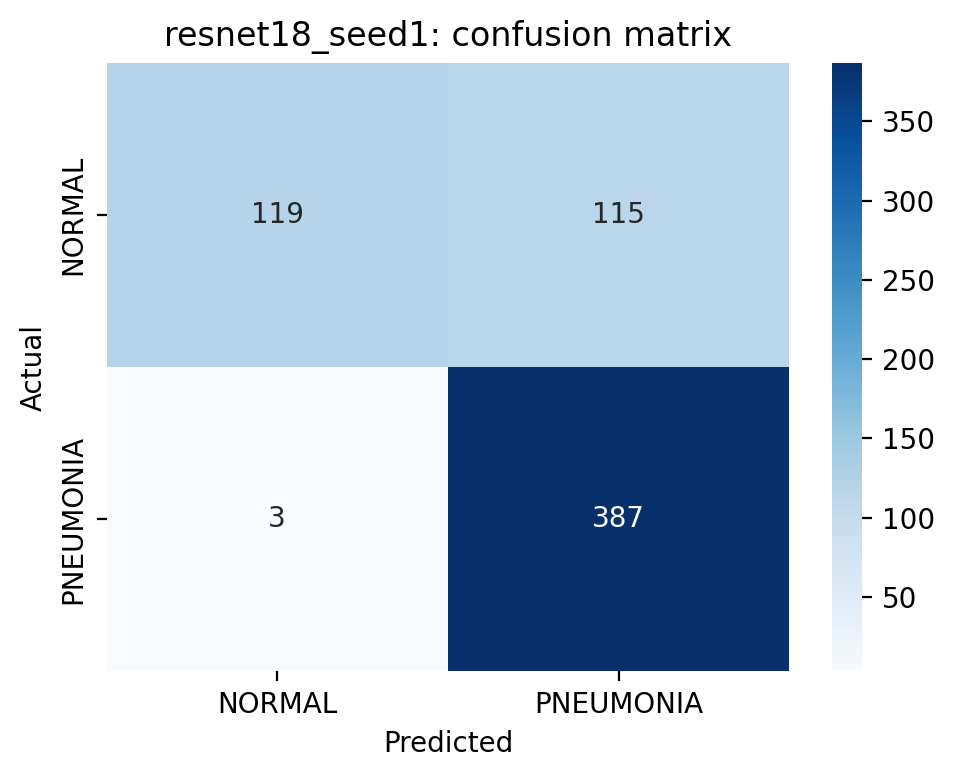
\includegraphics[width=\textwidth]{resnet18_seed1_confusion_matrix.png}
\caption{resnet18 seed1}
\end{subfigure}\hfill
\begin{subfigure}{0.22\textwidth}
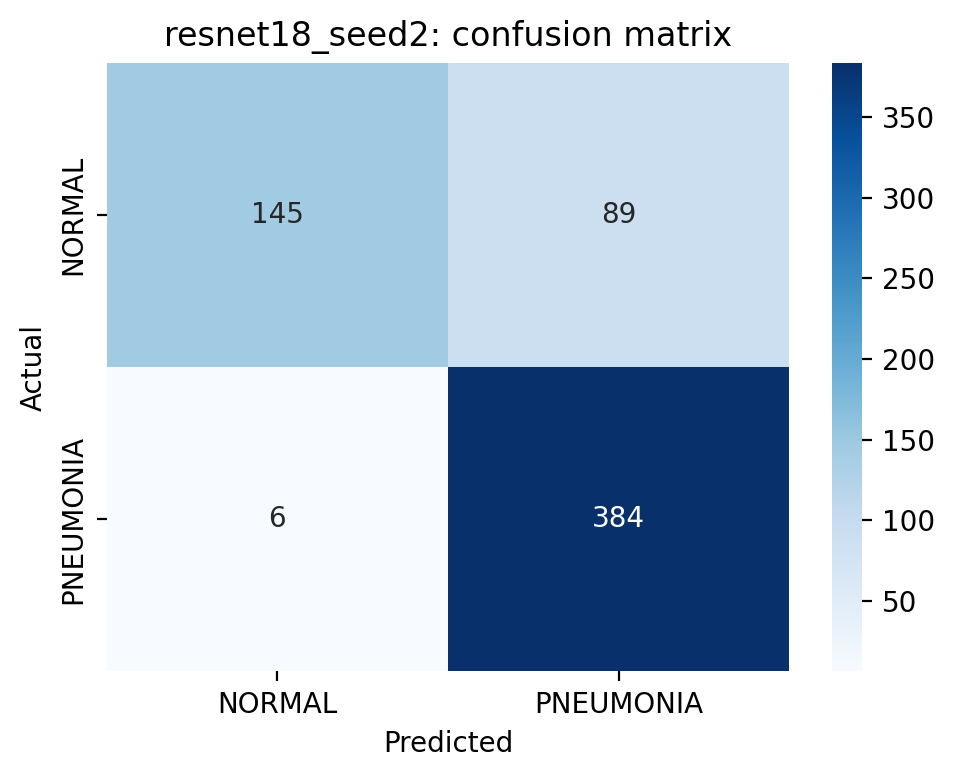
\includegraphics[width=\textwidth]{resnet18_seed2_confusion_matrix.png}
\caption{resnet18 seed2}
\end{subfigure}
\caption{Binary confusion matrices (per seed), all models.}
\label{fig:app_cmb}
\end{figure}
\FloatBarrier

\begin{figure}[h]
\centering
\begin{subfigure}{0.45\textwidth}
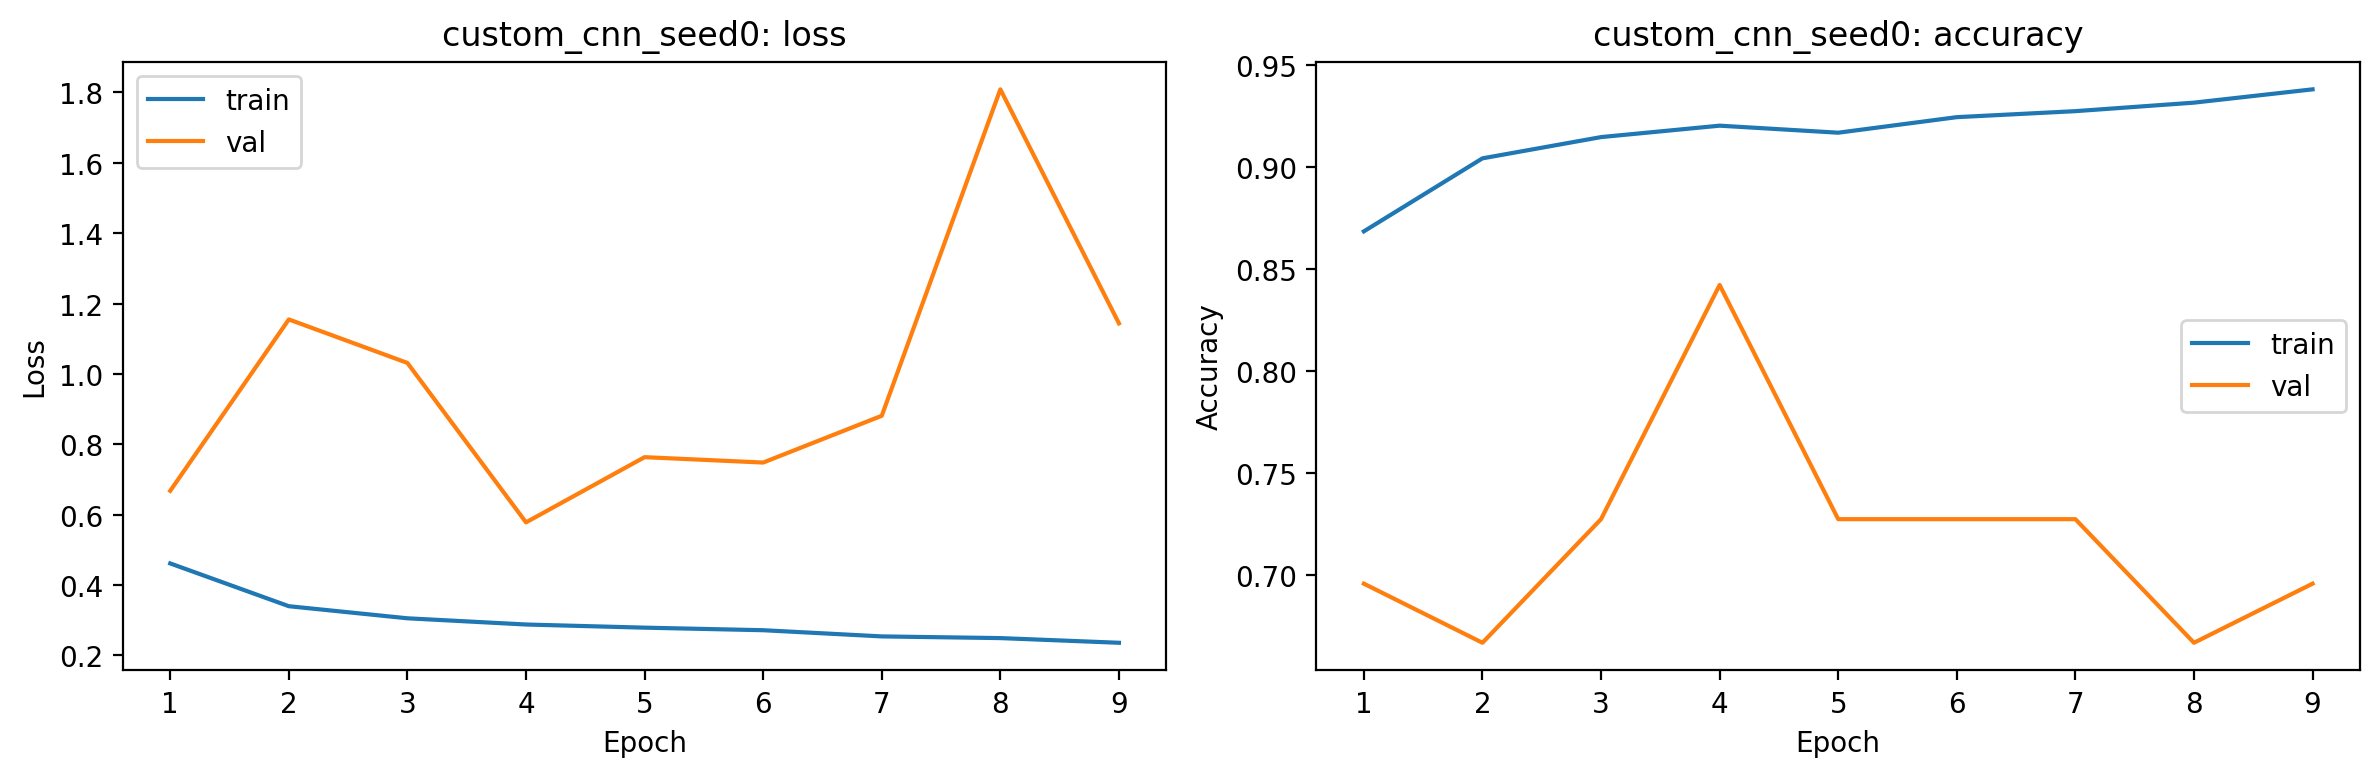
\includegraphics[width=\textwidth]{custom_cnn_seed0_training_curves.png}
\caption{custom cnn seed0 training curves}
\end{subfigure}\hfill
\begin{subfigure}{0.45\textwidth}
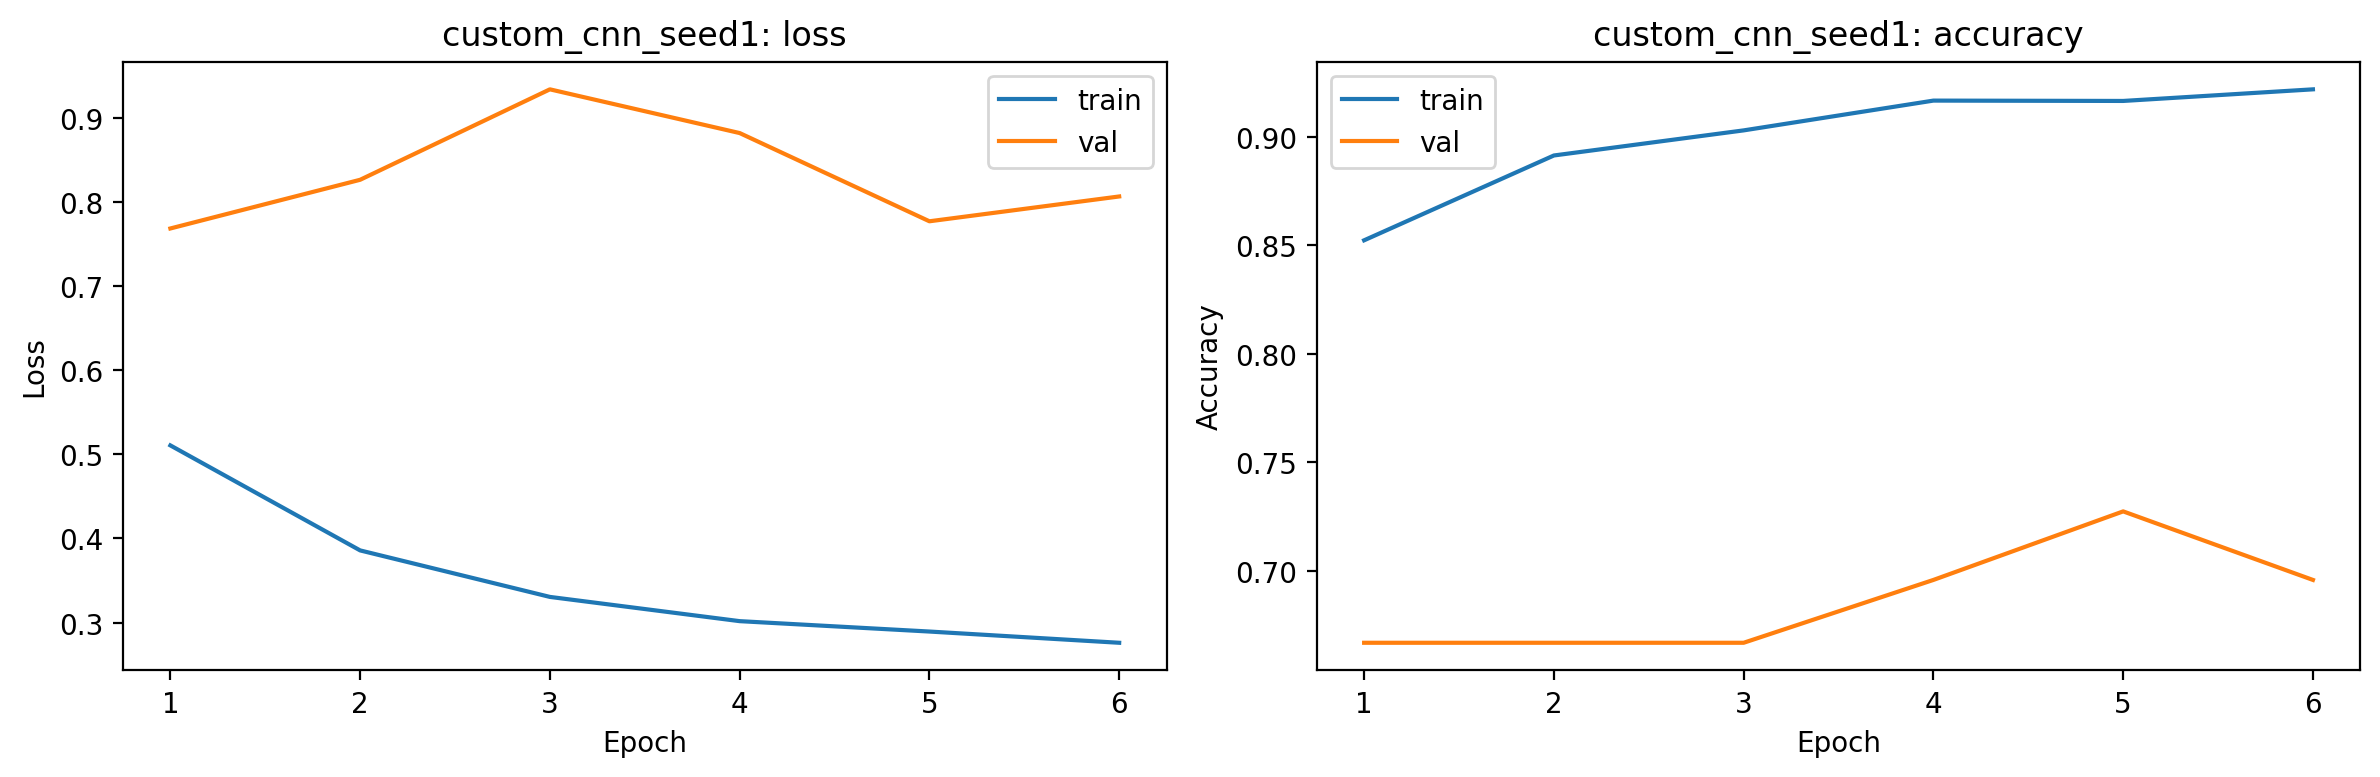
\includegraphics[width=\textwidth]{custom_cnn_seed1_training_curves.png}
\caption{custom cnn seed1 training curves}
\end{subfigure}\\[0.6em]
\begin{subfigure}{0.45\textwidth}
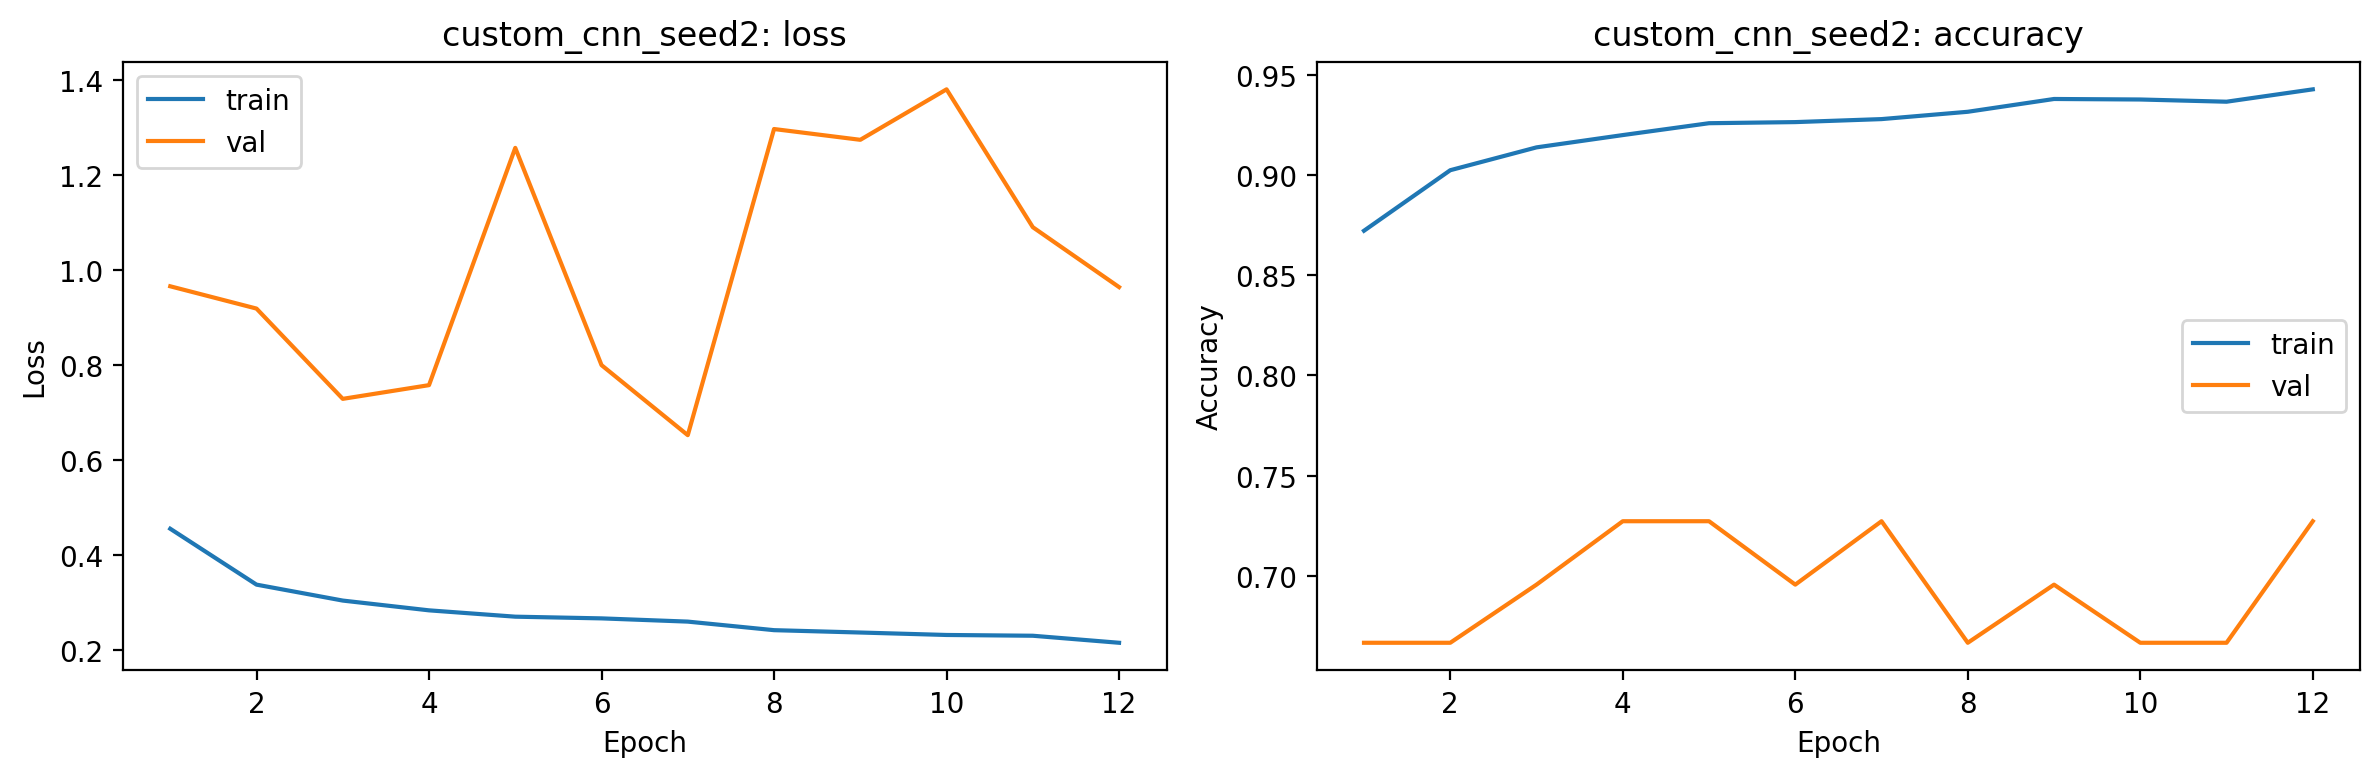
\includegraphics[width=\textwidth]{custom_cnn_seed2_training_curves.png}
\caption{custom cnn seed2 training curves}
\end{subfigure}\hfill
\begin{subfigure}{0.45\textwidth}
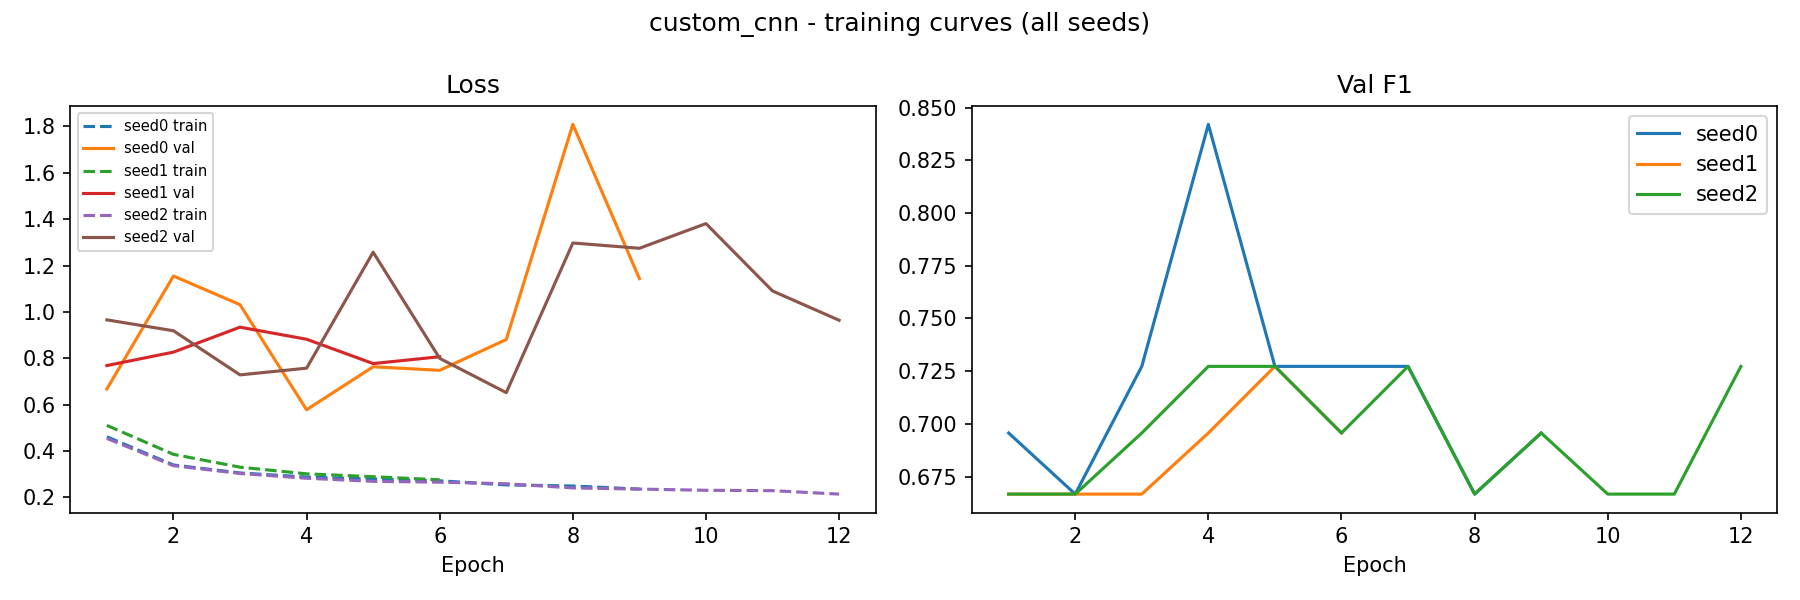
\includegraphics[width=\textwidth]{custom_cnn_training_curves.png}
\caption{custom cnn training curves}
\end{subfigure}\\[0.6em]
\begin{subfigure}{0.45\textwidth}
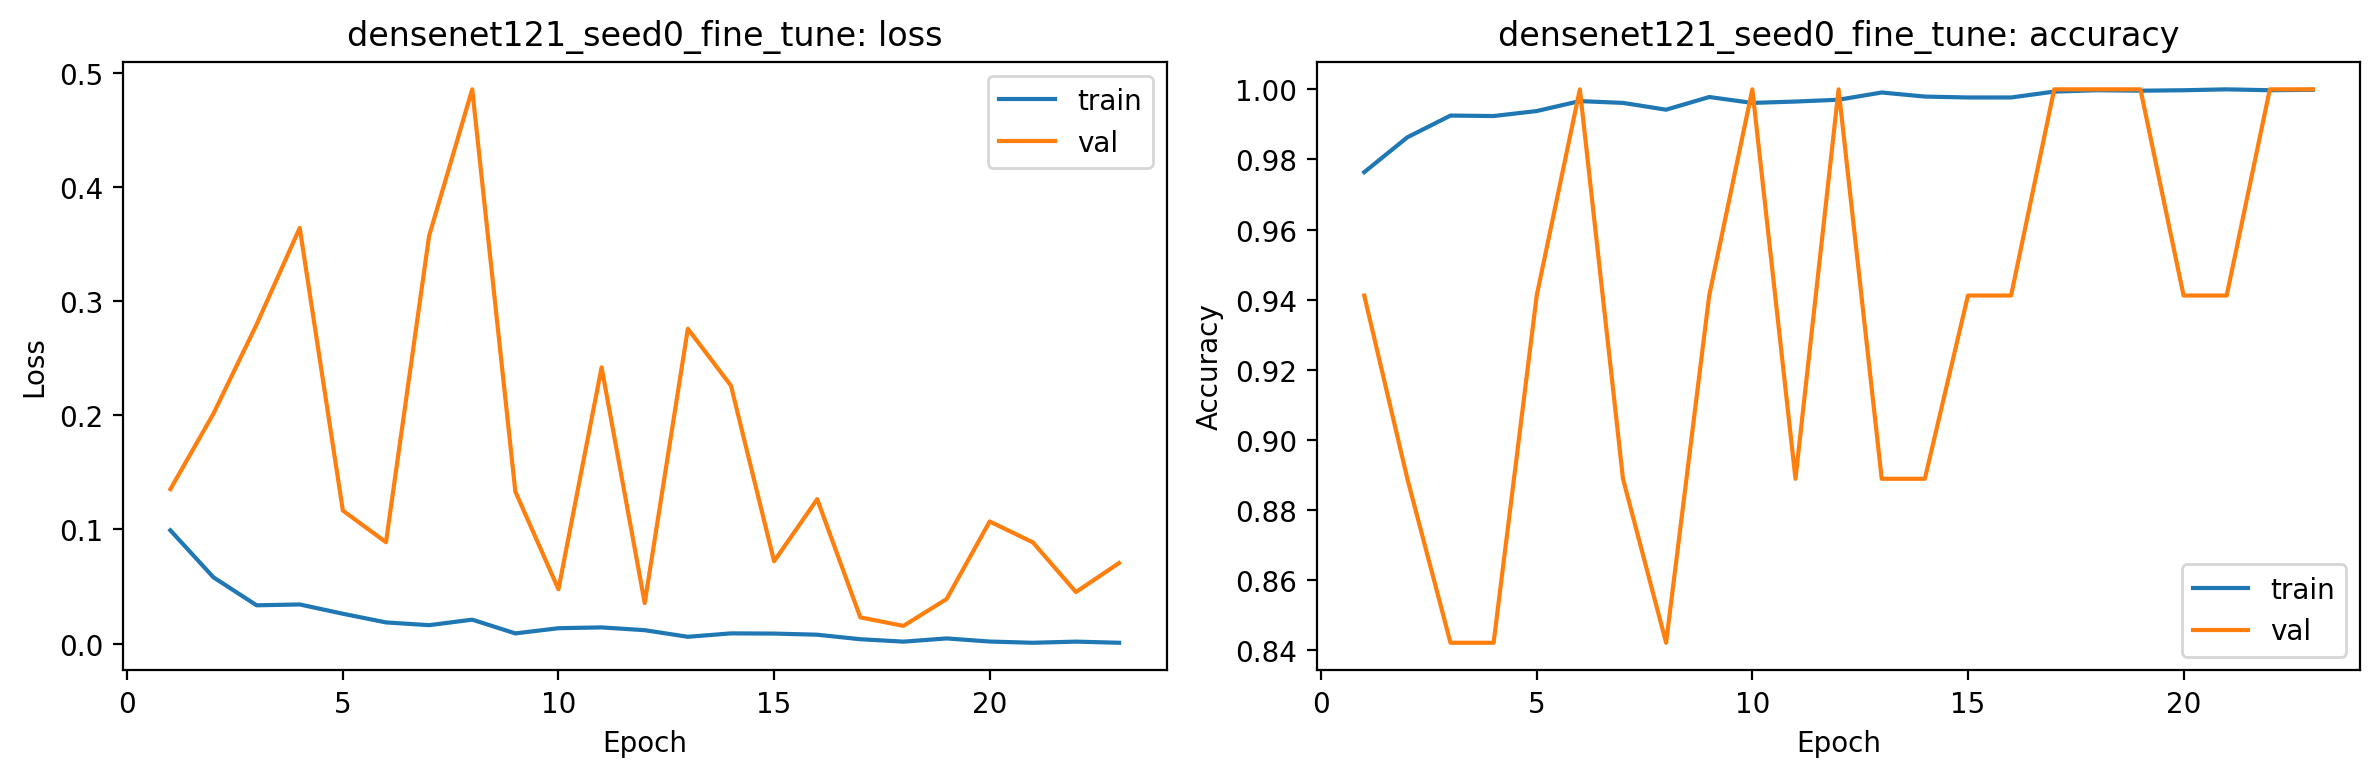
\includegraphics[width=\textwidth]{densenet121_seed0_fine_tune_training_curves.png}
\caption{densenet121 seed0 fine tune training curves}
\end{subfigure}\hfill
\begin{subfigure}{0.45\textwidth}
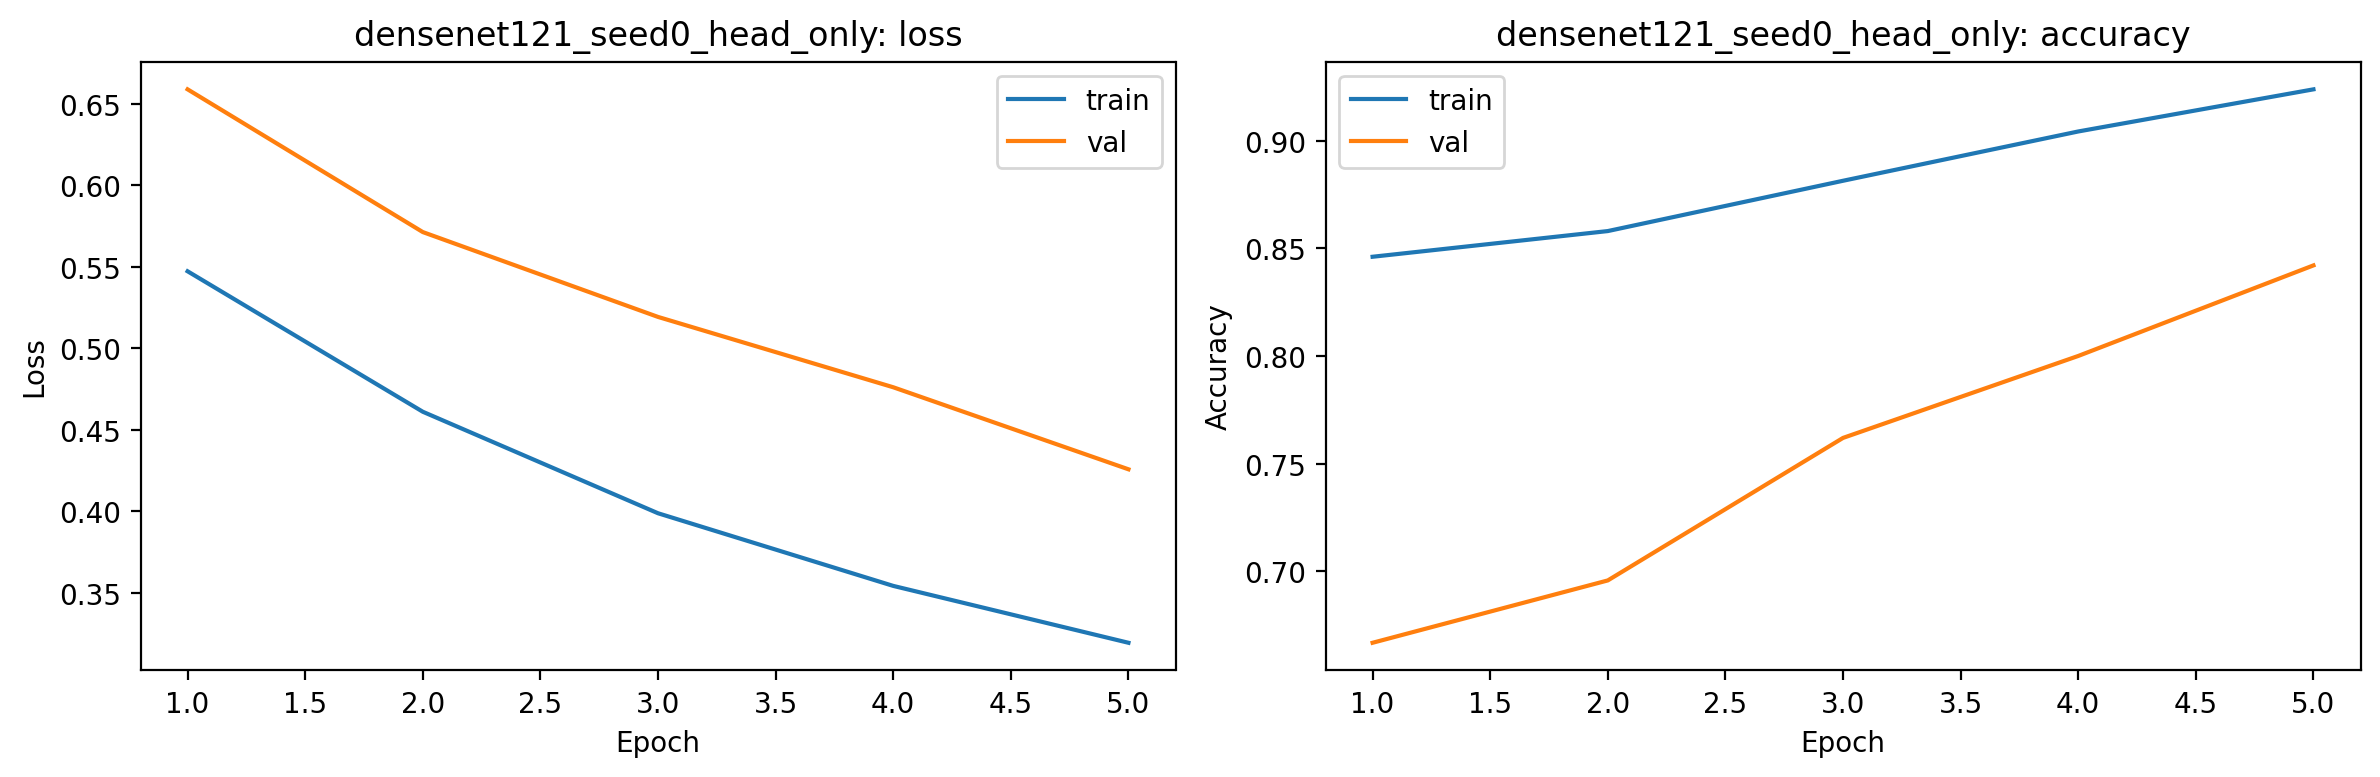
\includegraphics[width=\textwidth]{densenet121_seed0_head_only_training_curves.png}
\caption{densenet121 seed0 head only training curves}
\end{subfigure}\\[0.6em]
\begin{subfigure}{0.45\textwidth}
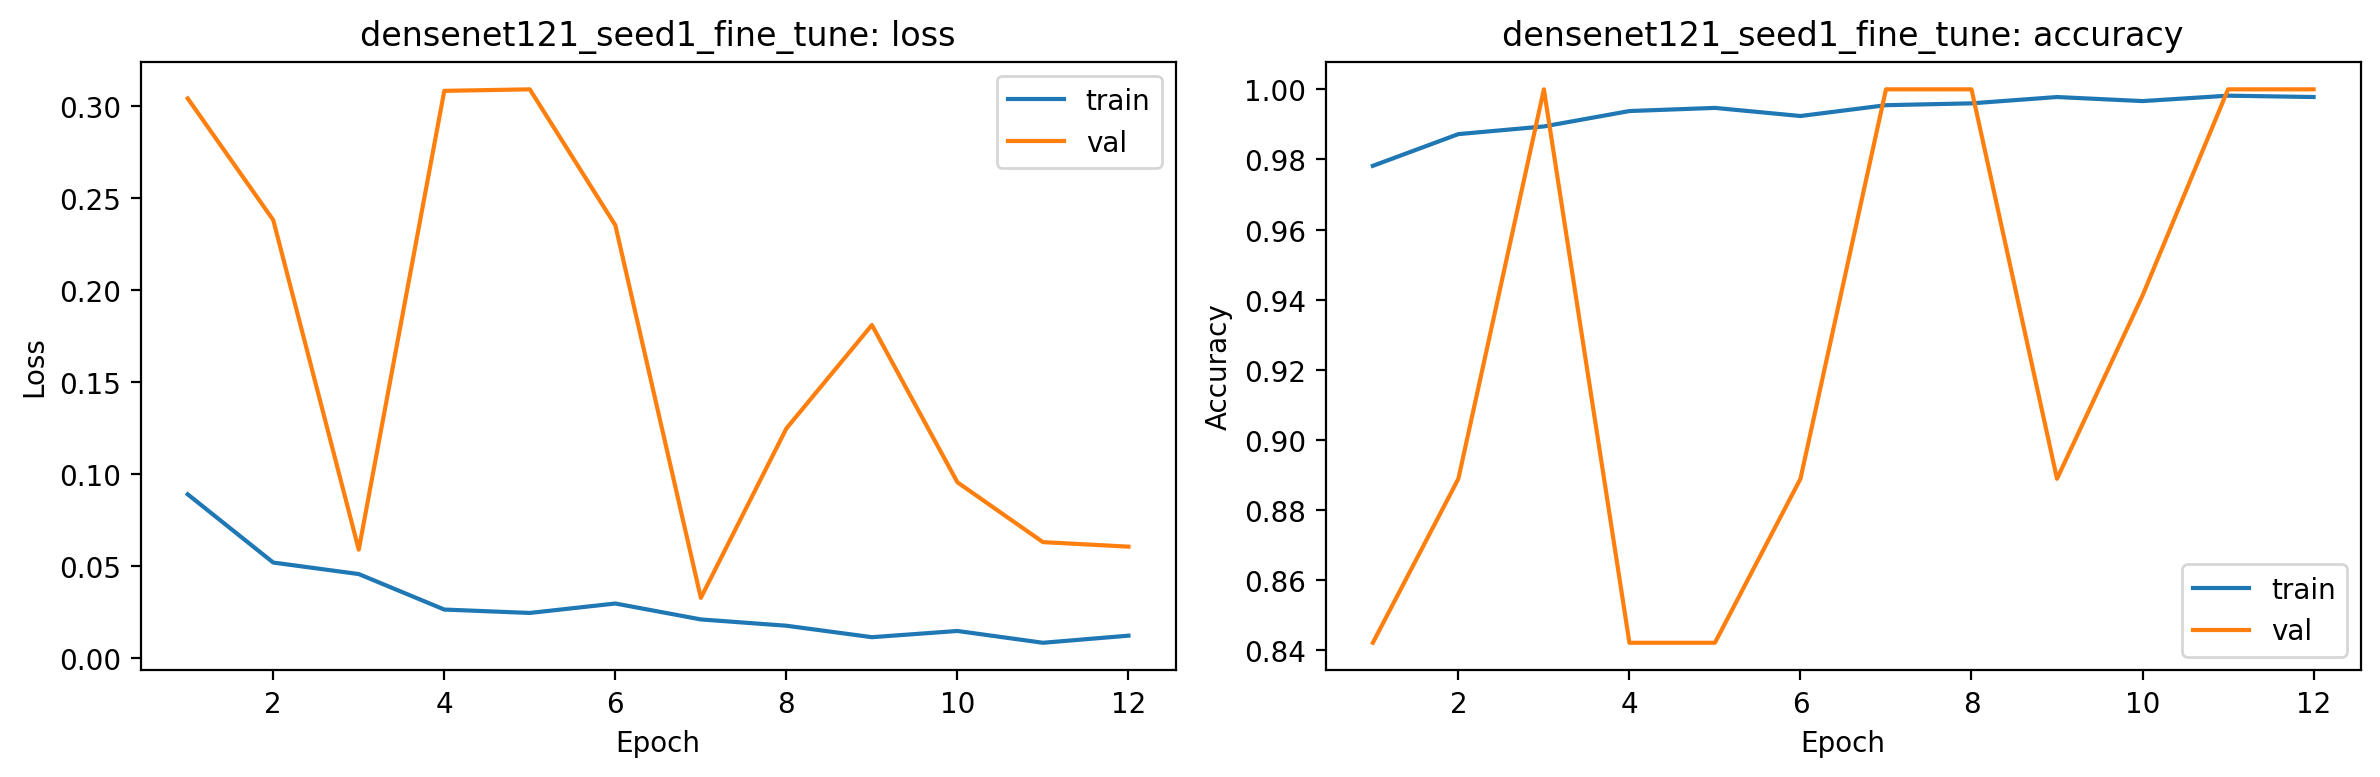
\includegraphics[width=\textwidth]{densenet121_seed1_fine_tune_training_curves.png}
\caption{densenet121 seed1 fine tune training curves}
\end{subfigure}\hfill
\begin{subfigure}{0.45\textwidth}
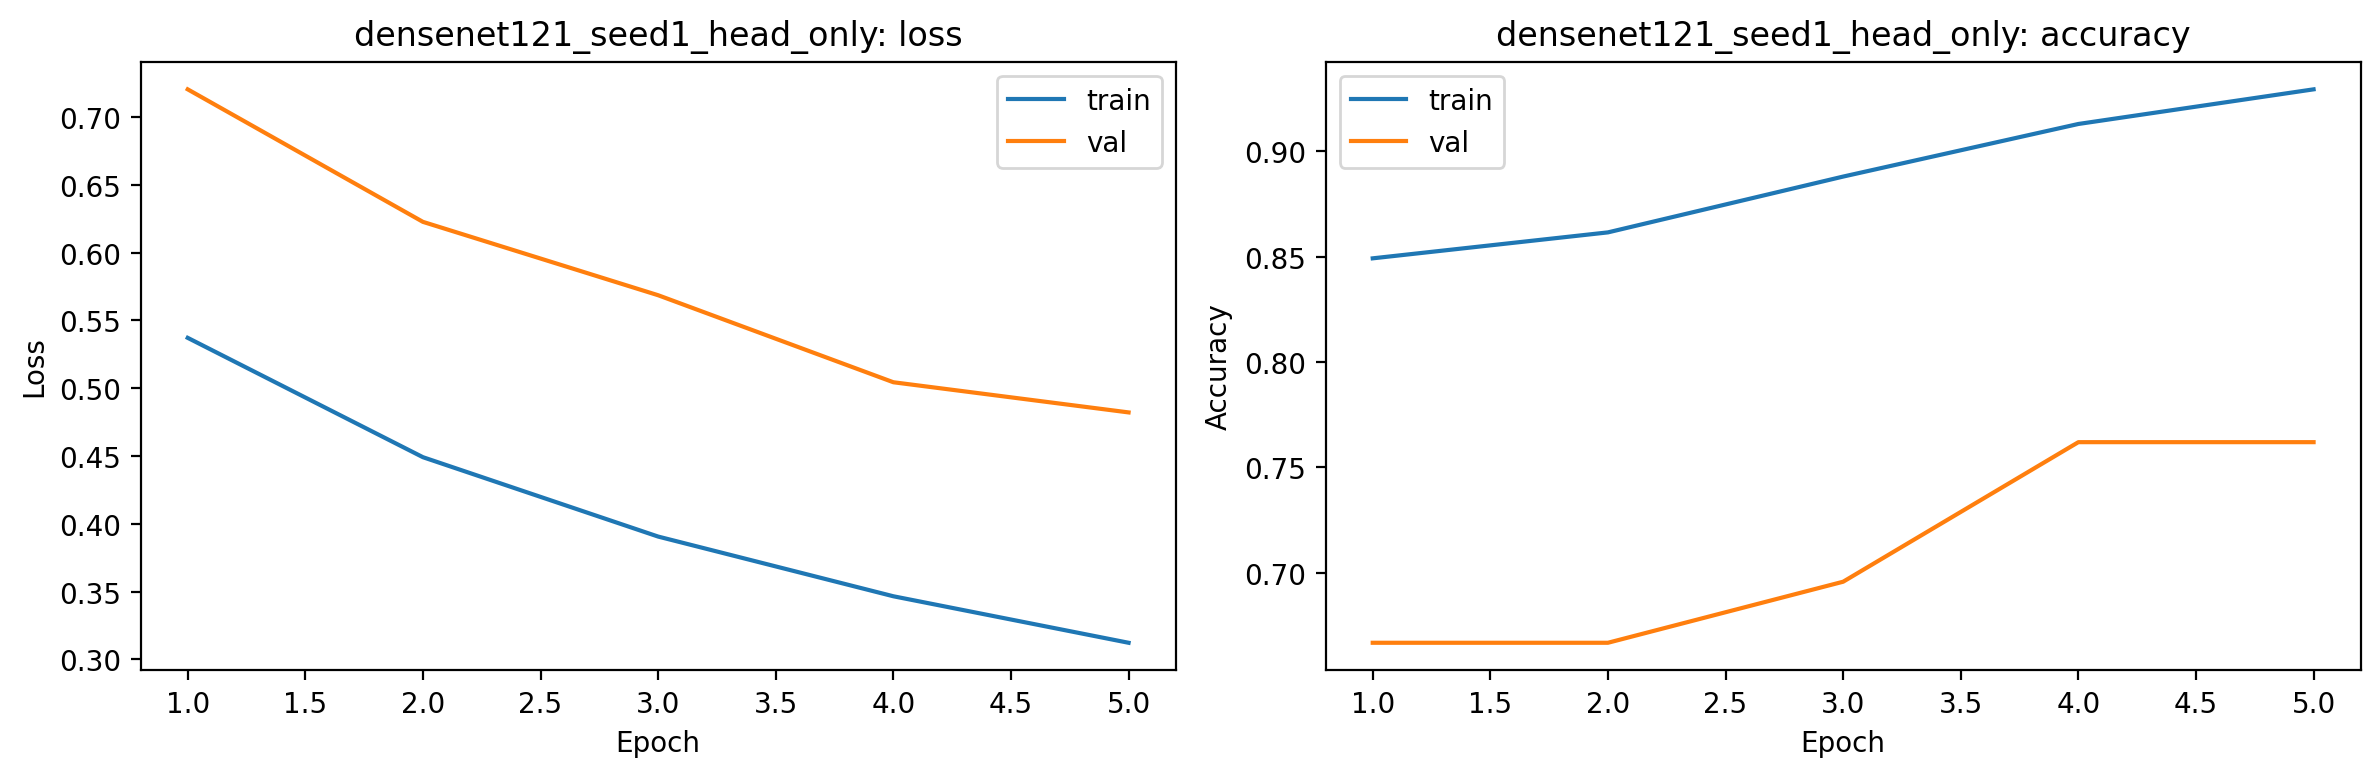
\includegraphics[width=\textwidth]{densenet121_seed1_head_only_training_curves.png}
\caption{densenet121 seed1 head only training curves}
\end{subfigure}\\[0.6em]
\begin{subfigure}{0.45\textwidth}
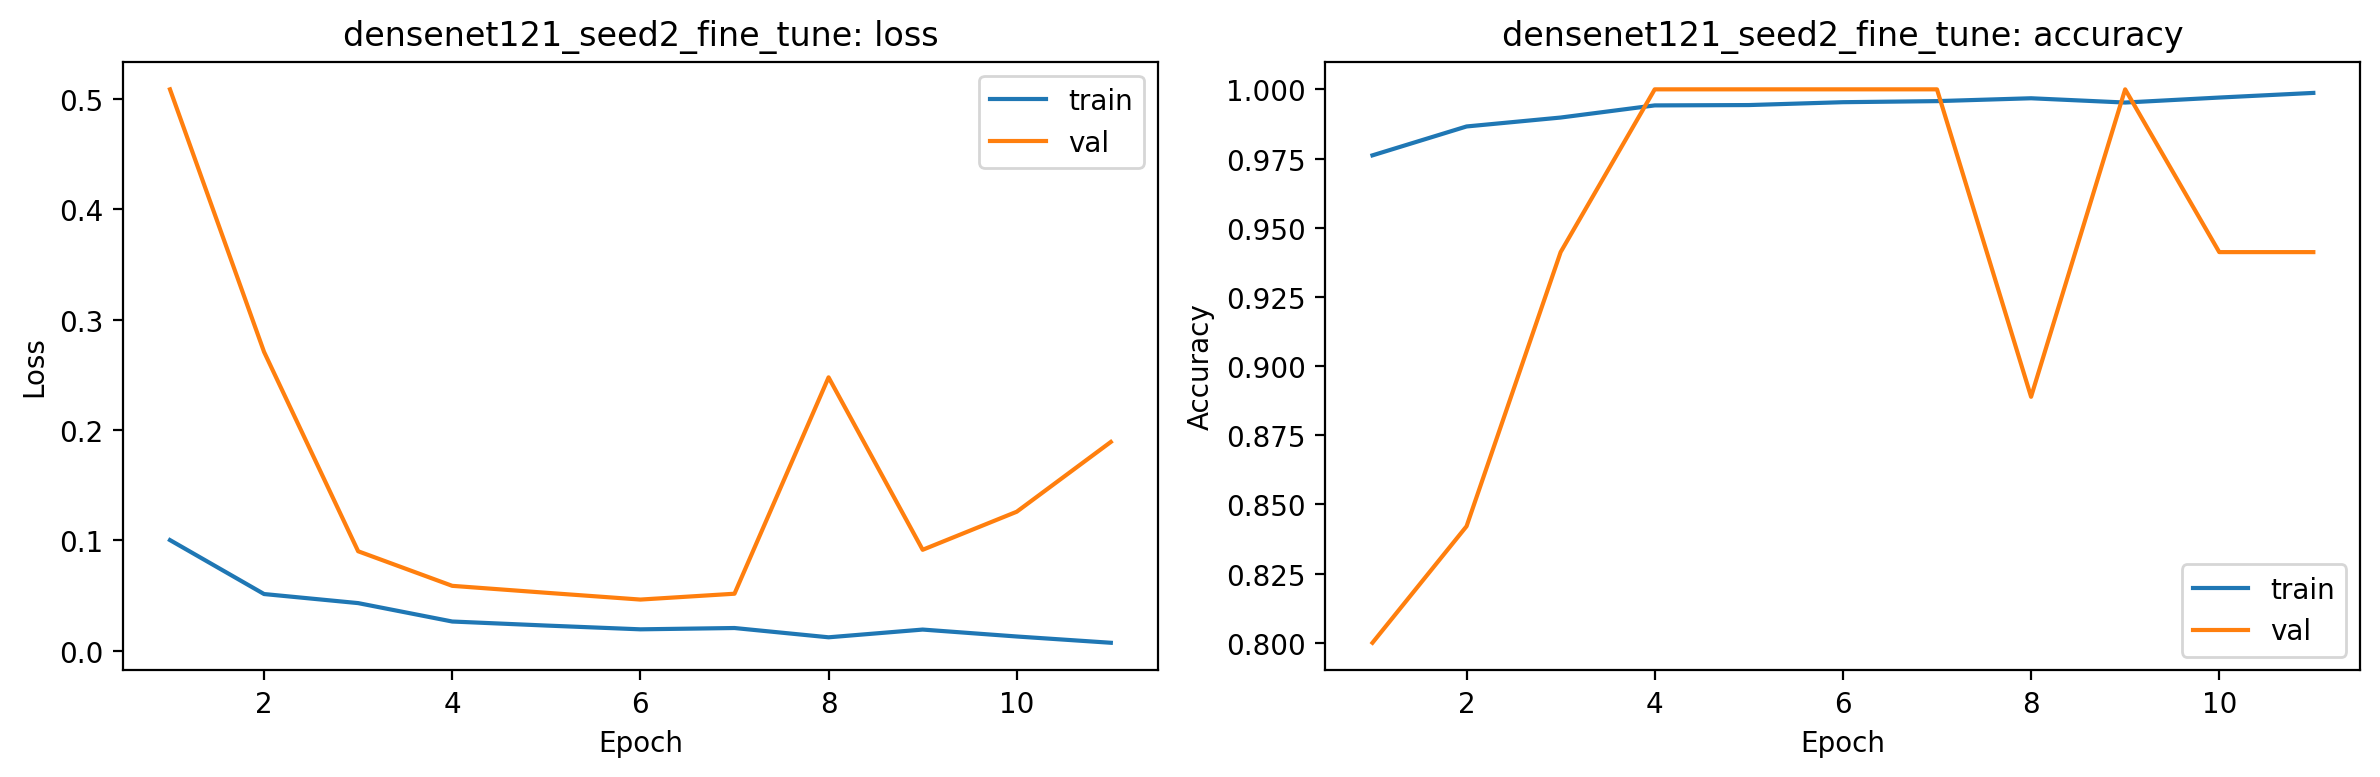
\includegraphics[width=\textwidth]{densenet121_seed2_fine_tune_training_curves.png}
\caption{densenet121 seed2 fine tune training curves}
\end{subfigure}
\caption{Binary training curves (per seed and phase), all models.}
\label{fig:app_curb}
\end{figure}
\FloatBarrier

\begin{figure}[h]
\centering
\begin{subfigure}{0.45\textwidth}
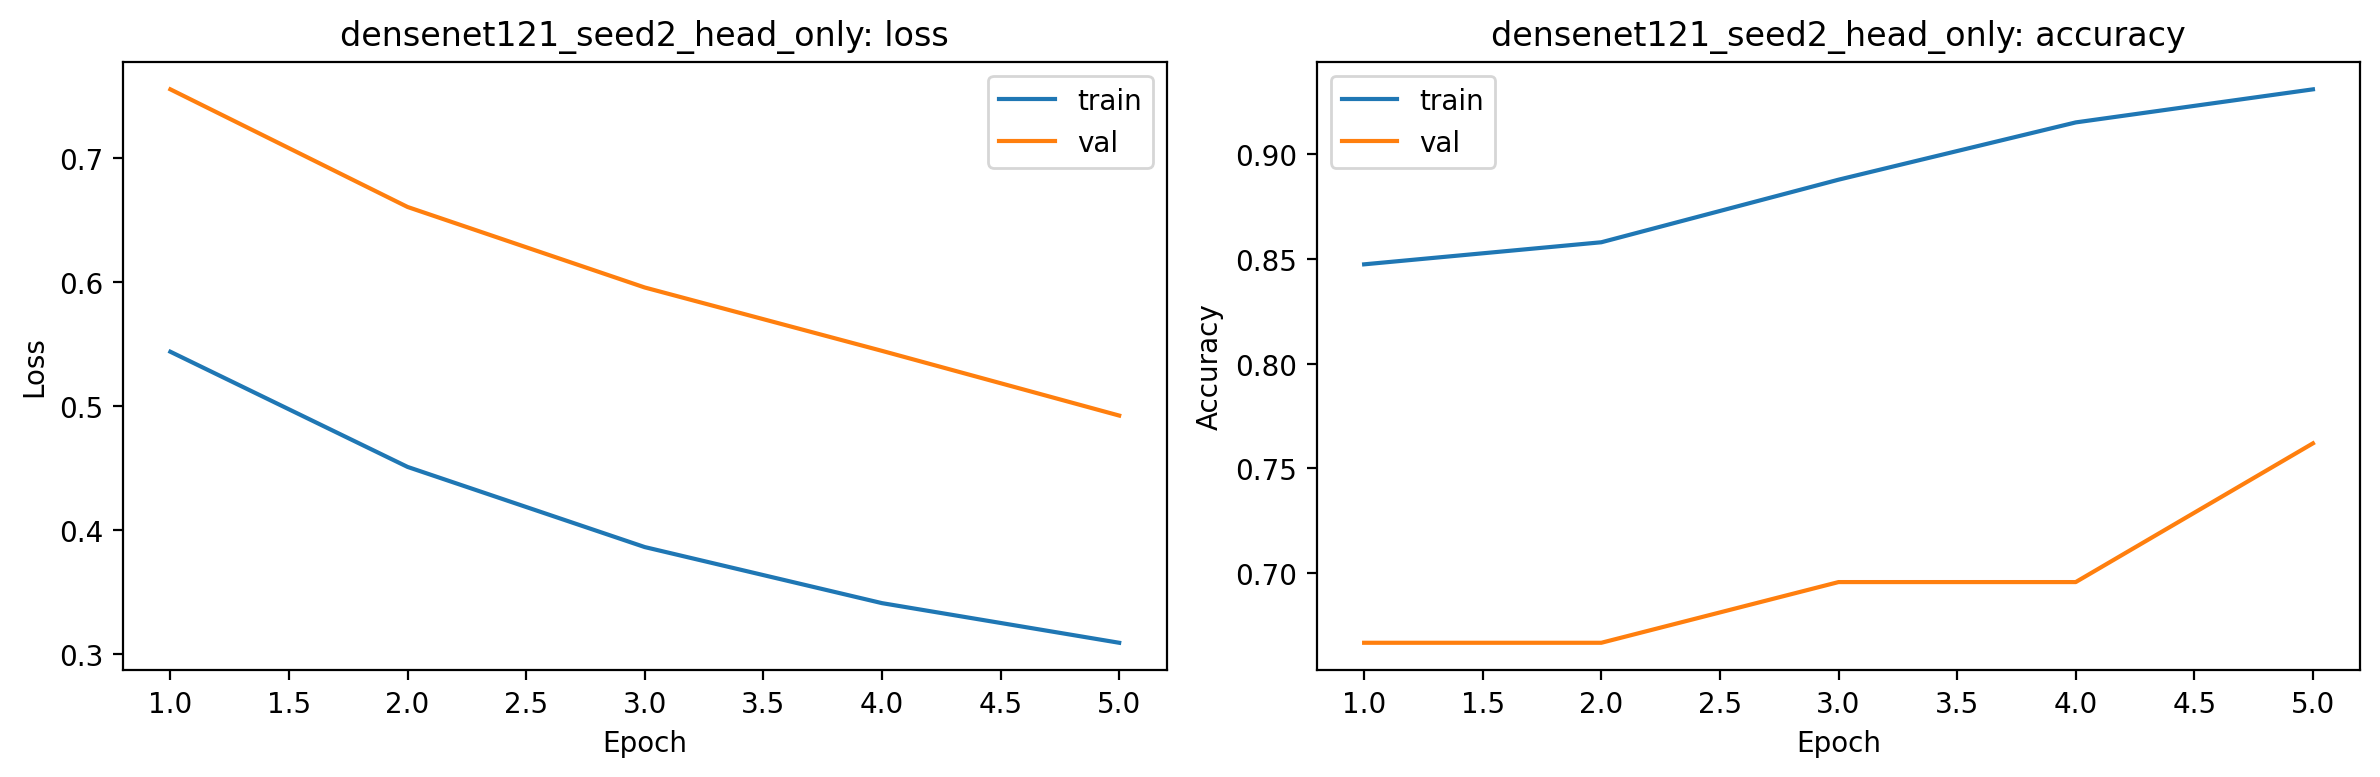
\includegraphics[width=\textwidth]{densenet121_seed2_head_only_training_curves.png}
\caption{densenet121 seed2 head only training curves}
\end{subfigure}\hfill
\begin{subfigure}{0.45\textwidth}
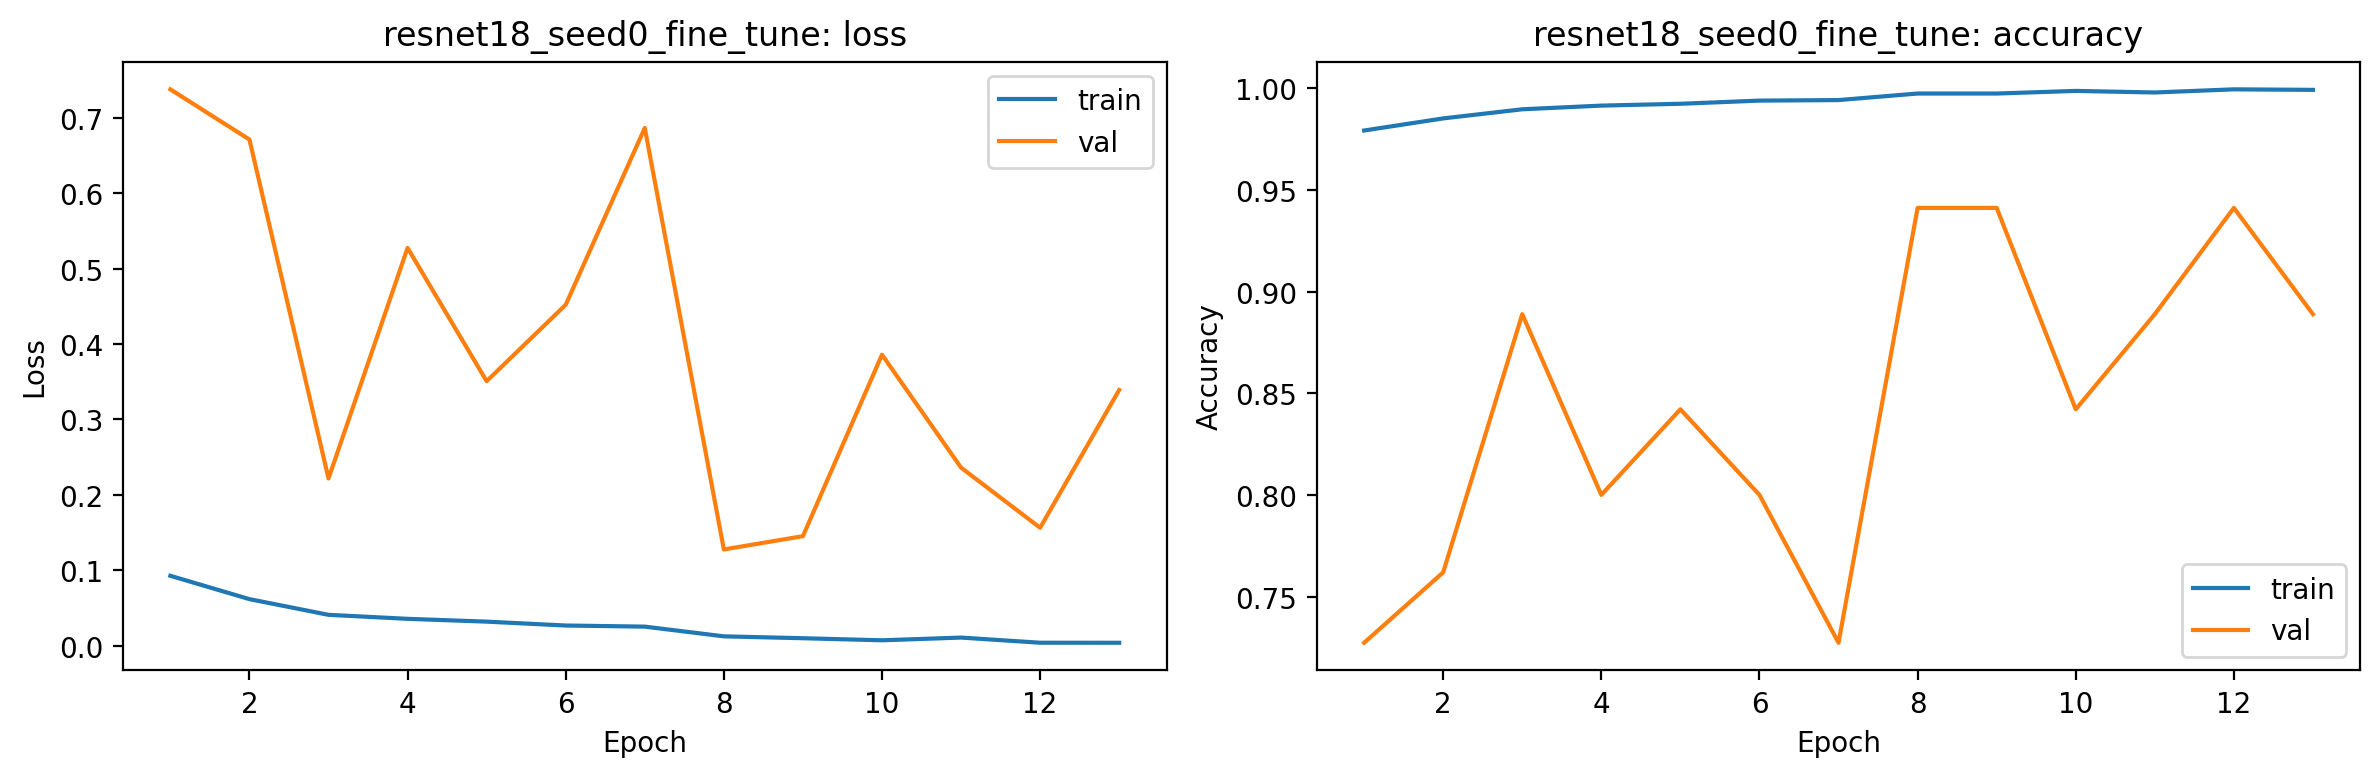
\includegraphics[width=\textwidth]{resnet18_seed0_fine_tune_training_curves.png}
\caption{resnet18 seed0 fine tune training curves}
\end{subfigure}\\[0.6em]
\begin{subfigure}{0.45\textwidth}
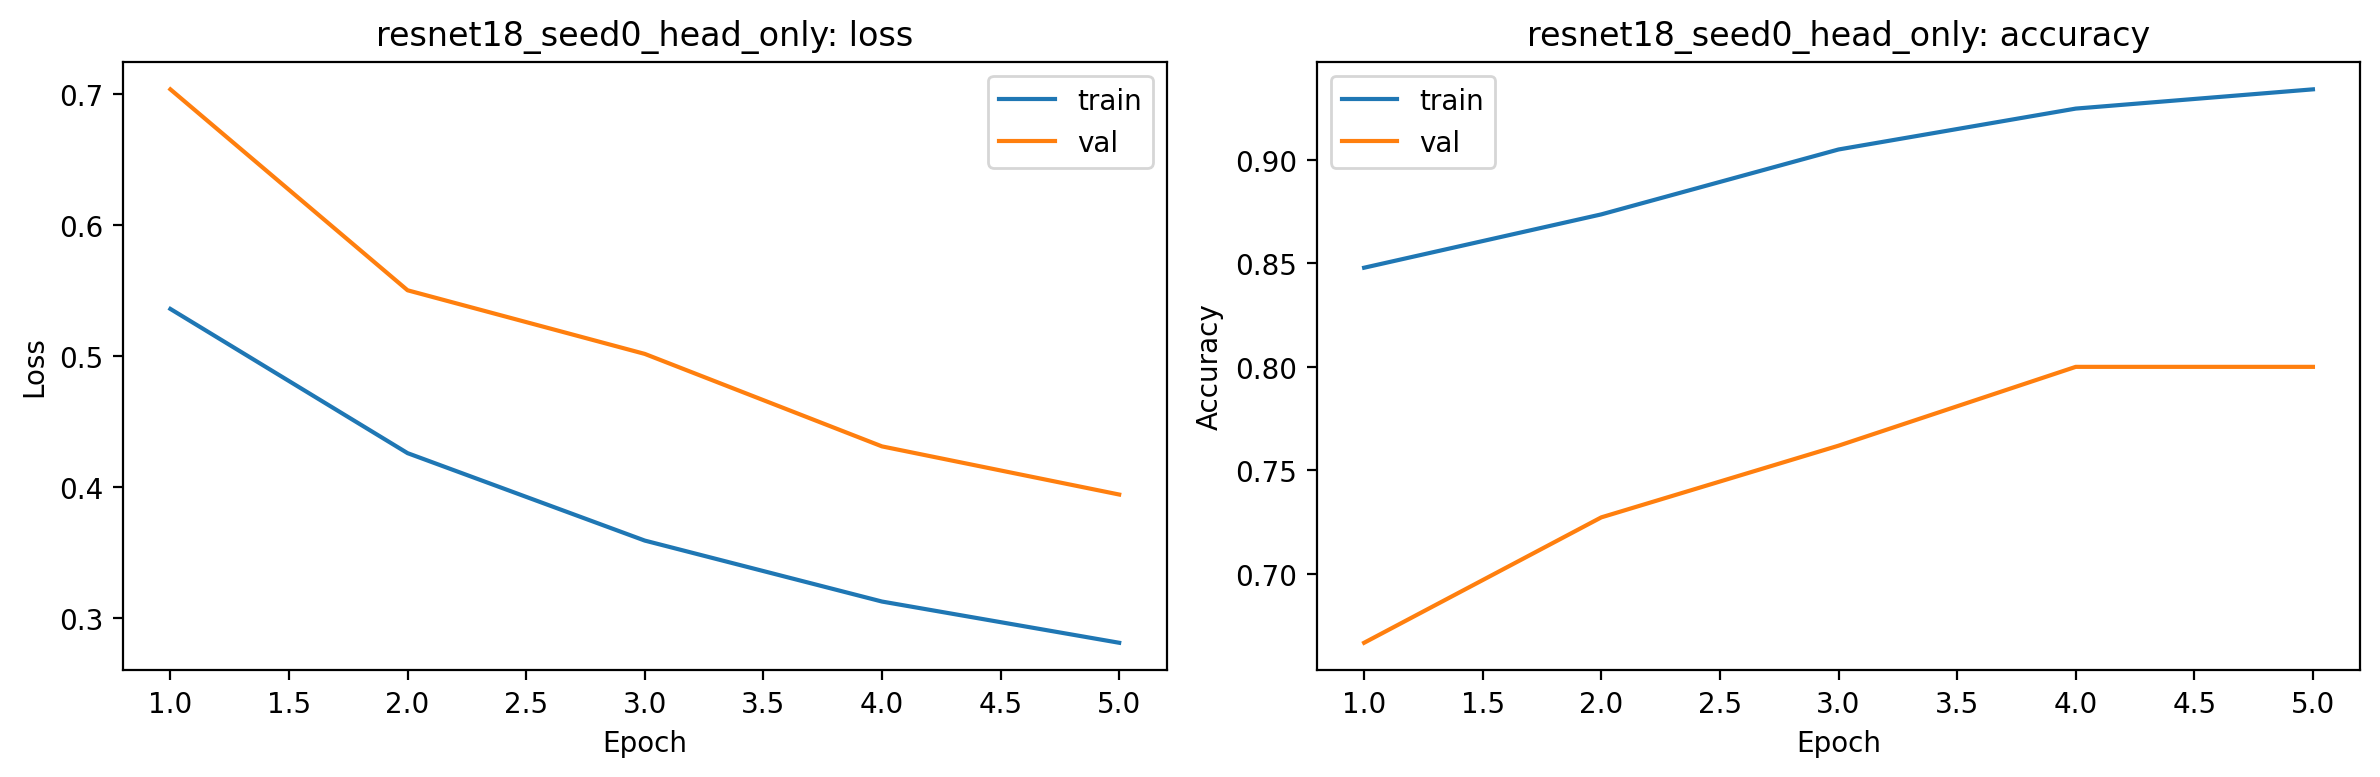
\includegraphics[width=\textwidth]{resnet18_seed0_head_only_training_curves.png}
\caption{resnet18 seed0 head only training curves}
\end{subfigure}\hfill
\begin{subfigure}{0.45\textwidth}
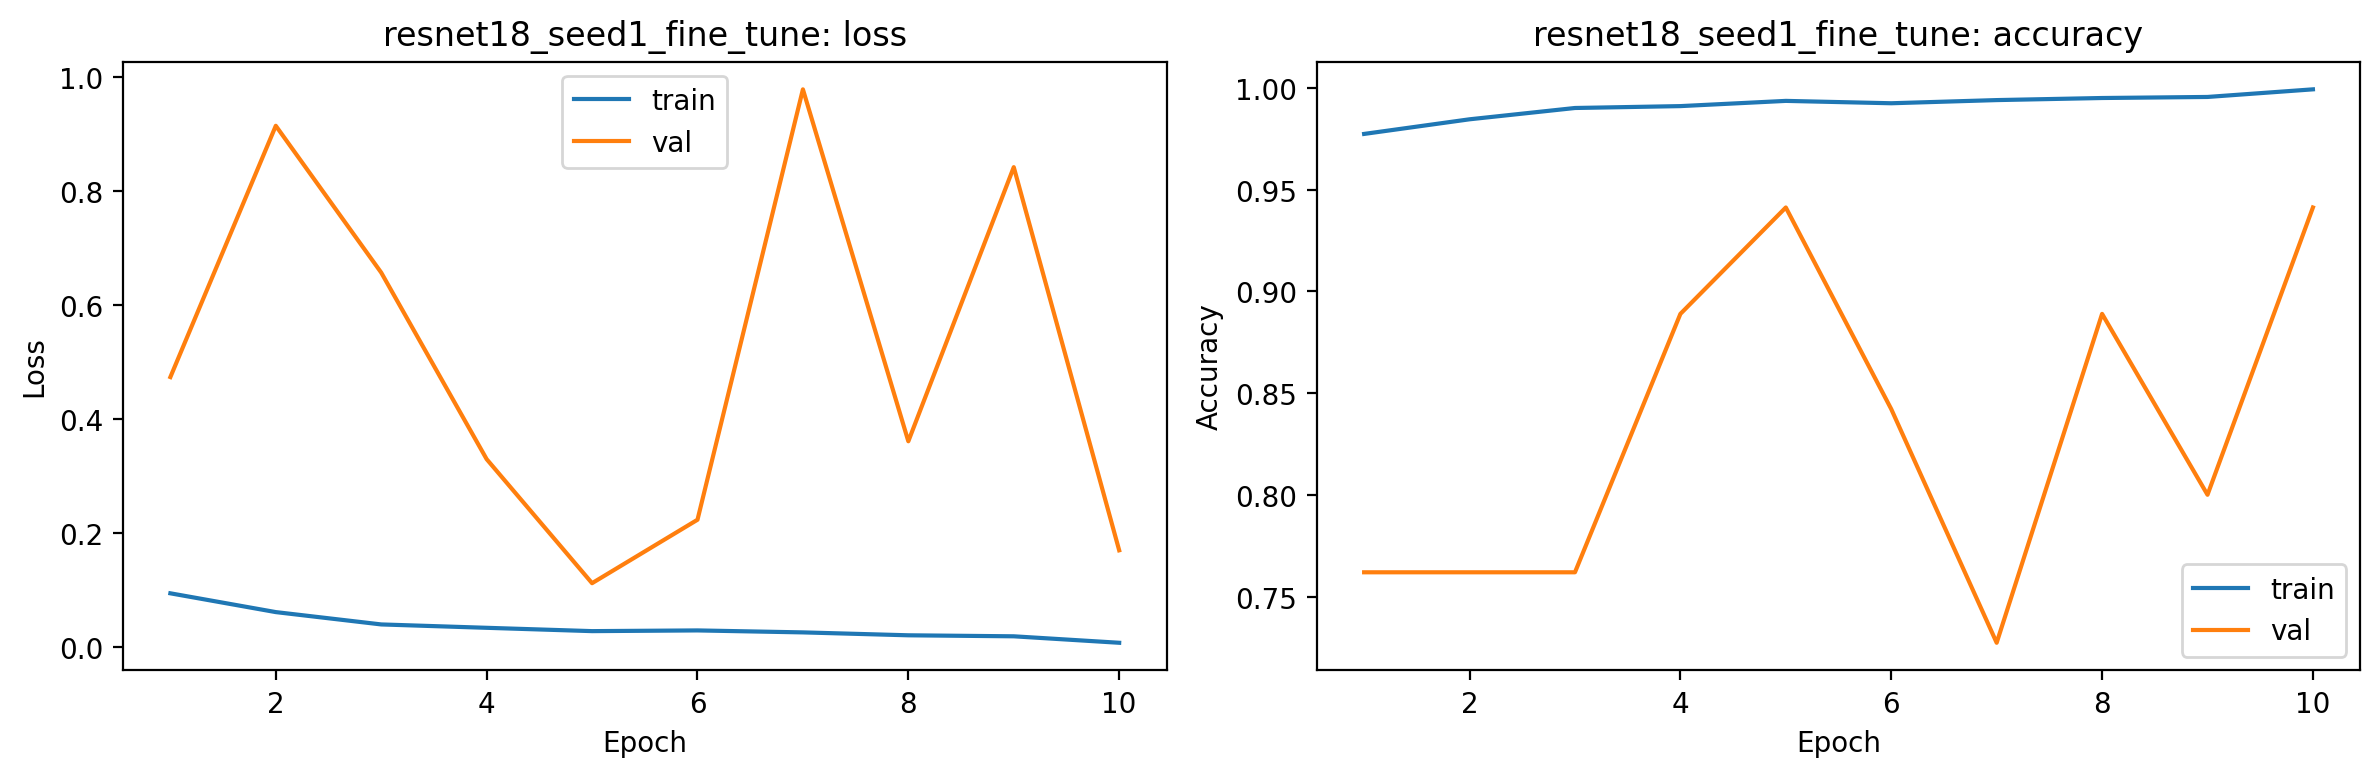
\includegraphics[width=\textwidth]{resnet18_seed1_fine_tune_training_curves.png}
\caption{resnet18 seed1 fine tune training curves}
\end{subfigure}\\[0.6em]
\begin{subfigure}{0.45\textwidth}
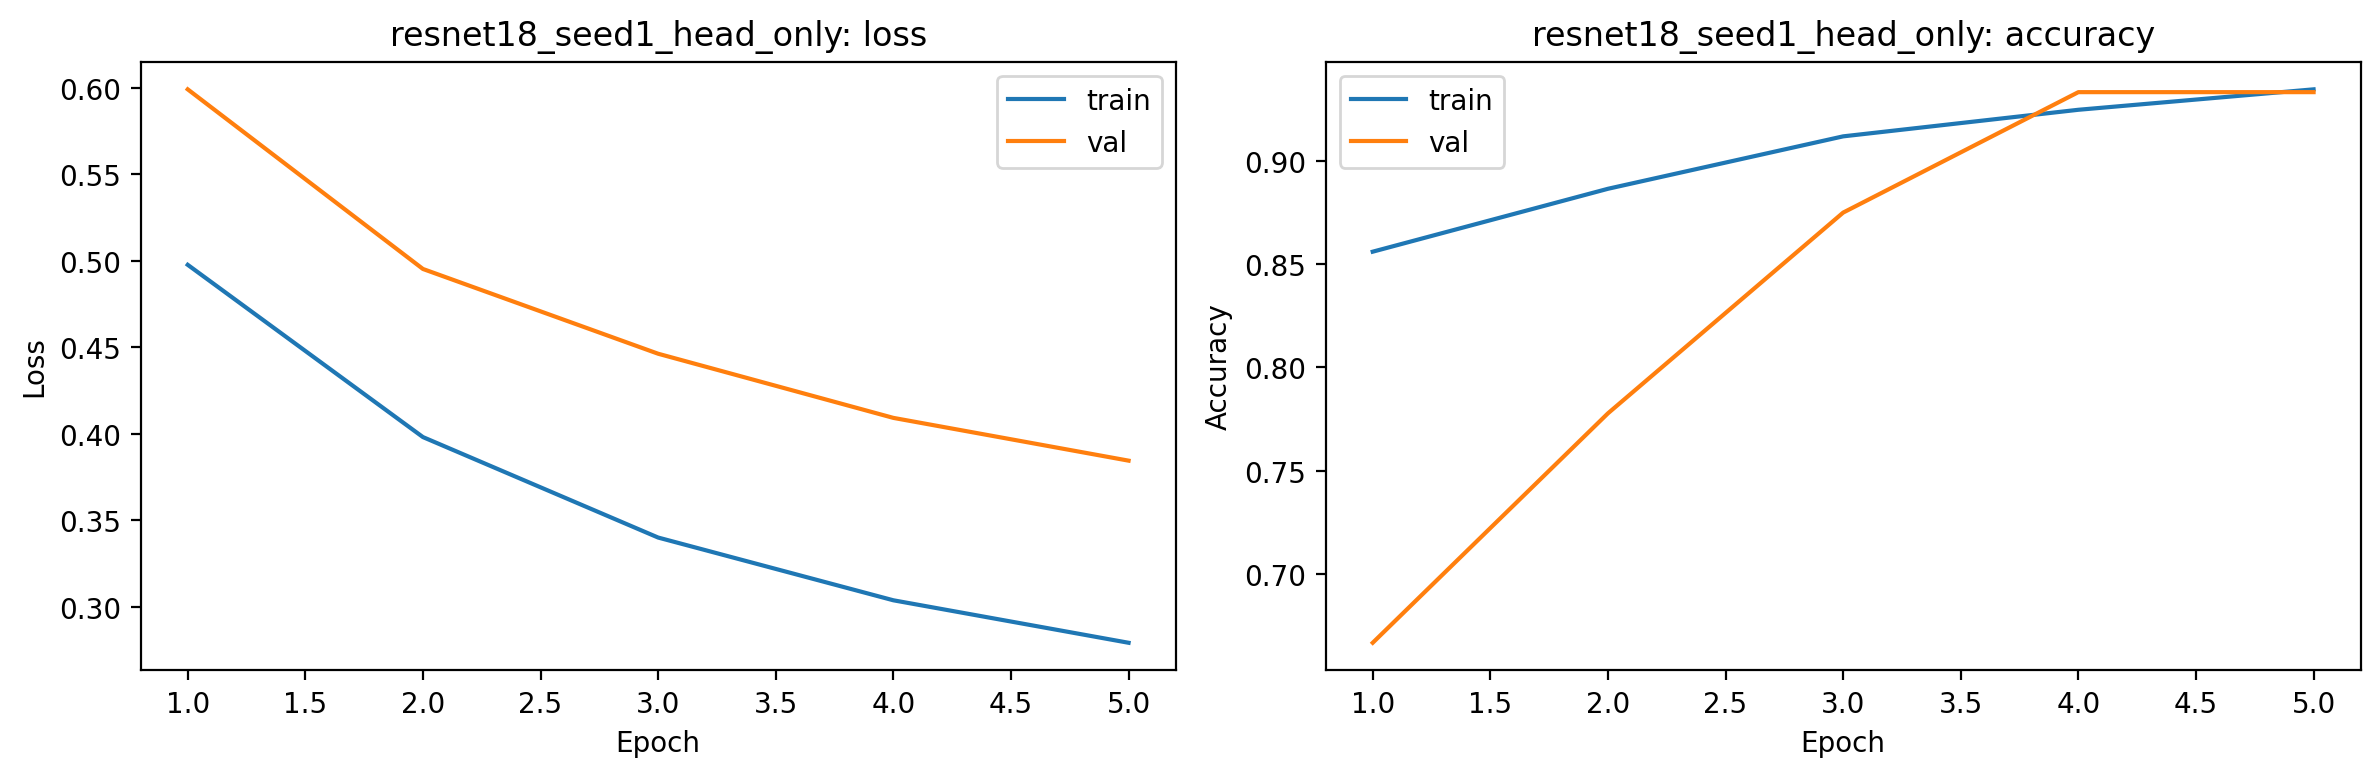
\includegraphics[width=\textwidth]{resnet18_seed1_head_only_training_curves.png}
\caption{resnet18 seed1 head only training curves}
\end{subfigure}\hfill
\begin{subfigure}{0.45\textwidth}
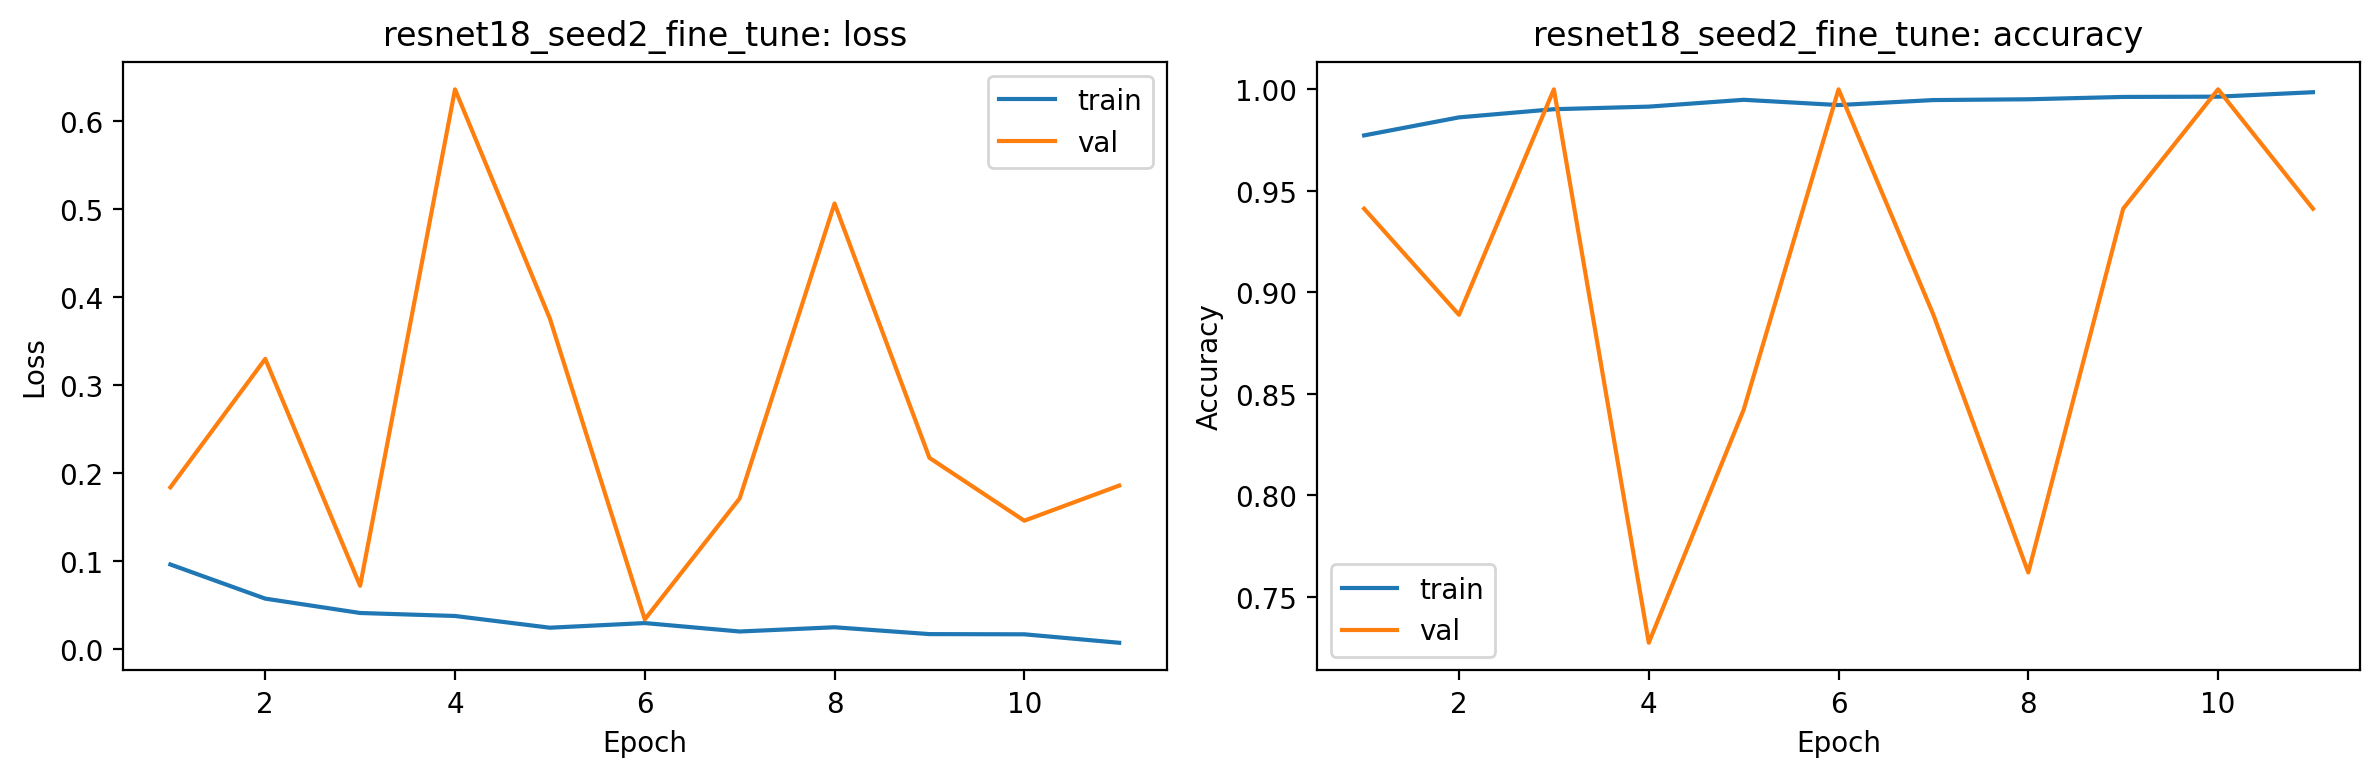
\includegraphics[width=\textwidth]{resnet18_seed2_fine_tune_training_curves.png}
\caption{resnet18 seed2 fine tune training curves}
\end{subfigure}\\[0.6em]
\begin{subfigure}{0.45\textwidth}
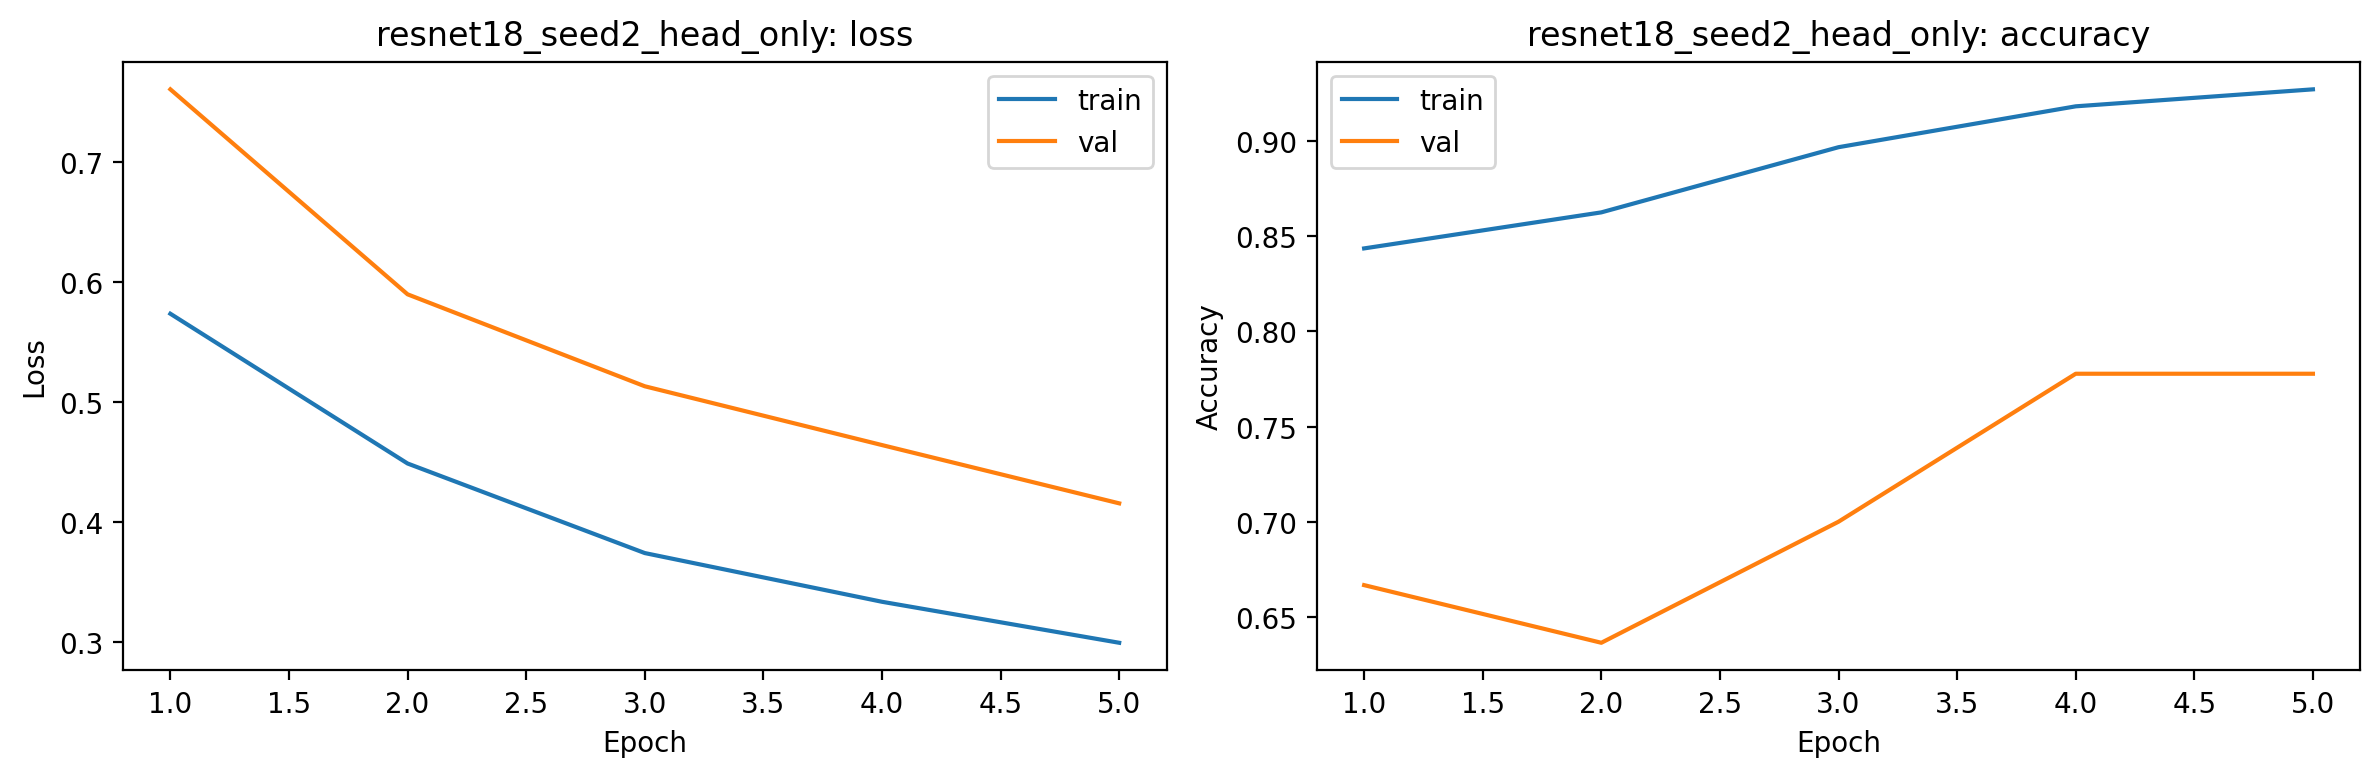
\includegraphics[width=\textwidth]{resnet18_seed2_head_only_training_curves.png}
\caption{resnet18 seed2 head only training curves}
\end{subfigure}\hfill
\begin{subfigure}{0.45\textwidth}
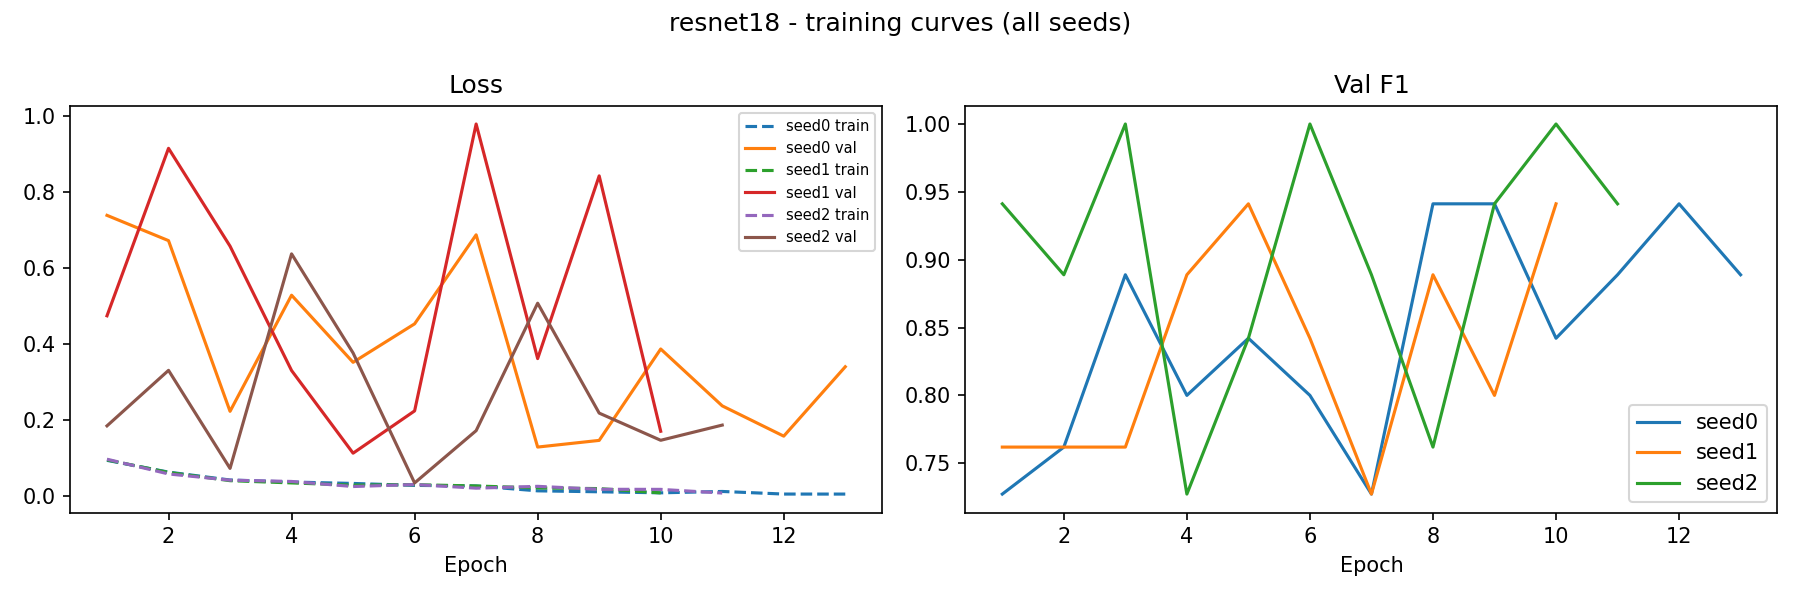
\includegraphics[width=\textwidth]{resnet18_training_curves.png}
\caption{resnet18 training curves}
\end{subfigure}
\caption{Binary training curves (per seed and phase), all models. (continued)}
\label{fig:app_curb_1}
\end{figure}
\FloatBarrier

\begin{figure}[h]
\centering
\begin{subfigure}{0.31\textwidth}
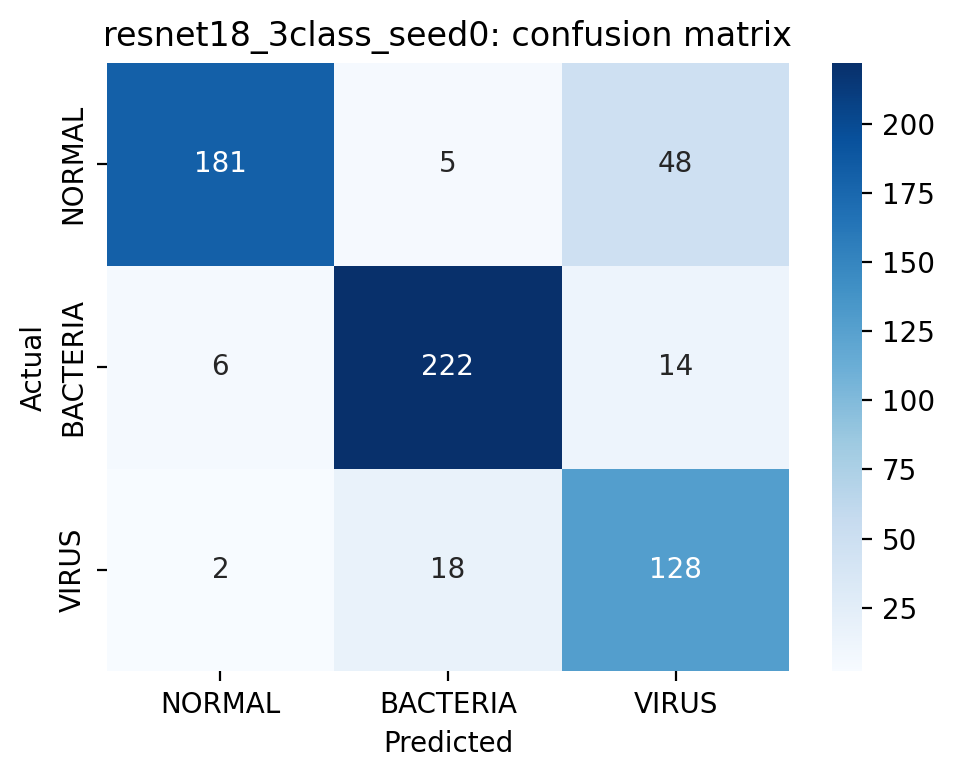
\includegraphics[width=\textwidth]{resnet18_3class_seed0_confusion_matrix.png}
\caption{resnet18 3class seed0 confusion matrix}
\end{subfigure}\hfill
\begin{subfigure}{0.31\textwidth}
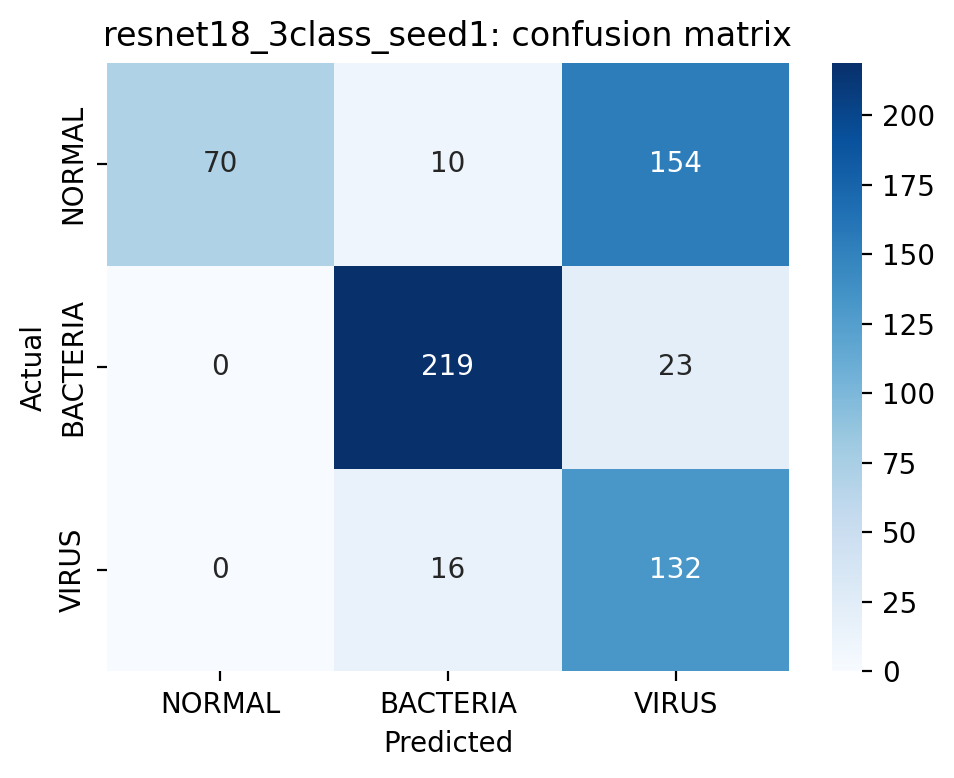
\includegraphics[width=\textwidth]{resnet18_3class_seed1_confusion_matrix.png}
\caption{resnet18 3class seed1 confusion matrix}
\end{subfigure}\hfill
\begin{subfigure}{0.31\textwidth}
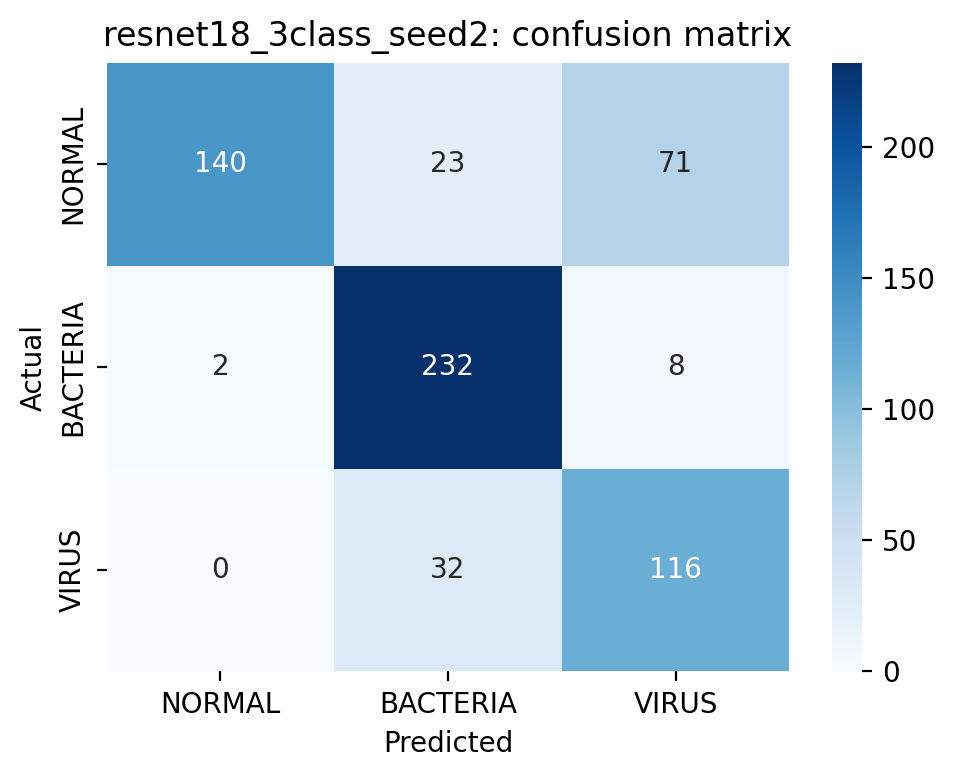
\includegraphics[width=\textwidth]{resnet18_3class_seed2_confusion_matrix.png}
\caption{resnet18 3class seed2 confusion matrix}
\end{subfigure}
\caption{Three-class confusion matrices for ResNet18 (per seed).}
\label{fig:app_cm3b}
\end{figure}
\FloatBarrier

\begin{figure}[h]
\centering
\begin{subfigure}{0.45\textwidth}
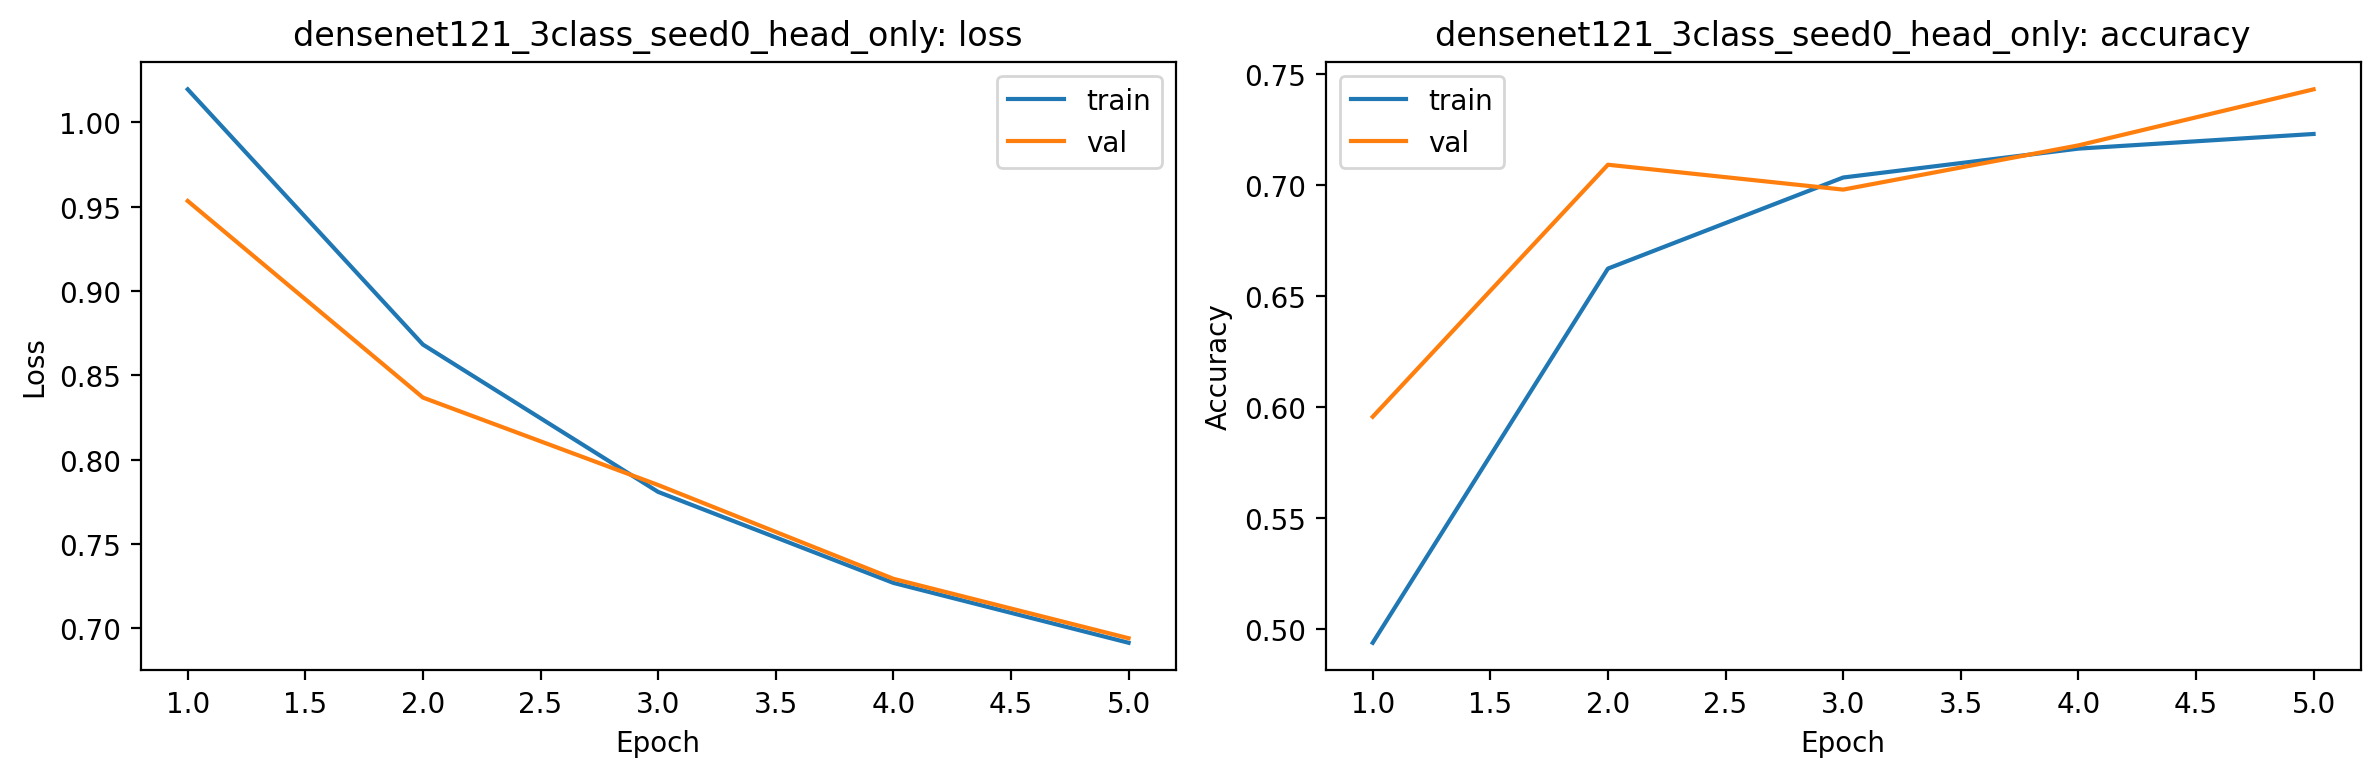
\includegraphics[width=\textwidth]{densenet121_3class_seed0_head_only_training_curves.png}
\caption{densenet121 3class seed0 head only training curves}
\end{subfigure}\hfill
\begin{subfigure}{0.45\textwidth}
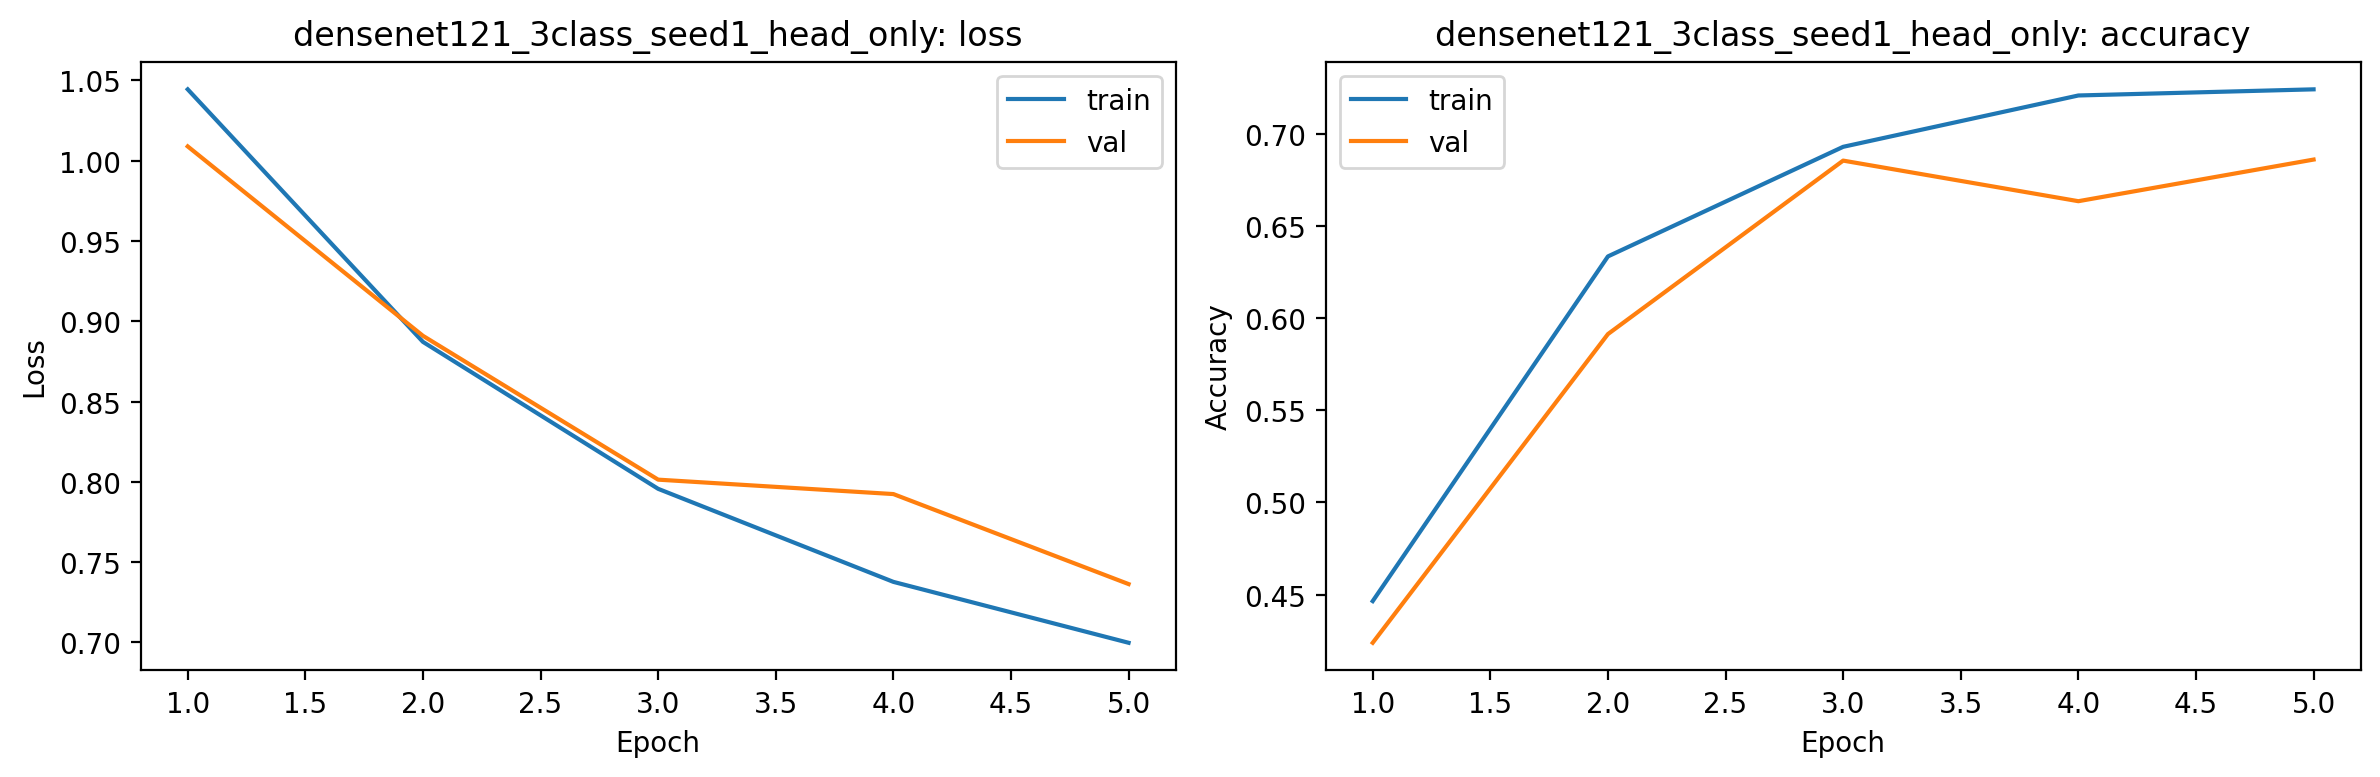
\includegraphics[width=\textwidth]{densenet121_3class_seed1_head_only_training_curves.png}
\caption{densenet121 3class seed1 head only training curves}
\end{subfigure}\\[0.6em]
\begin{subfigure}{0.45\textwidth}
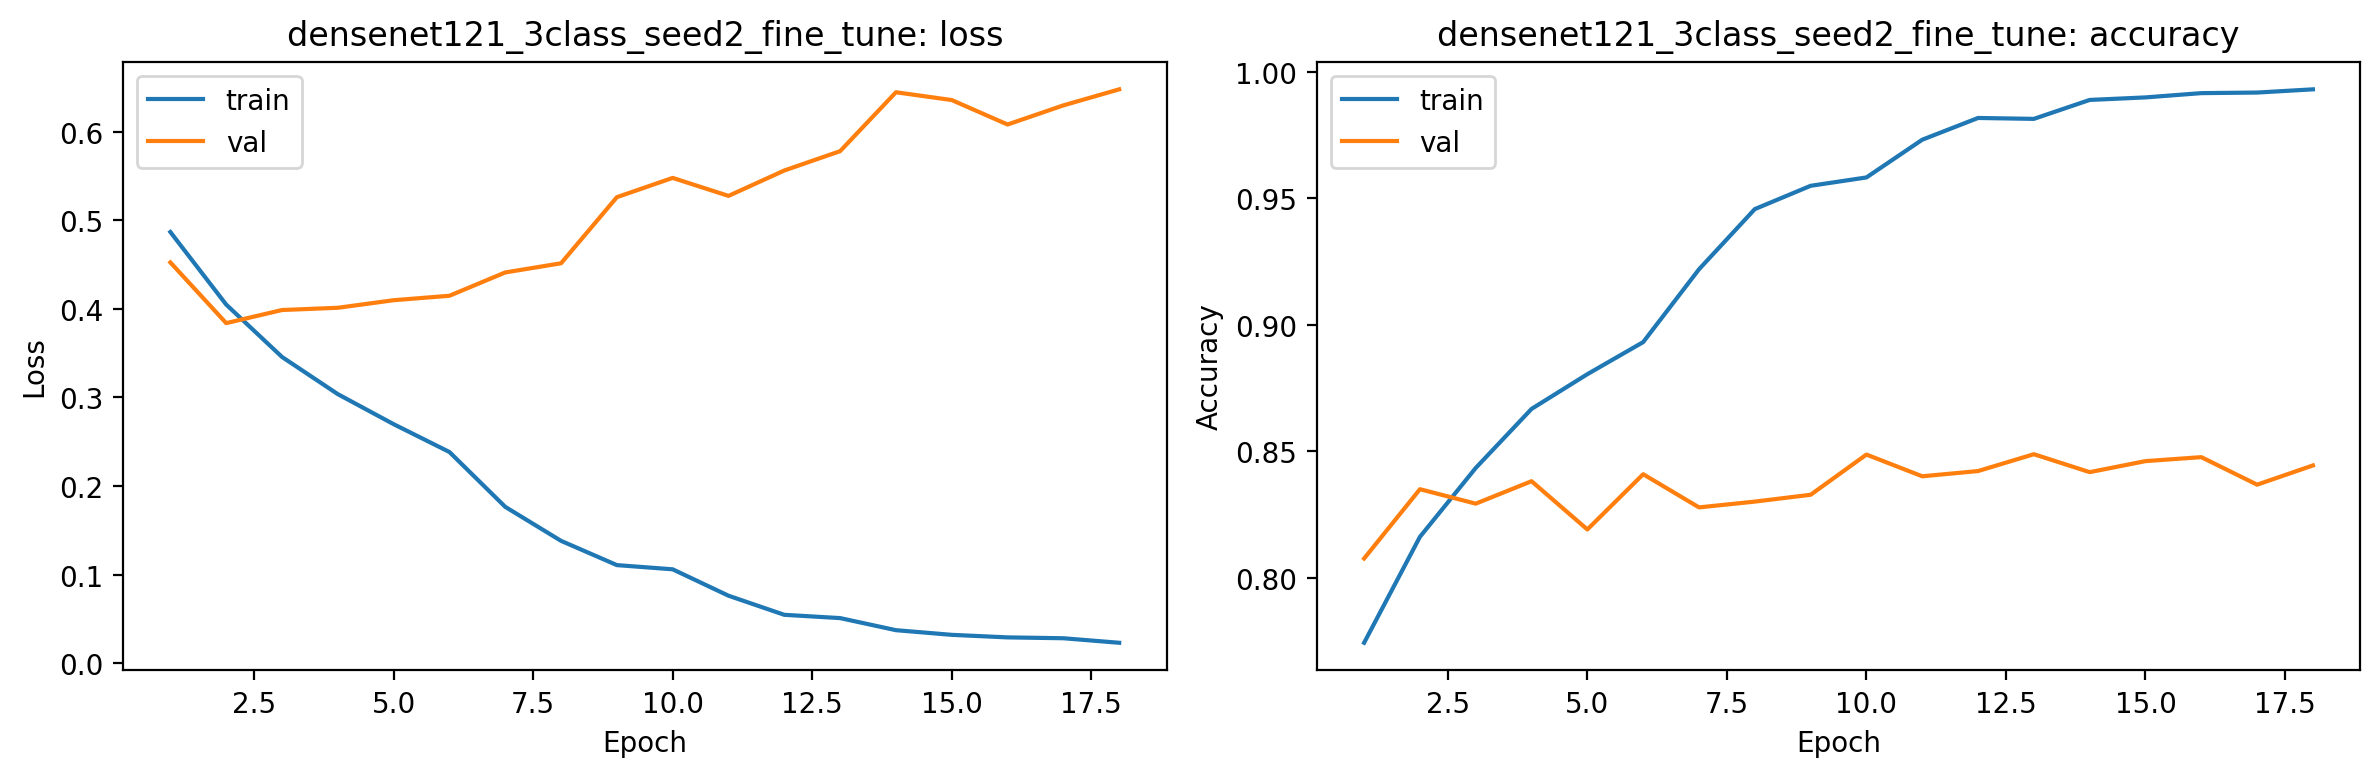
\includegraphics[width=\textwidth]{densenet121_3class_seed2_fine_tune_training_curves.png}
\caption{densenet121 3class seed2 fine tune training curves}
\end{subfigure}\hfill
\begin{subfigure}{0.45\textwidth}
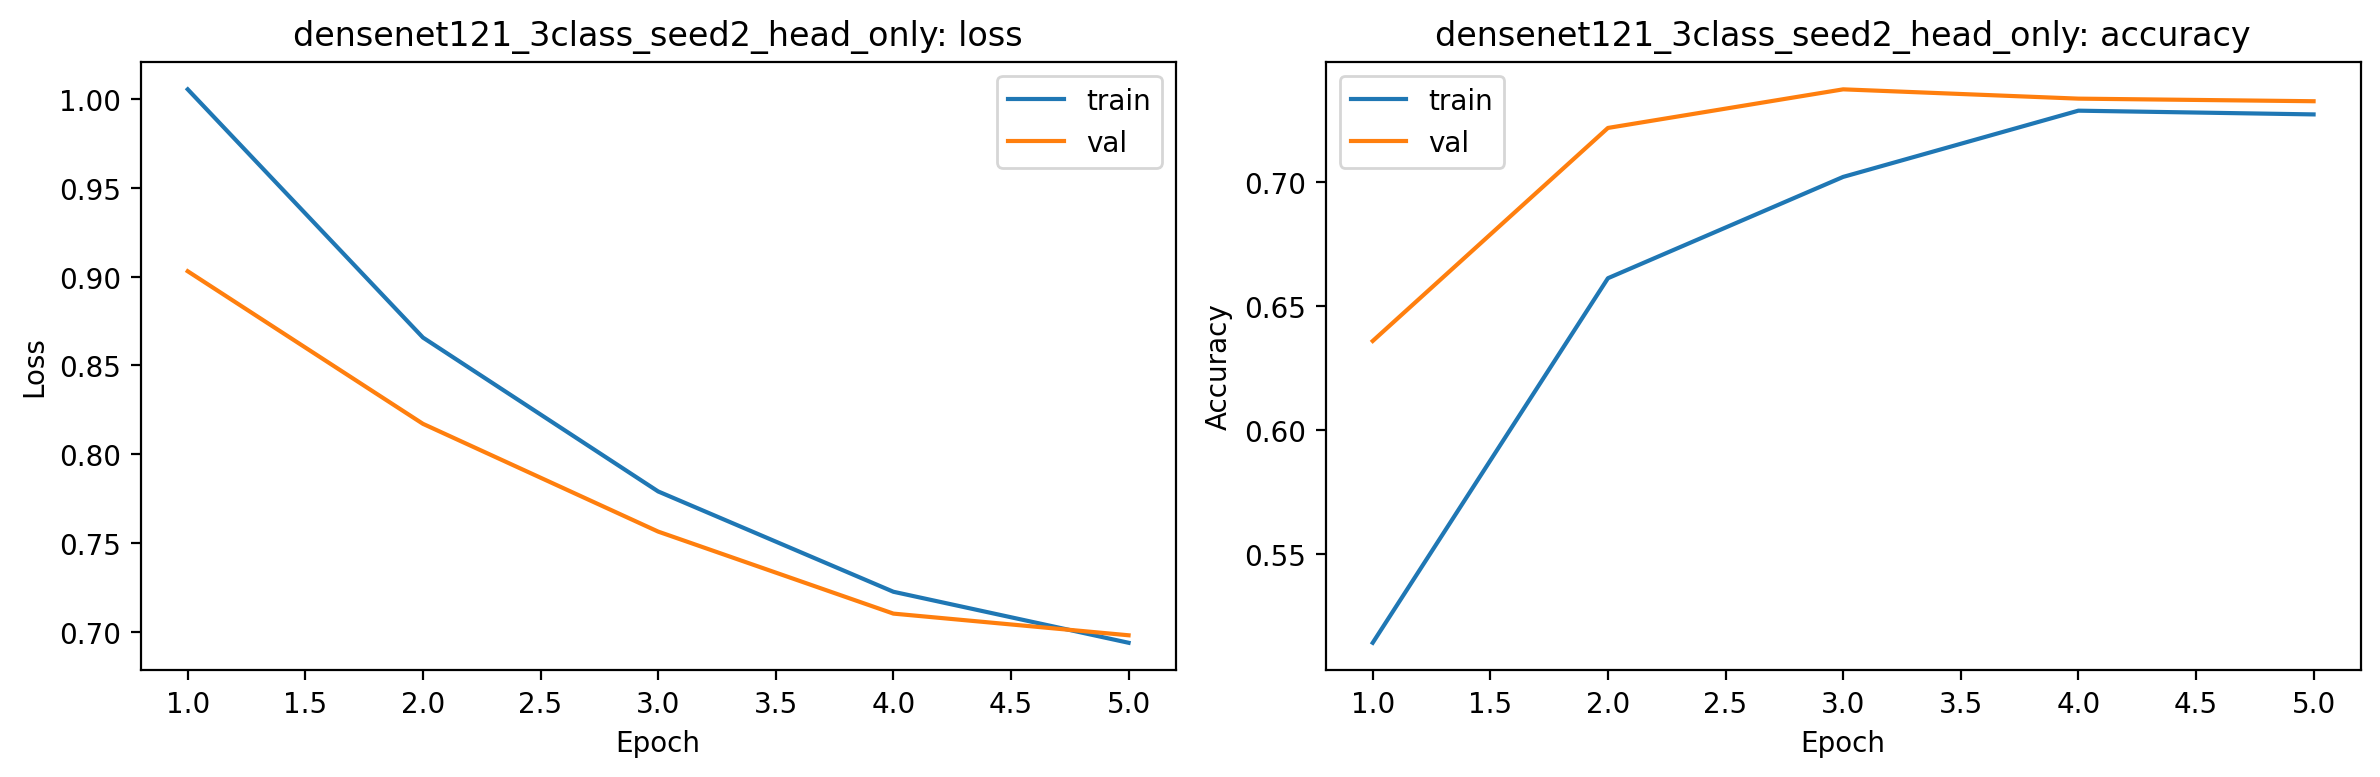
\includegraphics[width=\textwidth]{densenet121_3class_seed2_head_only_training_curves.png}
\caption{densenet121 3class seed2 head only training curves}
\end{subfigure}\\[0.6em]
\begin{subfigure}{0.45\textwidth}
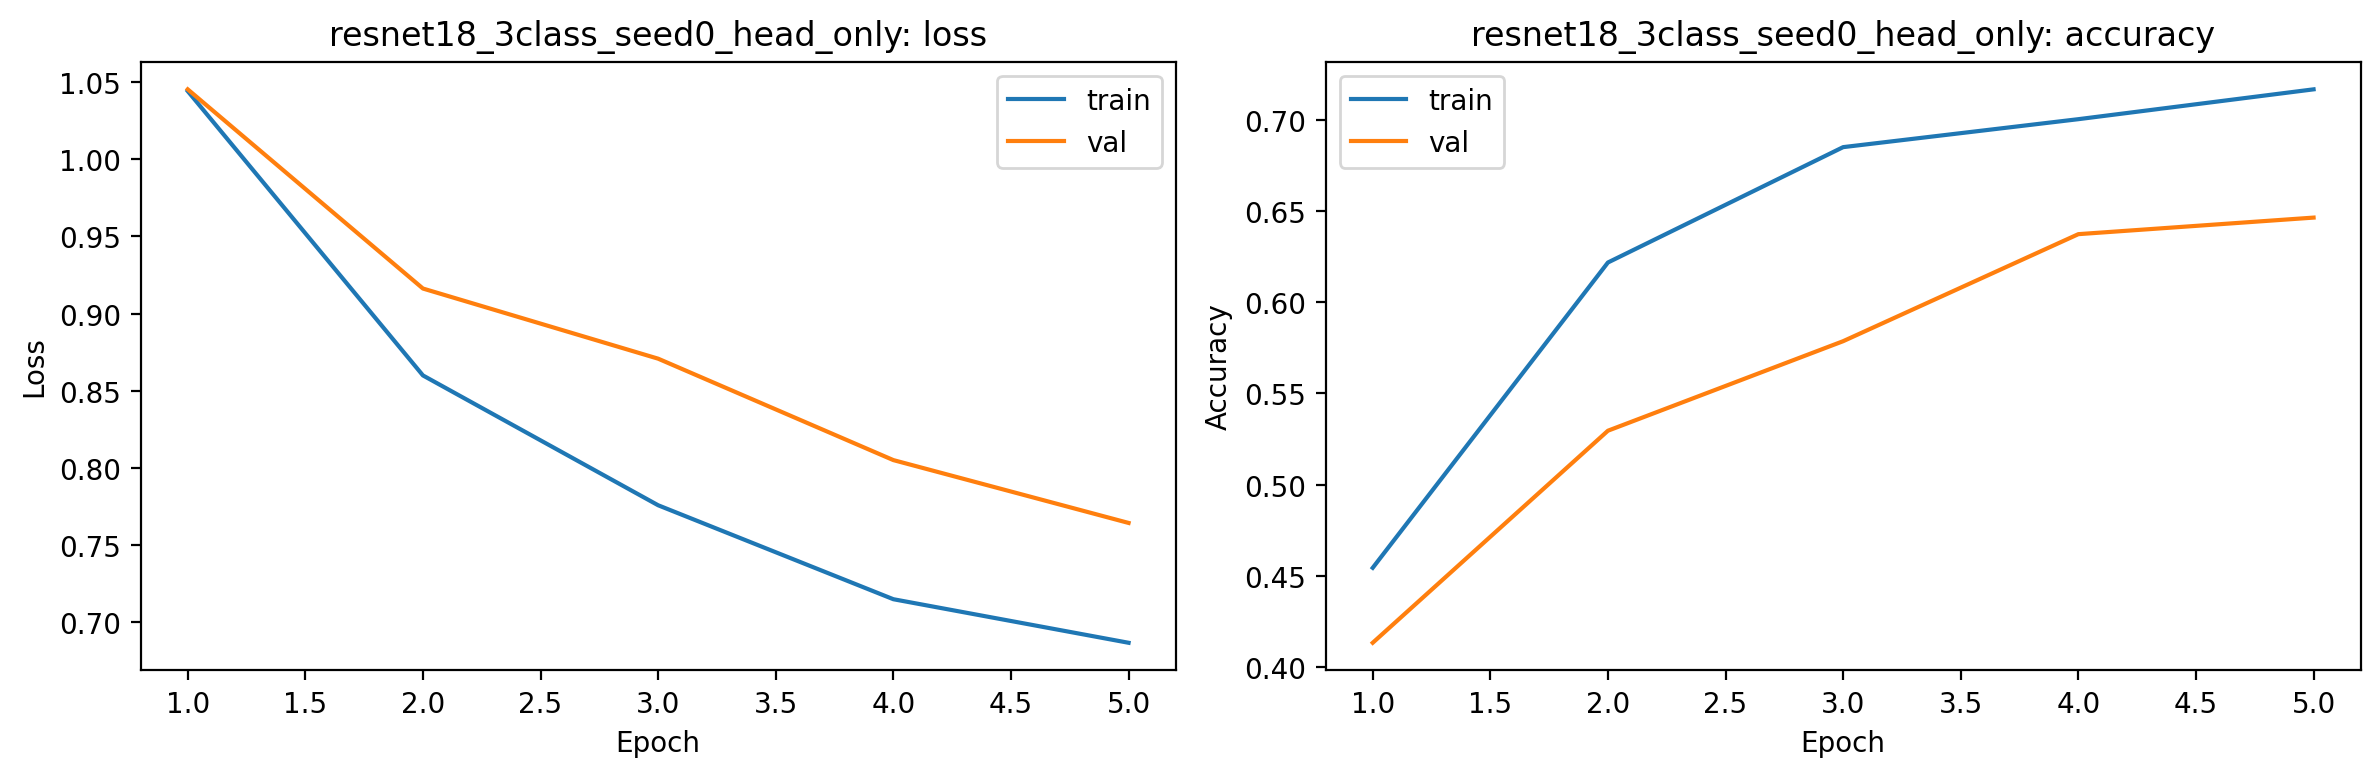
\includegraphics[width=\textwidth]{resnet18_3class_seed0_head_only_training_curves.png}
\caption{resnet18 3class seed0 head only training curves}
\end{subfigure}\hfill
\begin{subfigure}{0.45\textwidth}
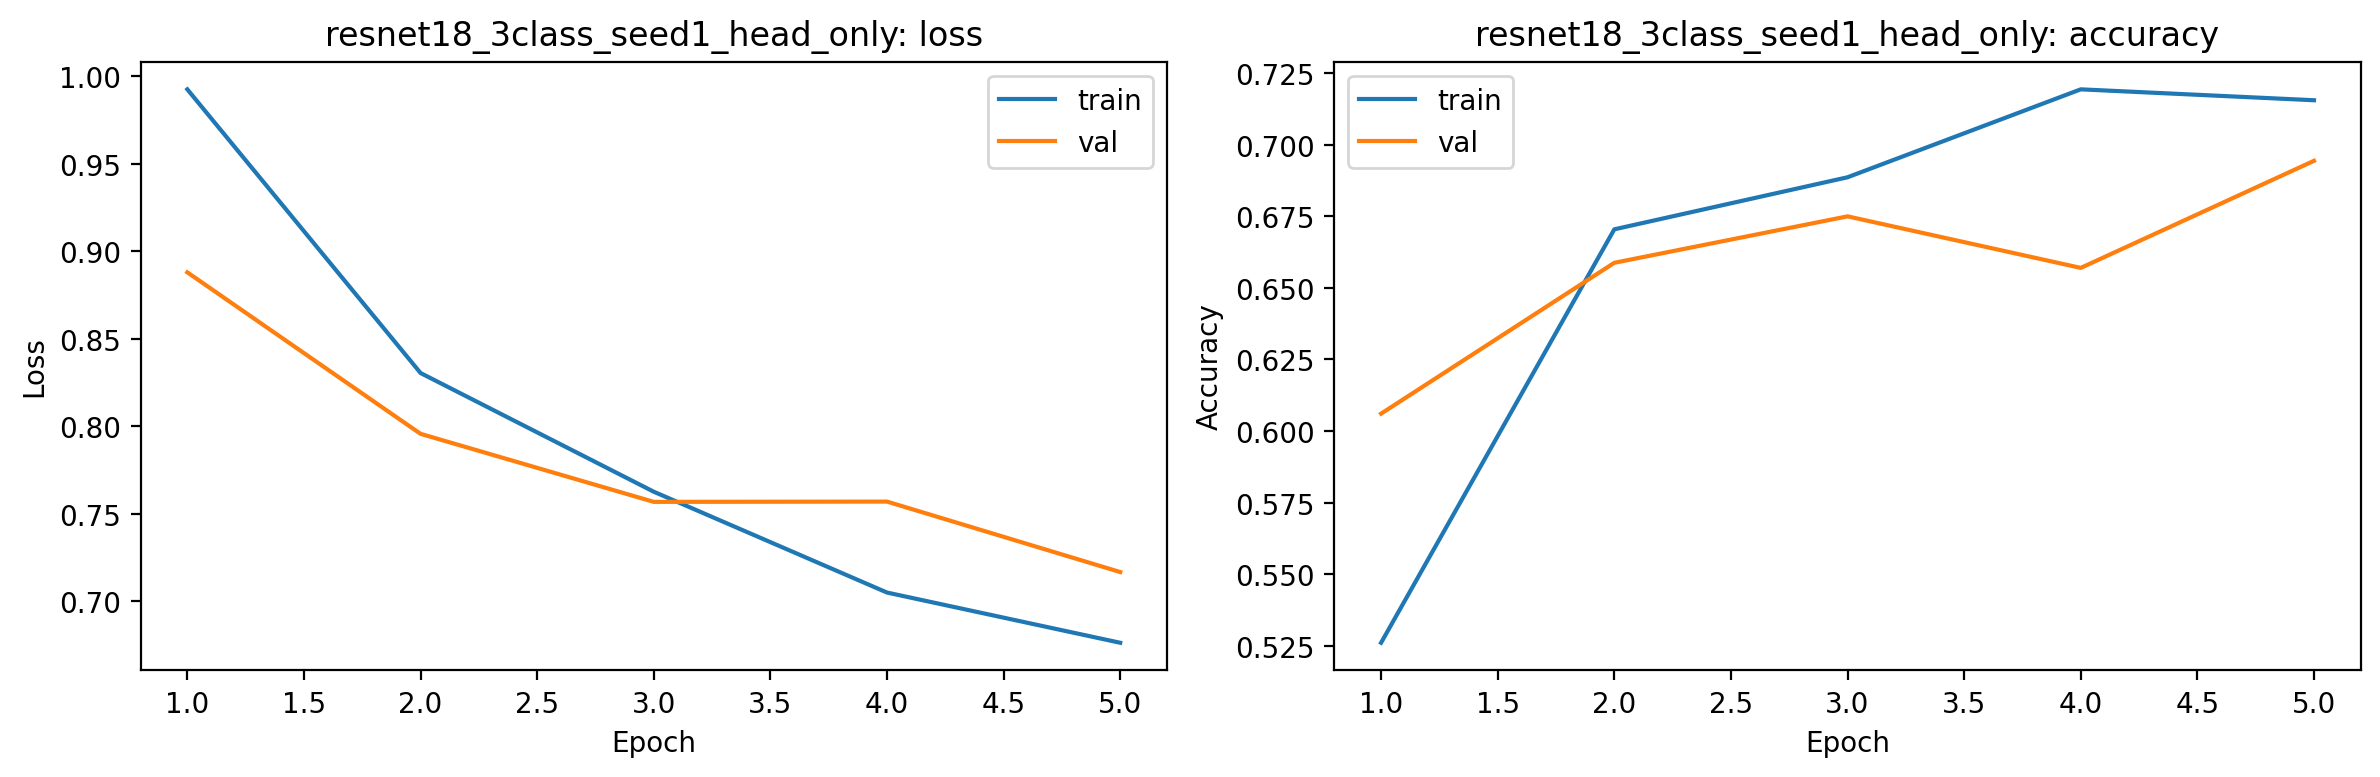
\includegraphics[width=\textwidth]{resnet18_3class_seed1_head_only_training_curves.png}
\caption{resnet18 3class seed1 head only training curves}
\end{subfigure}\\[0.6em]
\begin{subfigure}{0.45\textwidth}
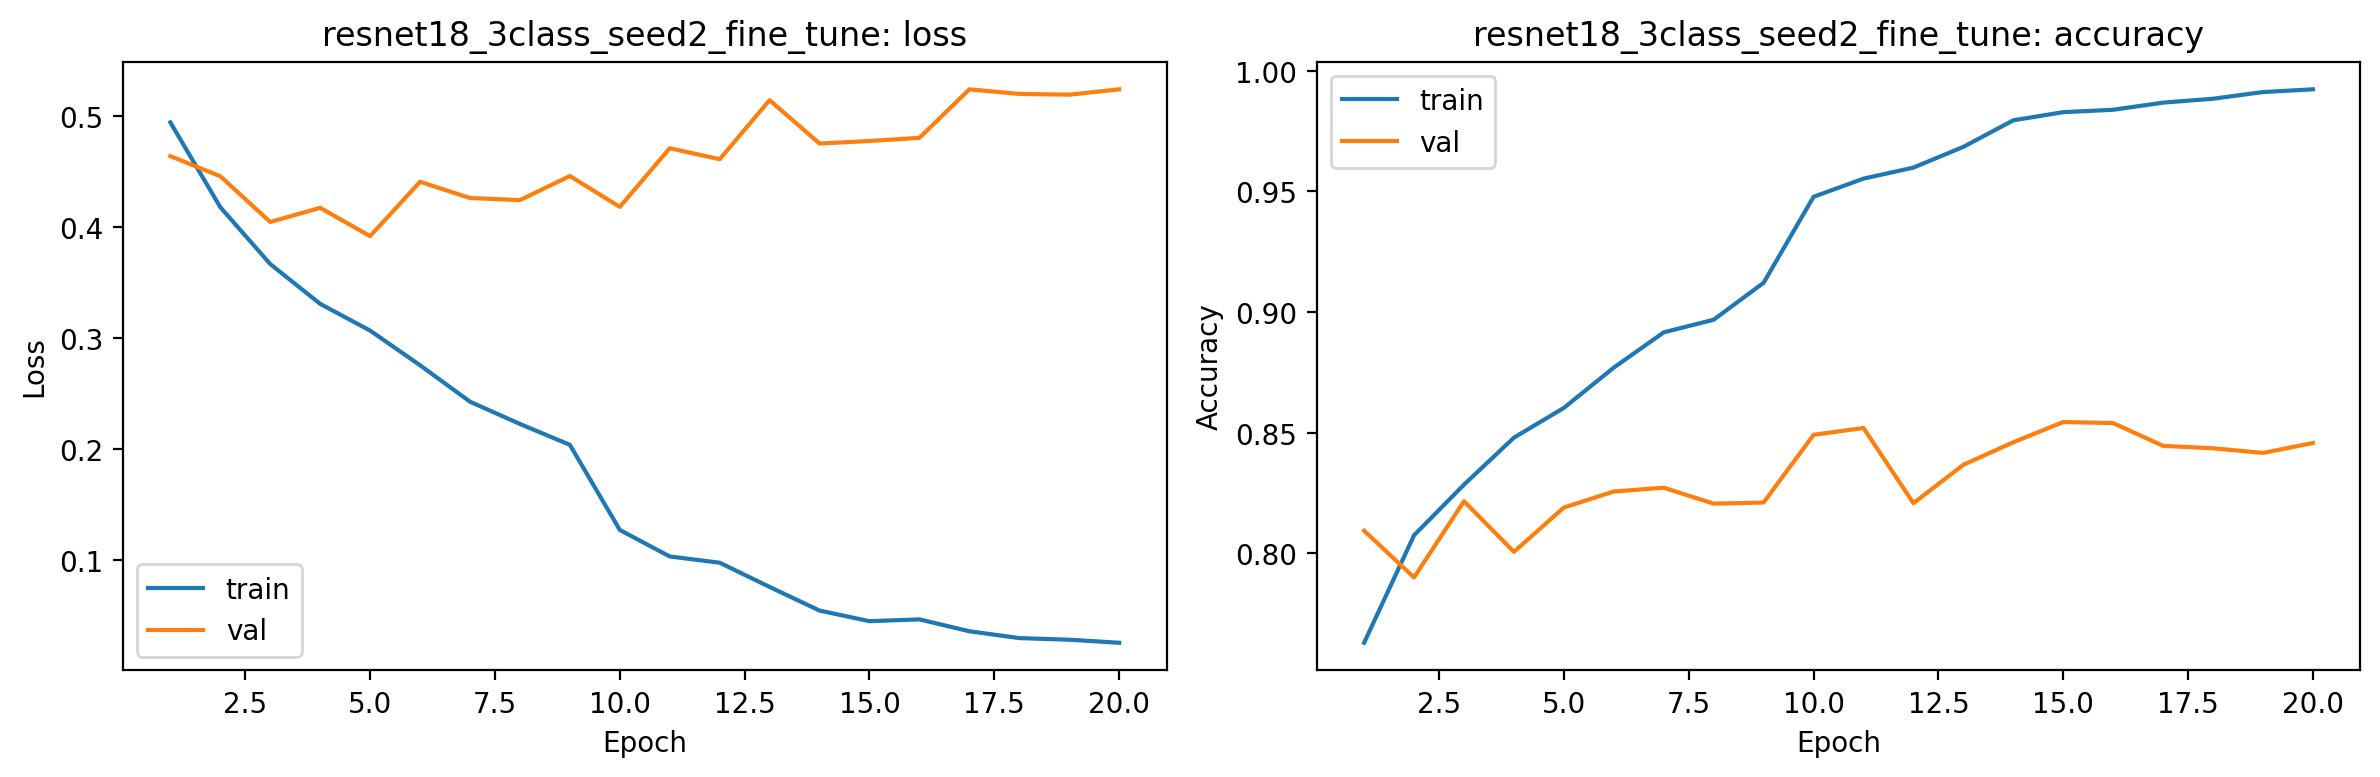
\includegraphics[width=\textwidth]{resnet18_3class_seed2_fine_tune_training_curves.png}
\caption{resnet18 3class seed2 fine tune training curves}
\end{subfigure}\hfill
\begin{subfigure}{0.45\textwidth}
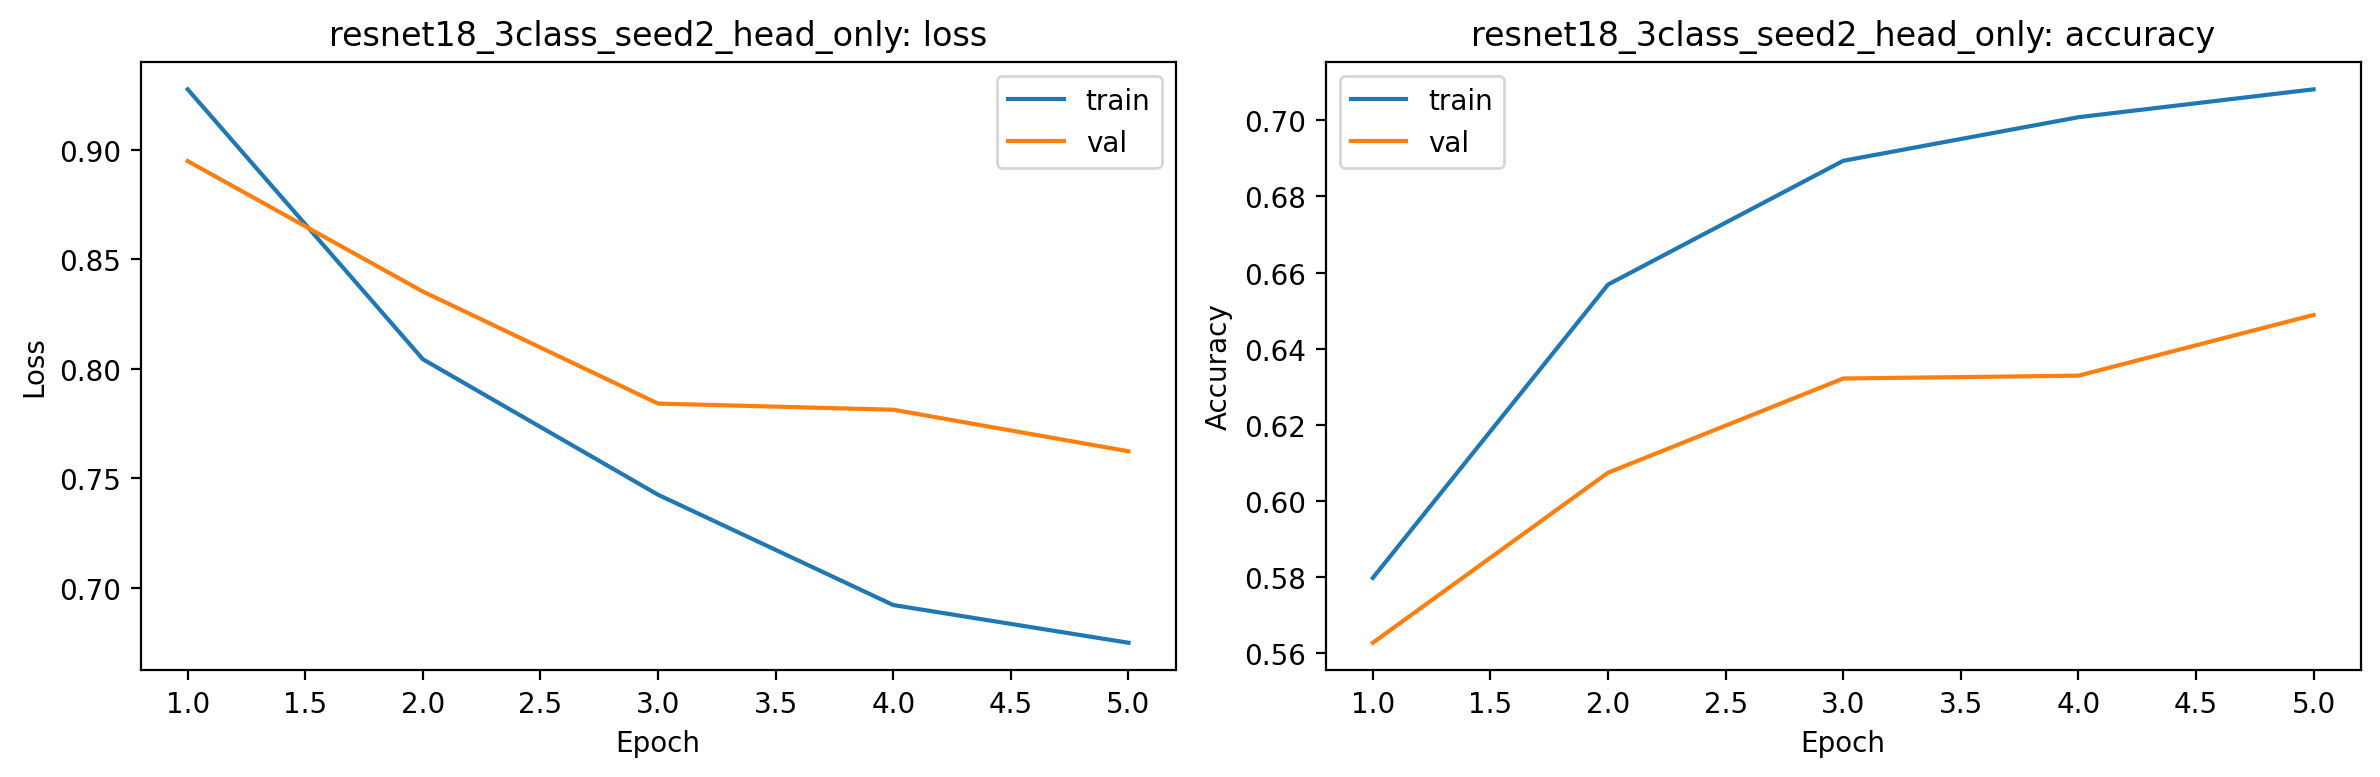
\includegraphics[width=\textwidth]{resnet18_3class_seed2_head_only_training_curves.png}
\caption{resnet18 3class seed2 head only training curves}
\end{subfigure}
\caption{Additional three-class training curves (per seed and phase).}
\label{fig:app_cur3b}
\end{figure}
\FloatBarrier

\begin{figure}[h]
\centering
\begin{subfigure}{0.40\textwidth}
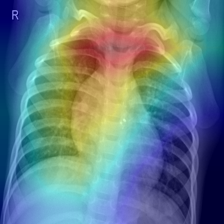
\includegraphics[width=\textwidth]{resnet18_false_negative_pneumonia_person154_bacteria_7.png}
\caption{resnet18 false negative pneumonia person154 bacteria 7}
\end{subfigure}\hfill
\begin{subfigure}{0.40\textwidth}
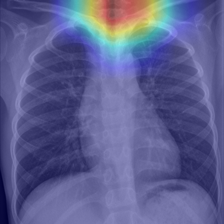
\includegraphics[width=\textwidth]{resnet18_false_positive_normal_IM-0006-0001.png}
\caption{resnet18 false positive normal IM-0006-0001}
\end{subfigure}\\[0.6em]
\begin{subfigure}{0.40\textwidth}
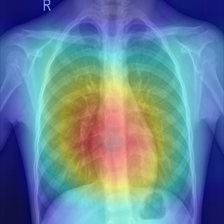
\includegraphics[width=\textwidth]{resnet18_true_negative_normal_IM-0001-0001.png}
\caption{resnet18 true negative normal IM-0001-0001}
\end{subfigure}\hfill
\begin{subfigure}{0.40\textwidth}
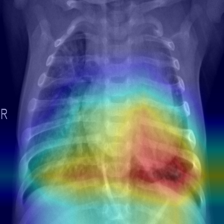
\includegraphics[width=\textwidth]{resnet18_true_positive_pneumonia_person100_bacteria_4.png}
\caption{resnet18 true positive pneumonia person100 bacteria 4}
\end{subfigure}
\caption{Binary Grad-CAM overlays for ResNet18 (TP / TN / FP / FN).}
\label{fig:app_gcb}
\end{figure}
\FloatBarrier

\begin{figure}[h]
\centering
\begin{subfigure}{0.31\textwidth}
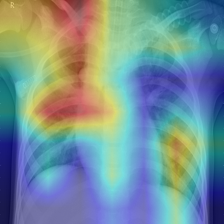
\includegraphics[width=\textwidth]{densenet121_3class_wrong_VIRUS_as_BACTERIA_person10_virus_35.png}
\caption{densenet121 3class wrong VIRUS as BACTERIA person10 virus 35}
\end{subfigure}\hfill
\begin{subfigure}{0.31\textwidth}
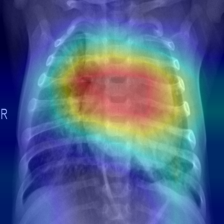
\includegraphics[width=\textwidth]{resnet18_3class_correct_BACTERIA_person100_bacteria_4.png}
\caption{resnet18 3class correct BACTERIA person100 bacteria 4}
\end{subfigure}\hfill
\begin{subfigure}{0.31\textwidth}
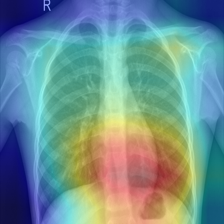
\includegraphics[width=\textwidth]{resnet18_3class_correct_NORMAL_IM-0001-0001.png}
\caption{resnet18 3class correct NORMAL IM-0001-0001}
\end{subfigure}\\[0.6em]
\begin{subfigure}{0.31\textwidth}
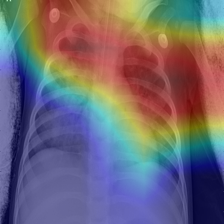
\includegraphics[width=\textwidth]{resnet18_3class_wrong_BACTERIA_as_VIRUS_person110_bacteria_5.png}
\caption{resnet18 3class wrong BACTERIA as VIRUS person110 bacteria 5}
\end{subfigure}\hfill
\begin{subfigure}{0.31\textwidth}
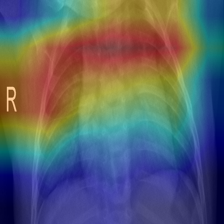
\includegraphics[width=\textwidth]{resnet18_3class_wrong_NORMAL_as_BACTERIA_IM-0022-0001.png}
\caption{resnet18 3class wrong NORMAL as BACTERIA IM-0022-0001}
\end{subfigure}\hfill
\begin{subfigure}{0.31\textwidth}
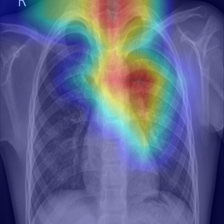
\includegraphics[width=\textwidth]{resnet18_3class_wrong_NORMAL_as_VIRUS_IM-0015-0001.png}
\caption{resnet18 3class wrong NORMAL as VIRUS IM-0015-0001}
\end{subfigure}\\[0.6em]
\begin{subfigure}{0.31\textwidth}
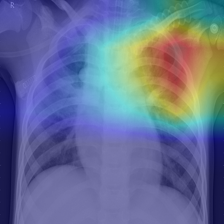
\includegraphics[width=\textwidth]{resnet18_3class_wrong_VIRUS_as_BACTERIA_person10_virus_35.png}
\caption{resnet18 3class wrong VIRUS as BACTERIA person10 virus 35}
\end{subfigure}
\caption{Additional three-class Grad-CAM overlays (ResNet18, plus the DenseNet121 VIRUS-as-BACTERIA case).}
\label{fig:app_gc3b}
\end{figure}
\FloatBarrier

\begin{figure}[h]
\centering
\begin{subfigure}{0.75\textwidth}
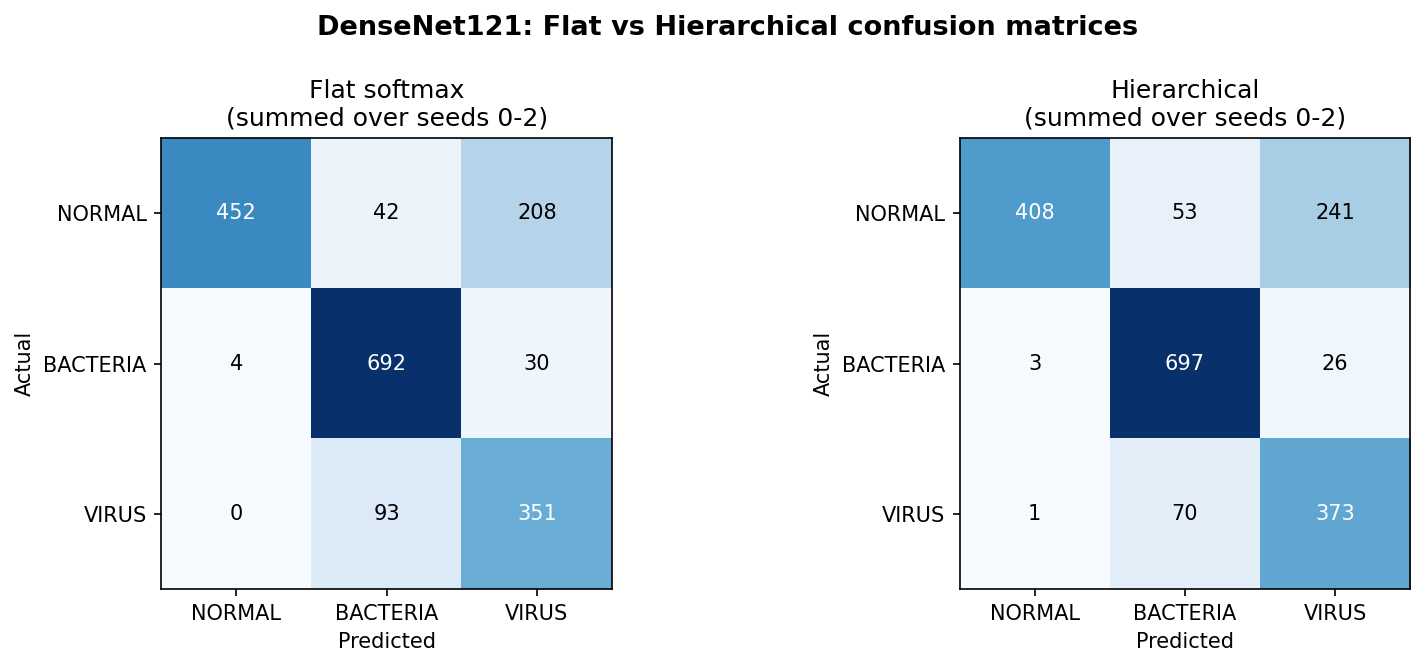
\includegraphics[width=\textwidth]{densenet121_flat_vs_hierarchical_confusion.png}
\caption{densenet121 flat vs hierarchical confusion}
\end{subfigure}\\[0.8em]
\begin{subfigure}{0.75\textwidth}
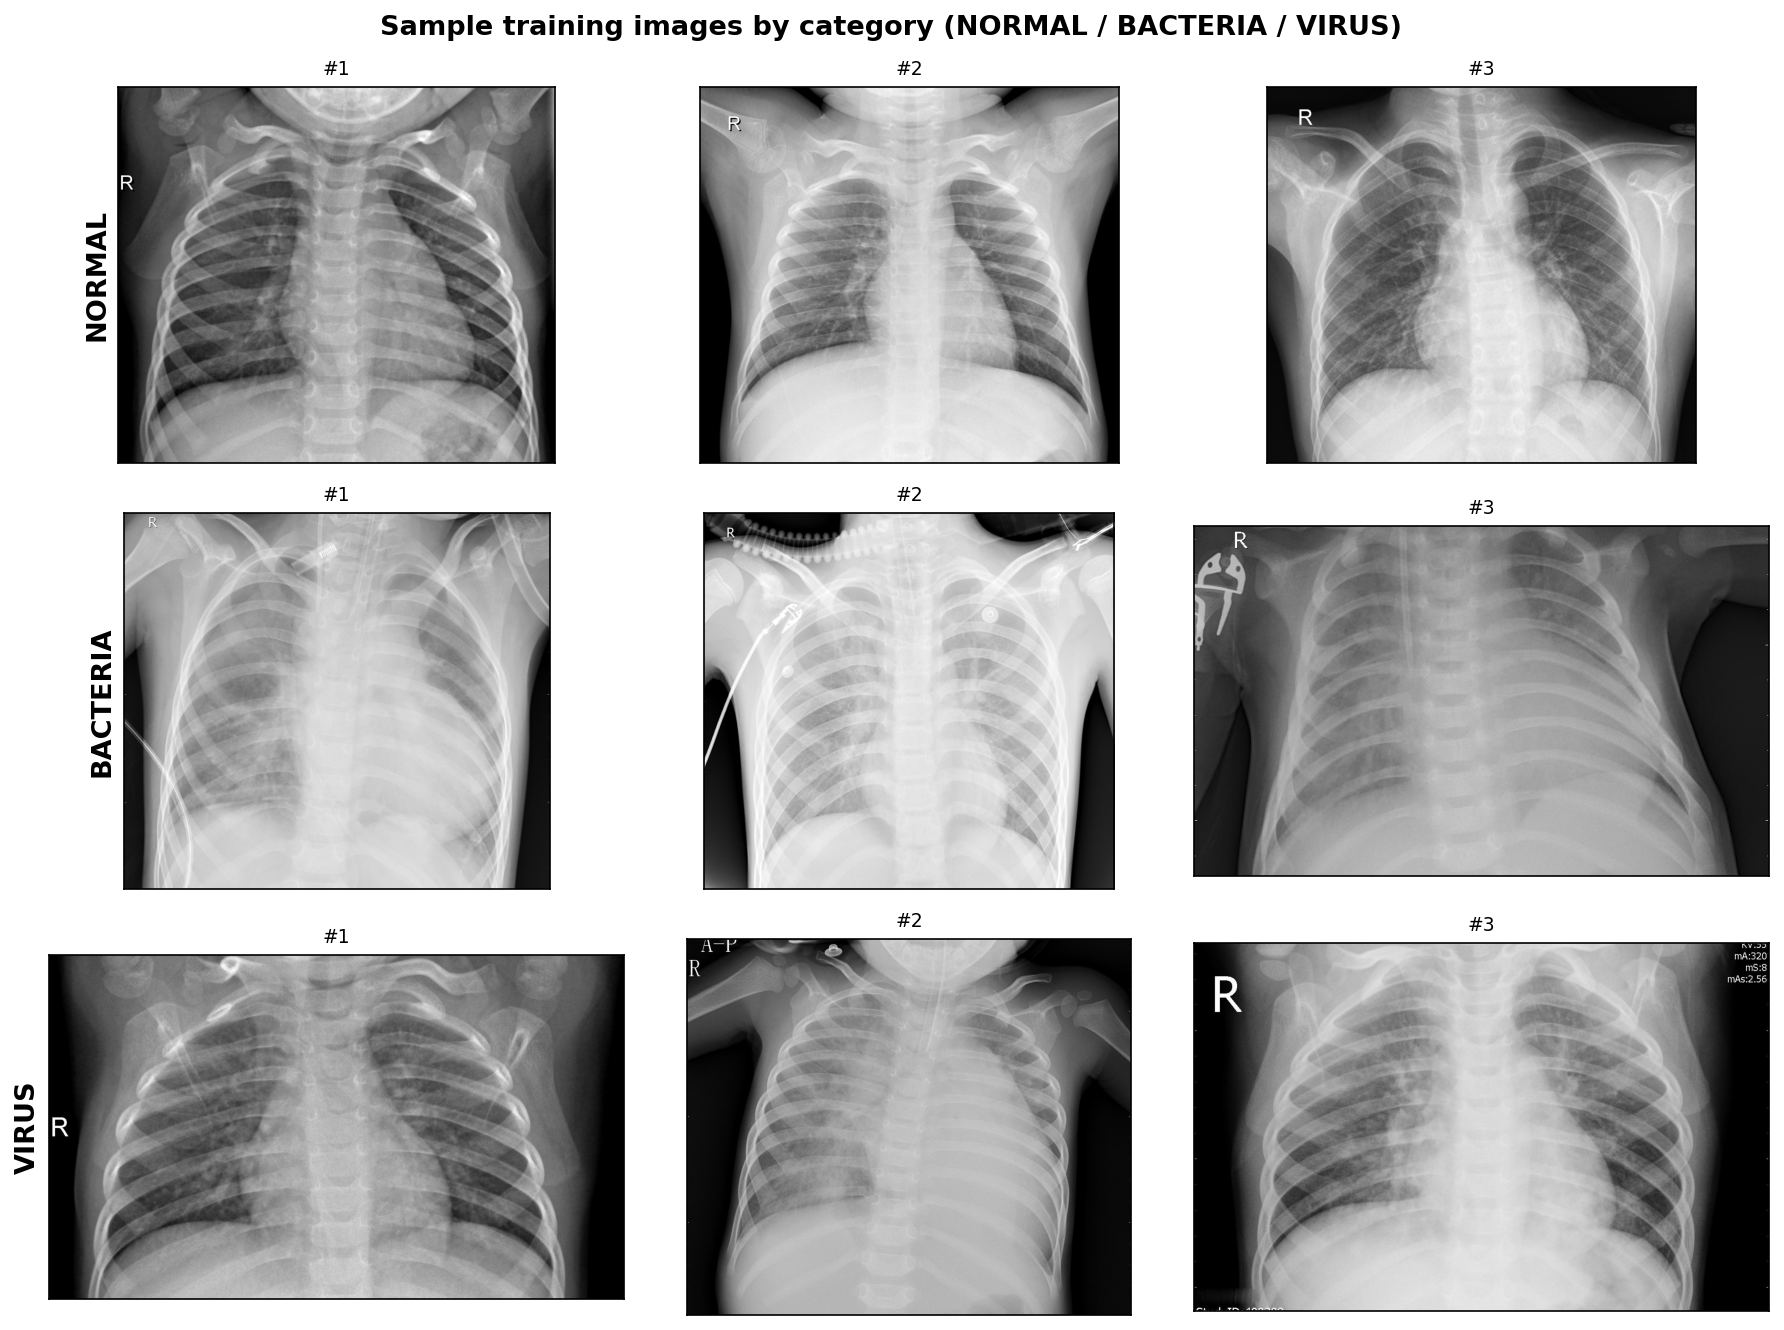
\includegraphics[width=\textwidth]{sample_images_three_class.png}
\caption{sample images three class}
\end{subfigure}
\caption{Dataset sample images per class, and the flat-vs-hierarchical confusion matrices.}
\label{fig:app_other2}
\end{figure}
\FloatBarrier


\end{document}
